\documentclass[twoside]{book}

% Packages required by doxygen
\usepackage{fixltx2e}
\usepackage{calc}
\usepackage{doxygen}
\usepackage[export]{adjustbox} % also loads graphicx
\usepackage{graphicx}
\usepackage[utf8]{inputenc}
\usepackage{makeidx}
\usepackage{multicol}
\usepackage{multirow}
\PassOptionsToPackage{warn}{textcomp}
\usepackage{textcomp}
\usepackage[nointegrals]{wasysym}
\usepackage[table]{xcolor}

% NLS support packages
\usepackage[french]{babel}

% Font selection
\usepackage[T1]{fontenc}
\usepackage[scaled=.90]{helvet}
\usepackage{courier}
\usepackage{amssymb}
\usepackage{sectsty}
\renewcommand{\familydefault}{\sfdefault}
\allsectionsfont{%
  \fontseries{bc}\selectfont%
  \color{darkgray}%
}
\renewcommand{\DoxyLabelFont}{%
  \fontseries{bc}\selectfont%
  \color{darkgray}%
}
\newcommand{\+}{\discretionary{\mbox{\scriptsize$\hookleftarrow$}}{}{}}

% Page & text layout
\usepackage{geometry}
\geometry{%
  a4paper,%
  top=2.5cm,%
  bottom=2.5cm,%
  left=2.5cm,%
  right=2.5cm%
}
\tolerance=750
\hfuzz=15pt
\hbadness=750
\setlength{\emergencystretch}{15pt}
\setlength{\parindent}{0cm}
\setlength{\parskip}{3ex plus 2ex minus 2ex}
\makeatletter
\renewcommand{\paragraph}{%
  \@startsection{paragraph}{4}{0ex}{-1.0ex}{1.0ex}{%
    \normalfont\normalsize\bfseries\SS@parafont%
  }%
}
\renewcommand{\subparagraph}{%
  \@startsection{subparagraph}{5}{0ex}{-1.0ex}{1.0ex}{%
    \normalfont\normalsize\bfseries\SS@subparafont%
  }%
}
\makeatother

% Headers & footers
\usepackage{fancyhdr}
\pagestyle{fancyplain}
\fancyhead[LE]{\fancyplain{}{\bfseries\thepage}}
\fancyhead[CE]{\fancyplain{}{}}
\fancyhead[RE]{\fancyplain{}{\bfseries\leftmark}}
\fancyhead[LO]{\fancyplain{}{\bfseries\rightmark}}
\fancyhead[CO]{\fancyplain{}{}}
\fancyhead[RO]{\fancyplain{}{\bfseries\thepage}}
\fancyfoot[LE]{\fancyplain{}{}}
\fancyfoot[CE]{\fancyplain{}{}}
\fancyfoot[RE]{\fancyplain{}{\bfseries\scriptsize Généré par Doxygen }}
\fancyfoot[LO]{\fancyplain{}{\bfseries\scriptsize Généré par Doxygen }}
\fancyfoot[CO]{\fancyplain{}{}}
\fancyfoot[RO]{\fancyplain{}{}}
\renewcommand{\footrulewidth}{0.4pt}
\renewcommand{\chaptermark}[1]{%
  \markboth{#1}{}%
}
\renewcommand{\sectionmark}[1]{%
  \markright{\thesection\ #1}%
}

% Indices & bibliography
\usepackage{natbib}
\usepackage[titles]{tocloft}
\setcounter{tocdepth}{3}
\setcounter{secnumdepth}{5}
\makeindex

% Hyperlinks (required, but should be loaded last)
\usepackage{ifpdf}
\ifpdf
  \usepackage[pdftex,pagebackref=true]{hyperref}
\else
  \usepackage[ps2pdf,pagebackref=true]{hyperref}
\fi
\hypersetup{%
  colorlinks=true,%
  linkcolor=blue,%
  citecolor=blue,%
  unicode%
}

% Custom commands
\newcommand{\clearemptydoublepage}{%
  \newpage{\pagestyle{empty}\cleardoublepage}%
}

\usepackage{caption}
\captionsetup{labelsep=space,justification=centering,font={bf},singlelinecheck=off,skip=4pt,position=top}

%===== C O N T E N T S =====

\begin{document}

% Titlepage & ToC
\hypersetup{pageanchor=false,
             bookmarksnumbered=true,
             pdfencoding=unicode
            }
\pagenumbering{alph}
\begin{titlepage}
\vspace*{7cm}
\begin{center}%
{\Large Projet Recette I\+HM \\[1ex]\large 1.\+5 }\\
\vspace*{1cm}
{\large Généré par Doxygen 1.8.13}\\
\end{center}
\end{titlepage}
\clearemptydoublepage
\pagenumbering{roman}
\tableofcontents
\clearemptydoublepage
\pagenumbering{arabic}
\hypersetup{pageanchor=true}

%--- Begin generated contents ---
\chapter{My Personal Index Page}
\label{index}\hypertarget{index}{}\hypertarget{index_intro_sec}{}\section{Introduction}\label{index_intro_sec}
This is the introduction.\hypertarget{index_install_sec}{}\section{Installation}\label{index_install_sec}
\hypertarget{index_step1}{}\subsection{Step 1\+: Opening the box}\label{index_step1}
etc... 
\chapter{Projet Recette json}
\label{autotoc_md0}
\Hypertarget{autotoc_md0}
\subparagraph*{Projet de parsing de recette au format json.}

\href{https://nodesource.com/products/nsolid}{\tt }

\href{https://etulab.univ-amu.fr/f19003179/projet-recette-json}{\tt }\hypertarget{autotoc_md0_autotoc_md1}{}\section{Présentation du projet}\label{autotoc_md0_autotoc_md1}
Cette application s\textquotesingle{}inscrit dans le cadre du projet d\textquotesingle{}Interface Homme-\/\+Machine. Ce projet à été commandité par Mr. Raffin dans le cadre du module \href{https://fr.wikipedia.org/wiki/Interactions_homme-machine}{\tt I\+HM}. Ce projet à été réalisé par deux étudiants en D\+UT Informatique sur le site \href{https://fr.wikipedia.org/wiki/Arles}{\tt d\textquotesingle{}Arles}.\hypertarget{autotoc_md0_autotoc_md2}{}\subsection{Fonctionnalités}\label{autotoc_md0_autotoc_md2}

\begin{DoxyItemize}
\item Importer un fichier au format \href{https://fr.wikipedia.org/wiki/Portable_Document_Format}{\tt json}
\item Changer l\textquotesingle{}étape de la recette en appuyant sur les boutons suivant/précédent
\item Calcul interne du temps nécessaire à la préparation de la recette
\item Affichage des ingrédients nécessaires à la préparation de la recette
\item Informations et rapport avec la recette et bien d\textquotesingle{}autres encore...
\end{DoxyItemize}\hypertarget{autotoc_md0_autotoc_md3}{}\subsection{Fonctionnement et Classes}\label{autotoc_md0_autotoc_md3}
Pour plus de précision sur le fonctionnement interne de l\textquotesingle{}application et les interractions entre les classes veuillez consulter la documentation \href{https://fr.wikipedia.org/wiki/Portable_Document_Format}{\tt pdf}.

Développé en mai 2020 par Lucas Pollet et Arsène Fougerouse 
\chapter{Index des espaces de nommage}
\doxysection{Namespace List}
Here is a list of all namespaces with brief descriptions\+:\begin{DoxyCompactList}
\item\contentsline{section}{\mbox{\hyperlink{namespaceUi}{Ui}} }{\pageref{namespaceUi}}{}
\end{DoxyCompactList}

\chapter{Index hiérarchique}
\section{Class Hierarchy}
This inheritance list is sorted roughly, but not completely, alphabetically\+:\begin{DoxyCompactList}
\item \contentsline{section}{lecture\+\_\+json}{\pageref{classlecture__json}}{}
\item Q\+Main\+Window\begin{DoxyCompactList}
\item \contentsline{section}{Main\+Window}{\pageref{classMainWindow}}{}
\item \contentsline{section}{Main\+Window\+Launch\+Dialog}{\pageref{classMainWindowLaunchDialog}}{}
\end{DoxyCompactList}
\item Q\+Object\begin{DoxyCompactList}
\item \contentsline{section}{Recette}{\pageref{classRecette}}{}
\end{DoxyCompactList}
\item \contentsline{section}{traitement}{\pageref{classtraitement}}{}
\end{DoxyCompactList}

\chapter{Index des classes}
\section{Class List}
Here are the classes, structs, unions and interfaces with brief descriptions\+:\begin{DoxyCompactList}
\item\contentsline{section}{\hyperlink{classlecture__json}{lecture\+\_\+json} }{\pageref{classlecture__json}}{}
\item\contentsline{section}{\hyperlink{classMainWindow}{Main\+Window} }{\pageref{classMainWindow}}{}
\item\contentsline{section}{\hyperlink{classMainWindowLaunchDialog}{Main\+Window\+Launch\+Dialog} }{\pageref{classMainWindowLaunchDialog}}{}
\item\contentsline{section}{\hyperlink{classRecette}{Recette} }{\pageref{classRecette}}{}
\item\contentsline{section}{\hyperlink{classtraitement}{traitement} }{\pageref{classtraitement}}{}
\end{DoxyCompactList}

\chapter{Index des fichiers}
\doxysection{File List}
Here is a list of all documented files with brief descriptions\+:\begin{DoxyCompactList}
\item\contentsline{section}{\mbox{\hyperlink{lecture__json_8cpp}{lecture\+\_\+json.\+cpp}} \\*Classe gérant la lecture du fichier json }{\pageref{lecture__json_8cpp}}{}
\item\contentsline{section}{\mbox{\hyperlink{lecture__json_8h}{lecture\+\_\+json.\+h}} \\*Classe gérant la lecture du fichier json }{\pageref{lecture__json_8h}}{}
\item\contentsline{section}{\mbox{\hyperlink{main_8cpp}{main.\+cpp}} \\*Classe principale qui permet de lancer la première fenetre }{\pageref{main_8cpp}}{}
\item\contentsline{section}{\mbox{\hyperlink{mainwindow_8cpp}{mainwindow.\+cpp}} \\*Classe de la fenêtre permettant l\textquotesingle{}affichage de la recette }{\pageref{mainwindow_8cpp}}{}
\item\contentsline{section}{\mbox{\hyperlink{mainwindow_8h}{mainwindow.\+h}} \\*Classe de la fenêtre permettant l\textquotesingle{}affichage de la recette }{\pageref{mainwindow_8h}}{}
\item\contentsline{section}{\mbox{\hyperlink{mainwindowlaunchdialog_8cpp}{mainwindowlaunchdialog.\+cpp}} \\*Classe de la fenêtre permettant le choix du fichier json de recette }{\pageref{mainwindowlaunchdialog_8cpp}}{}
\item\contentsline{section}{\mbox{\hyperlink{mainwindowlaunchdialog_8h}{mainwindowlaunchdialog.\+h}} \\*Classe de la fenêtre permettant le choix du fichier json de recette }{\pageref{mainwindowlaunchdialog_8h}}{}
\item\contentsline{section}{\mbox{\hyperlink{recette_8cpp}{recette.\+cpp}} \\*Classe permettant la gestion et le stockage de la recette }{\pageref{recette_8cpp}}{}
\item\contentsline{section}{\mbox{\hyperlink{recette_8h}{recette.\+h}} \\*Classe permettant la gestion et le stockage de la recette }{\pageref{recette_8h}}{}
\item\contentsline{section}{\mbox{\hyperlink{traitement_8cpp}{traitement.\+cpp}} \\*Classe permettant le traitement json }{\pageref{traitement_8cpp}}{}
\item\contentsline{section}{\mbox{\hyperlink{traitement_8h}{traitement.\+h}} \\*Classe permettant le traitement json }{\pageref{traitement_8h}}{}
\end{DoxyCompactList}

\chapter{Documentation des espaces de nommage}
\hypertarget{namespaceUi}{}\section{Ui Namespace Reference}
\label{namespaceUi}\index{Ui@{Ui}}

\chapter{Documentation des classes}
\hypertarget{classlecture__json}{}\section{Référence de la classe lecture\+\_\+json}
\label{classlecture__json}\index{lecture\+\_\+json@{lecture\+\_\+json}}


{\ttfamily \#include $<$lecture\+\_\+json.\+h$>$}



Graphe d\textquotesingle{}héritage de lecture\+\_\+json\+:\nopagebreak
\begin{figure}[H]
\begin{center}
\leavevmode
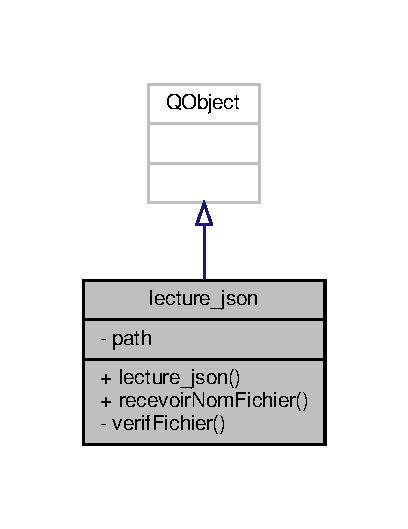
\includegraphics[width=196pt]{classlecture__json__inherit__graph}
\end{center}
\end{figure}


Graphe de collaboration de lecture\+\_\+json\+:\nopagebreak
\begin{figure}[H]
\begin{center}
\leavevmode
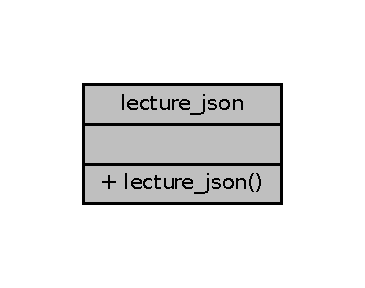
\includegraphics[width=196pt]{classlecture__json__coll__graph}
\end{center}
\end{figure}
\subsection*{Connecteurs publics}
\begin{DoxyCompactItemize}
\item 
void \hyperlink{classlecture__json_a539bb092addd4ee4c75834e4ca413ee7}{recevoir\+Nom\+Fichier} (Q\+String \hyperlink{classlecture__json_addfbc41d56e266180e4a120ba3cd1c61}{path})
\begin{DoxyCompactList}\small\item\em slot qui modifie la donnée membre path \end{DoxyCompactList}\end{DoxyCompactItemize}
\subsection*{Signaux}
\begin{DoxyCompactItemize}
\item 
void \hyperlink{classlecture__json_a62f7f4bea2c9579c37bea5b14177a5db}{envoie\+Doc\+Json} (Q\+Json\+Document doc\+Json)
\begin{DoxyCompactList}\small\item\em signal qui envoie le fichier de recette \end{DoxyCompactList}\end{DoxyCompactItemize}
\subsection*{Fonctions membres publiques}
\begin{DoxyCompactItemize}
\item 
\hyperlink{classlecture__json_a4b8226b61ad6f1112038dde13e207b4f}{lecture\+\_\+json} (Q\+Object $\ast$parent=nullptr)
\begin{DoxyCompactList}\small\item\em constructeur de la fonction \hyperlink{classlecture__json}{lecture\+\_\+json} \end{DoxyCompactList}\end{DoxyCompactItemize}
\subsection*{Fonctions membres privées}
\begin{DoxyCompactItemize}
\item 
void \hyperlink{classlecture__json_a88650de275287dc5ddd31f50bdd6d767}{verif\+Fichier} ()
\begin{DoxyCompactList}\small\item\em fonction qui vérifie si le fichier est lisible et interpretable. \end{DoxyCompactList}\end{DoxyCompactItemize}
\subsection*{Attributs privés}
\begin{DoxyCompactItemize}
\item 
Q\+String \hyperlink{classlecture__json_addfbc41d56e266180e4a120ba3cd1c61}{path}
\end{DoxyCompactItemize}


\subsection{Documentation des constructeurs et destructeur}
\mbox{\Hypertarget{classlecture__json_a4b8226b61ad6f1112038dde13e207b4f}\label{classlecture__json_a4b8226b61ad6f1112038dde13e207b4f}} 
\index{lecture\+\_\+json@{lecture\+\_\+json}!lecture\+\_\+json@{lecture\+\_\+json}}
\index{lecture\+\_\+json@{lecture\+\_\+json}!lecture\+\_\+json@{lecture\+\_\+json}}
\subsubsection{\texorpdfstring{lecture\+\_\+json()}{lecture\_json()}}
{\footnotesize\ttfamily lecture\+\_\+json\+::lecture\+\_\+json (\begin{DoxyParamCaption}\item[{Q\+Object $\ast$}]{parent = {\ttfamily nullptr} }\end{DoxyParamCaption})\hspace{0.3cm}{\ttfamily [explicit]}}



constructeur de la fonction \hyperlink{classlecture__json}{lecture\+\_\+json} 


\begin{DoxyParams}{Paramètres}
{\em parent} & \+: précise si le widget hérite d\textquotesingle{}une autre fenêtre \\
\hline
\end{DoxyParams}


\subsection{Documentation des fonctions membres}
\mbox{\Hypertarget{classlecture__json_a62f7f4bea2c9579c37bea5b14177a5db}\label{classlecture__json_a62f7f4bea2c9579c37bea5b14177a5db}} 
\index{lecture\+\_\+json@{lecture\+\_\+json}!envoie\+Doc\+Json@{envoie\+Doc\+Json}}
\index{envoie\+Doc\+Json@{envoie\+Doc\+Json}!lecture\+\_\+json@{lecture\+\_\+json}}
\subsubsection{\texorpdfstring{envoie\+Doc\+Json}{envoieDocJson}}
{\footnotesize\ttfamily void lecture\+\_\+json\+::envoie\+Doc\+Json (\begin{DoxyParamCaption}\item[{Q\+Json\+Document}]{doc\+Json }\end{DoxyParamCaption})\hspace{0.3cm}{\ttfamily [signal]}}



signal qui envoie le fichier de recette 

\begin{DoxySeeAlso}{Voir également}
\hyperlink{classlecture__json_a62f7f4bea2c9579c37bea5b14177a5db}{envoie\+Doc\+Json(\+Q\+Json\+Document)} 
\end{DoxySeeAlso}

\begin{DoxyParams}{Paramètres}
{\em doc\+Json} & \+: le document au format json \\
\hline
\end{DoxyParams}
\mbox{\Hypertarget{classlecture__json_a539bb092addd4ee4c75834e4ca413ee7}\label{classlecture__json_a539bb092addd4ee4c75834e4ca413ee7}} 
\index{lecture\+\_\+json@{lecture\+\_\+json}!recevoir\+Nom\+Fichier@{recevoir\+Nom\+Fichier}}
\index{recevoir\+Nom\+Fichier@{recevoir\+Nom\+Fichier}!lecture\+\_\+json@{lecture\+\_\+json}}
\subsubsection{\texorpdfstring{recevoir\+Nom\+Fichier}{recevoirNomFichier}}
{\footnotesize\ttfamily lecture\+\_\+json\+::recevoir\+Nom\+Fichier (\begin{DoxyParamCaption}\item[{Q\+String}]{path }\end{DoxyParamCaption})\hspace{0.3cm}{\ttfamily [slot]}}



slot qui modifie la donnée membre path 


\begin{DoxyParams}{Paramètres}
{\em path} & \+: Q\+String qui spécifie le chemin du fichier \\
\hline
\end{DoxyParams}
\mbox{\Hypertarget{classlecture__json_a88650de275287dc5ddd31f50bdd6d767}\label{classlecture__json_a88650de275287dc5ddd31f50bdd6d767}} 
\index{lecture\+\_\+json@{lecture\+\_\+json}!verif\+Fichier@{verif\+Fichier}}
\index{verif\+Fichier@{verif\+Fichier}!lecture\+\_\+json@{lecture\+\_\+json}}
\subsubsection{\texorpdfstring{verif\+Fichier()}{verifFichier()}}
{\footnotesize\ttfamily lecture\+\_\+json\+::verif\+Fichier (\begin{DoxyParamCaption}{ }\end{DoxyParamCaption})\hspace{0.3cm}{\ttfamily [private]}}



fonction qui vérifie si le fichier est lisible et interpretable. 



\subsection{Documentation des données membres}
\mbox{\Hypertarget{classlecture__json_addfbc41d56e266180e4a120ba3cd1c61}\label{classlecture__json_addfbc41d56e266180e4a120ba3cd1c61}} 
\index{lecture\+\_\+json@{lecture\+\_\+json}!path@{path}}
\index{path@{path}!lecture\+\_\+json@{lecture\+\_\+json}}
\subsubsection{\texorpdfstring{path}{path}}
{\footnotesize\ttfamily Q\+String lecture\+\_\+json\+::path\hspace{0.3cm}{\ttfamily [private]}}

path\+: chemin d\textquotesingle{}accès du fichier json 

La documentation de cette classe a été générée à partir des fichiers suivants \+:\begin{DoxyCompactItemize}
\item 
\hyperlink{lecture__json_8h}{lecture\+\_\+json.\+h}\item 
\hyperlink{lecture__json_8cpp}{lecture\+\_\+json.\+cpp}\end{DoxyCompactItemize}

\hypertarget{classMainWindow}{}\section{Référence de la classe Main\+Window}
\label{classMainWindow}\index{Main\+Window@{Main\+Window}}


{\ttfamily \#include $<$mainwindow.\+h$>$}



Graphe d\textquotesingle{}héritage de Main\+Window\+:\nopagebreak
\begin{figure}[H]
\begin{center}
\leavevmode
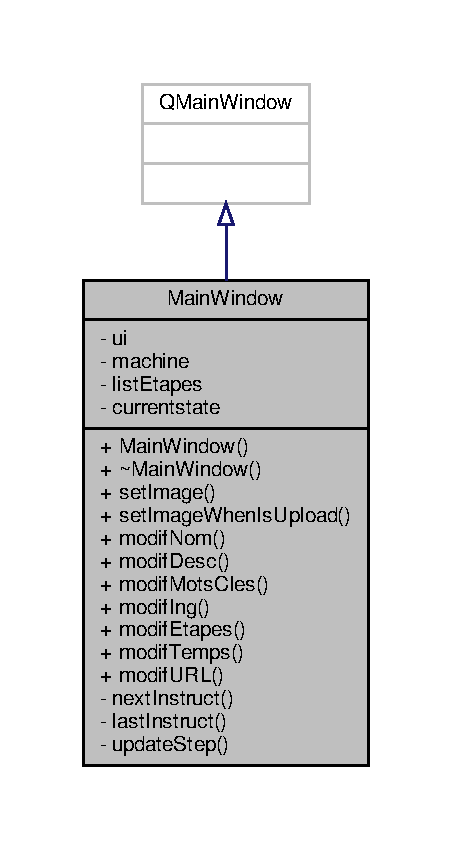
\includegraphics[width=217pt]{classMainWindow__inherit__graph}
\end{center}
\end{figure}


Graphe de collaboration de Main\+Window\+:\nopagebreak
\begin{figure}[H]
\begin{center}
\leavevmode
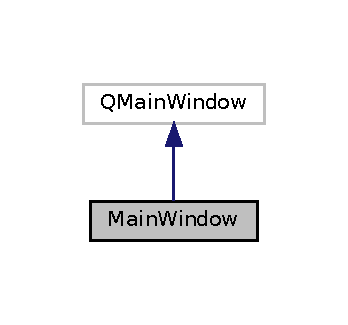
\includegraphics[height=550pt]{classMainWindow__coll__graph}
\end{center}
\end{figure}
\subsection*{Connecteurs publics}
\begin{DoxyCompactItemize}
\item 
void \hyperlink{classMainWindow_aaddccbd976fda27cf2d17b9f43dbc486}{set\+Image} (Q\+String)
\item 
void \hyperlink{classMainWindow_ae58368ff237b1f298381a0aeaf8e7290}{set\+Image\+When\+Is\+Upload} (Q\+Network\+Reply $\ast$)
\item 
void \hyperlink{classMainWindow_ac154b320efe8998a85a93f1c41ace7e4}{modif\+Nom} (Q\+String)
\begin{DoxyCompactList}\small\item\em slot qui modifie le nom de la recette \end{DoxyCompactList}\item 
void \hyperlink{classMainWindow_a77ada7a541d869ea7f3647900ba6f6df}{modif\+Desc} (Q\+String)
\begin{DoxyCompactList}\small\item\em slot qui modifie la description \end{DoxyCompactList}\item 
void \hyperlink{classMainWindow_ae9b5aeb3f3b89a40008486d1329a68bc}{modif\+Mots\+Cles} (Q\+String)
\begin{DoxyCompactList}\small\item\em slot qui modifie les mots cles \end{DoxyCompactList}\item 
void \hyperlink{classMainWindow_a64a5116401b4a54c55c6a7d34fc7ec93}{modif\+Ing} (Q\+String\+List)
\begin{DoxyCompactList}\small\item\em slot qui modifie la liste des ingrédients \end{DoxyCompactList}\item 
void \hyperlink{classMainWindow_a1a85241ab332ebb026638ff0a6df83e0}{modif\+Etapes} (Q\+String\+List)
\begin{DoxyCompactList}\small\item\em slot qui modifie le la liste des etapes \end{DoxyCompactList}\item 
void \hyperlink{classMainWindow_ab49cf9603a1a539ca19623eac88b86c2}{modif\+Temps} (Q\+String)
\begin{DoxyCompactList}\small\item\em slot qui modifie le temps nécessaire pour préparer la recette \end{DoxyCompactList}\item 
void \hyperlink{classMainWindow_a3620273f0e53b380d70df636400e8519}{modif\+U\+RL} (Q\+String)
\begin{DoxyCompactList}\small\item\em slot qui modifie l\textquotesingle{}url pour accéder à la recette \end{DoxyCompactList}\end{DoxyCompactItemize}
\subsection*{Signaux}
\begin{DoxyCompactItemize}
\item 
void \hyperlink{classMainWindow_a2cd7fd54c497cd6a073ad43857266890}{end\+Change\+State} ()
\begin{DoxyCompactList}\small\item\em signal qui annonce la fin du changement d\textquotesingle{}état \end{DoxyCompactList}\end{DoxyCompactItemize}
\subsection*{Fonctions membres publiques}
\begin{DoxyCompactItemize}
\item 
\hyperlink{classMainWindow_a996c5a2b6f77944776856f08ec30858d}{Main\+Window} (Q\+Widget $\ast$parent=nullptr)
\begin{DoxyCompactList}\small\item\em constructeur de la fonction \hyperlink{classMainWindow}{Main\+Window} \end{DoxyCompactList}\item 
\hyperlink{classMainWindow_ae98d00a93bc118200eeef9f9bba1dba7}{$\sim$\+Main\+Window} ()
\begin{DoxyCompactList}\small\item\em destructeur de la fonction \hyperlink{classMainWindow}{Main\+Window} \end{DoxyCompactList}\end{DoxyCompactItemize}
\subsection*{Connecteurs privés}
\begin{DoxyCompactItemize}
\item 
void \hyperlink{classMainWindow_a0b79b7ea071fc3a4baa45f8394052ffd}{next\+Instruct} ()
\begin{DoxyCompactList}\small\item\em fonction qui permet de passer à l\textquotesingle{}instruction suivante \end{DoxyCompactList}\item 
void \hyperlink{classMainWindow_a715f753a6c46e3f10565a5a1b849ee86}{last\+Instruct} ()
\begin{DoxyCompactList}\small\item\em fonction qui permet de passer à l\textquotesingle{}instruction précédente \end{DoxyCompactList}\item 
void \hyperlink{classMainWindow_a344d21527850380c306fe7ac165321bd}{update\+Step} ()
\begin{DoxyCompactList}\small\item\em fonction qui met à jour l\textquotesingle{}instruction affiché à l\textquotesingle{}écran \end{DoxyCompactList}\end{DoxyCompactItemize}
\subsection*{Attributs privés}
\begin{DoxyCompactItemize}
\item 
\hyperlink{classUi_1_1MainWindow}{Ui\+::\+Main\+Window} $\ast$ \hyperlink{classMainWindow_a35466a70ed47252a0191168126a352a5}{ui}
\item 
Q\+State\+Machine $\ast$ \hyperlink{classMainWindow_af5f0afb6c5f81e4438f98f93f918ea8b}{machine}
\item 
Q\+String\+List \hyperlink{classMainWindow_a1290f4c9df65fb27c870753aa2b24a88}{list\+Etapes}
\item 
int \hyperlink{classMainWindow_aa7fb75eed49d7eaa019f64577fa11b05}{currentstate} = 0
\end{DoxyCompactItemize}


\subsection{Documentation des constructeurs et destructeur}
\mbox{\Hypertarget{classMainWindow_a996c5a2b6f77944776856f08ec30858d}\label{classMainWindow_a996c5a2b6f77944776856f08ec30858d}} 
\index{Main\+Window@{Main\+Window}!Main\+Window@{Main\+Window}}
\index{Main\+Window@{Main\+Window}!Main\+Window@{Main\+Window}}
\subsubsection{\texorpdfstring{Main\+Window()}{MainWindow()}}
{\footnotesize\ttfamily Main\+Window\+::\+Main\+Window (\begin{DoxyParamCaption}\item[{Q\+Widget $\ast$}]{parent = {\ttfamily nullptr} }\end{DoxyParamCaption})}



constructeur de la fonction \hyperlink{classMainWindow}{Main\+Window} 


\begin{DoxyParams}{Paramètres}
{\em parent} & \+: précise si le widget hérite d\textquotesingle{}une autre fenêtre \\
\hline
\end{DoxyParams}
\mbox{\Hypertarget{classMainWindow_ae98d00a93bc118200eeef9f9bba1dba7}\label{classMainWindow_ae98d00a93bc118200eeef9f9bba1dba7}} 
\index{Main\+Window@{Main\+Window}!````~Main\+Window@{$\sim$\+Main\+Window}}
\index{````~Main\+Window@{$\sim$\+Main\+Window}!Main\+Window@{Main\+Window}}
\subsubsection{\texorpdfstring{$\sim$\+Main\+Window()}{~MainWindow()}}
{\footnotesize\ttfamily Main\+Window\+::$\sim$\+Main\+Window (\begin{DoxyParamCaption}{ }\end{DoxyParamCaption})}



destructeur de la fonction \hyperlink{classMainWindow}{Main\+Window} 



\subsection{Documentation des fonctions membres}
\mbox{\Hypertarget{classMainWindow_a2cd7fd54c497cd6a073ad43857266890}\label{classMainWindow_a2cd7fd54c497cd6a073ad43857266890}} 
\index{Main\+Window@{Main\+Window}!end\+Change\+State@{end\+Change\+State}}
\index{end\+Change\+State@{end\+Change\+State}!Main\+Window@{Main\+Window}}
\subsubsection{\texorpdfstring{end\+Change\+State}{endChangeState}}
{\footnotesize\ttfamily void Main\+Window\+::end\+Change\+State (\begin{DoxyParamCaption}{ }\end{DoxyParamCaption})\hspace{0.3cm}{\ttfamily [signal]}}



signal qui annonce la fin du changement d\textquotesingle{}état 

\begin{DoxySeeAlso}{Voir également}
\hyperlink{classMainWindow_a2cd7fd54c497cd6a073ad43857266890}{end\+Change\+State()} 
\end{DoxySeeAlso}
\mbox{\Hypertarget{classMainWindow_a715f753a6c46e3f10565a5a1b849ee86}\label{classMainWindow_a715f753a6c46e3f10565a5a1b849ee86}} 
\index{Main\+Window@{Main\+Window}!last\+Instruct@{last\+Instruct}}
\index{last\+Instruct@{last\+Instruct}!Main\+Window@{Main\+Window}}
\subsubsection{\texorpdfstring{last\+Instruct}{lastInstruct}}
{\footnotesize\ttfamily Main\+Window\+::last\+Instruct (\begin{DoxyParamCaption}{ }\end{DoxyParamCaption})\hspace{0.3cm}{\ttfamily [private]}, {\ttfamily [slot]}}



fonction qui permet de passer à l\textquotesingle{}instruction précédente 

\mbox{\Hypertarget{classMainWindow_a77ada7a541d869ea7f3647900ba6f6df}\label{classMainWindow_a77ada7a541d869ea7f3647900ba6f6df}} 
\index{Main\+Window@{Main\+Window}!modif\+Desc@{modif\+Desc}}
\index{modif\+Desc@{modif\+Desc}!Main\+Window@{Main\+Window}}
\subsubsection{\texorpdfstring{modif\+Desc}{modifDesc}}
{\footnotesize\ttfamily Main\+Window\+::modif\+Desc (\begin{DoxyParamCaption}\item[{Q\+String}]{str }\end{DoxyParamCaption})\hspace{0.3cm}{\ttfamily [slot]}}



slot qui modifie la description 


\begin{DoxyParams}{Paramètres}
{\em la} & description sous forme de chaine de caractère \\
\hline
\end{DoxyParams}
\mbox{\Hypertarget{classMainWindow_a1a85241ab332ebb026638ff0a6df83e0}\label{classMainWindow_a1a85241ab332ebb026638ff0a6df83e0}} 
\index{Main\+Window@{Main\+Window}!modif\+Etapes@{modif\+Etapes}}
\index{modif\+Etapes@{modif\+Etapes}!Main\+Window@{Main\+Window}}
\subsubsection{\texorpdfstring{modif\+Etapes}{modifEtapes}}
{\footnotesize\ttfamily Main\+Window\+::modif\+Etapes (\begin{DoxyParamCaption}\item[{Q\+String\+List}]{list }\end{DoxyParamCaption})\hspace{0.3cm}{\ttfamily [slot]}}



slot qui modifie le la liste des etapes 


\begin{DoxyParams}{Paramètres}
{\em les} & étapes sous formes de liste de chaine de caractere \\
\hline
\end{DoxyParams}
\mbox{\Hypertarget{classMainWindow_a64a5116401b4a54c55c6a7d34fc7ec93}\label{classMainWindow_a64a5116401b4a54c55c6a7d34fc7ec93}} 
\index{Main\+Window@{Main\+Window}!modif\+Ing@{modif\+Ing}}
\index{modif\+Ing@{modif\+Ing}!Main\+Window@{Main\+Window}}
\subsubsection{\texorpdfstring{modif\+Ing}{modifIng}}
{\footnotesize\ttfamily Main\+Window\+::modif\+Ing (\begin{DoxyParamCaption}\item[{Q\+String\+List}]{l }\end{DoxyParamCaption})\hspace{0.3cm}{\ttfamily [slot]}}



slot qui modifie la liste des ingrédients 


\begin{DoxyParams}{Paramètres}
{\em les} & ingrédients sous forme de liste de chaine de caractere \\
\hline
\end{DoxyParams}
\mbox{\Hypertarget{classMainWindow_ae9b5aeb3f3b89a40008486d1329a68bc}\label{classMainWindow_ae9b5aeb3f3b89a40008486d1329a68bc}} 
\index{Main\+Window@{Main\+Window}!modif\+Mots\+Cles@{modif\+Mots\+Cles}}
\index{modif\+Mots\+Cles@{modif\+Mots\+Cles}!Main\+Window@{Main\+Window}}
\subsubsection{\texorpdfstring{modif\+Mots\+Cles}{modifMotsCles}}
{\footnotesize\ttfamily Main\+Window\+::modif\+Mots\+Cles (\begin{DoxyParamCaption}\item[{Q\+String}]{str }\end{DoxyParamCaption})\hspace{0.3cm}{\ttfamily [slot]}}



slot qui modifie les mots cles 


\begin{DoxyParams}{Paramètres}
{\em les} & mots cles sous forme de chaine de caractère \\
\hline
\end{DoxyParams}
\mbox{\Hypertarget{classMainWindow_ac154b320efe8998a85a93f1c41ace7e4}\label{classMainWindow_ac154b320efe8998a85a93f1c41ace7e4}} 
\index{Main\+Window@{Main\+Window}!modif\+Nom@{modif\+Nom}}
\index{modif\+Nom@{modif\+Nom}!Main\+Window@{Main\+Window}}
\subsubsection{\texorpdfstring{modif\+Nom}{modifNom}}
{\footnotesize\ttfamily Main\+Window\+::modif\+Nom (\begin{DoxyParamCaption}\item[{Q\+String}]{str }\end{DoxyParamCaption})\hspace{0.3cm}{\ttfamily [slot]}}



slot qui modifie le nom de la recette 


\begin{DoxyParams}{Paramètres}
{\em le} & nom sous forme de chaine de caractère \\
\hline
\end{DoxyParams}
\mbox{\Hypertarget{classMainWindow_ab49cf9603a1a539ca19623eac88b86c2}\label{classMainWindow_ab49cf9603a1a539ca19623eac88b86c2}} 
\index{Main\+Window@{Main\+Window}!modif\+Temps@{modif\+Temps}}
\index{modif\+Temps@{modif\+Temps}!Main\+Window@{Main\+Window}}
\subsubsection{\texorpdfstring{modif\+Temps}{modifTemps}}
{\footnotesize\ttfamily Main\+Window\+::modif\+Temps (\begin{DoxyParamCaption}\item[{Q\+String}]{temps }\end{DoxyParamCaption})\hspace{0.3cm}{\ttfamily [slot]}}



slot qui modifie le temps nécessaire pour préparer la recette 


\begin{DoxyParams}{Paramètres}
{\em les} & différents temps sous forme de liste de chaine de caractère \\
\hline
\end{DoxyParams}
\mbox{\Hypertarget{classMainWindow_a3620273f0e53b380d70df636400e8519}\label{classMainWindow_a3620273f0e53b380d70df636400e8519}} 
\index{Main\+Window@{Main\+Window}!modif\+U\+RL@{modif\+U\+RL}}
\index{modif\+U\+RL@{modif\+U\+RL}!Main\+Window@{Main\+Window}}
\subsubsection{\texorpdfstring{modif\+U\+RL}{modifURL}}
{\footnotesize\ttfamily Main\+Window\+::modif\+U\+RL (\begin{DoxyParamCaption}\item[{Q\+String}]{url }\end{DoxyParamCaption})\hspace{0.3cm}{\ttfamily [slot]}}



slot qui modifie l\textquotesingle{}url pour accéder à la recette 


\begin{DoxyParams}{Paramètres}
{\em l\textquotesingle{}url} & sous forme de chaine de caractère \\
\hline
\end{DoxyParams}
\mbox{\Hypertarget{classMainWindow_a0b79b7ea071fc3a4baa45f8394052ffd}\label{classMainWindow_a0b79b7ea071fc3a4baa45f8394052ffd}} 
\index{Main\+Window@{Main\+Window}!next\+Instruct@{next\+Instruct}}
\index{next\+Instruct@{next\+Instruct}!Main\+Window@{Main\+Window}}
\subsubsection{\texorpdfstring{next\+Instruct}{nextInstruct}}
{\footnotesize\ttfamily Main\+Window\+::next\+Instruct (\begin{DoxyParamCaption}{ }\end{DoxyParamCaption})\hspace{0.3cm}{\ttfamily [private]}, {\ttfamily [slot]}}



fonction qui permet de passer à l\textquotesingle{}instruction suivante 

\mbox{\Hypertarget{classMainWindow_aaddccbd976fda27cf2d17b9f43dbc486}\label{classMainWindow_aaddccbd976fda27cf2d17b9f43dbc486}} 
\index{Main\+Window@{Main\+Window}!set\+Image@{set\+Image}}
\index{set\+Image@{set\+Image}!Main\+Window@{Main\+Window}}
\subsubsection{\texorpdfstring{set\+Image}{setImage}}
{\footnotesize\ttfamily void Main\+Window\+::set\+Image (\begin{DoxyParamCaption}\item[{Q\+String}]{url }\end{DoxyParamCaption})\hspace{0.3cm}{\ttfamily [slot]}}

\mbox{\Hypertarget{classMainWindow_ae58368ff237b1f298381a0aeaf8e7290}\label{classMainWindow_ae58368ff237b1f298381a0aeaf8e7290}} 
\index{Main\+Window@{Main\+Window}!set\+Image\+When\+Is\+Upload@{set\+Image\+When\+Is\+Upload}}
\index{set\+Image\+When\+Is\+Upload@{set\+Image\+When\+Is\+Upload}!Main\+Window@{Main\+Window}}
\subsubsection{\texorpdfstring{set\+Image\+When\+Is\+Upload}{setImageWhenIsUpload}}
{\footnotesize\ttfamily void Main\+Window\+::set\+Image\+When\+Is\+Upload (\begin{DoxyParamCaption}\item[{Q\+Network\+Reply $\ast$}]{reply }\end{DoxyParamCaption})\hspace{0.3cm}{\ttfamily [slot]}}

\mbox{\Hypertarget{classMainWindow_a344d21527850380c306fe7ac165321bd}\label{classMainWindow_a344d21527850380c306fe7ac165321bd}} 
\index{Main\+Window@{Main\+Window}!update\+Step@{update\+Step}}
\index{update\+Step@{update\+Step}!Main\+Window@{Main\+Window}}
\subsubsection{\texorpdfstring{update\+Step}{updateStep}}
{\footnotesize\ttfamily Main\+Window\+::update\+Step (\begin{DoxyParamCaption}{ }\end{DoxyParamCaption})\hspace{0.3cm}{\ttfamily [private]}, {\ttfamily [slot]}}



fonction qui met à jour l\textquotesingle{}instruction affiché à l\textquotesingle{}écran 



\subsection{Documentation des données membres}
\mbox{\Hypertarget{classMainWindow_aa7fb75eed49d7eaa019f64577fa11b05}\label{classMainWindow_aa7fb75eed49d7eaa019f64577fa11b05}} 
\index{Main\+Window@{Main\+Window}!currentstate@{currentstate}}
\index{currentstate@{currentstate}!Main\+Window@{Main\+Window}}
\subsubsection{\texorpdfstring{currentstate}{currentstate}}
{\footnotesize\ttfamily int Main\+Window\+::currentstate = 0\hspace{0.3cm}{\ttfamily [private]}}

int currentstate\+: variable du numero de l\textquotesingle{}instruction actuelle \mbox{\Hypertarget{classMainWindow_a1290f4c9df65fb27c870753aa2b24a88}\label{classMainWindow_a1290f4c9df65fb27c870753aa2b24a88}} 
\index{Main\+Window@{Main\+Window}!list\+Etapes@{list\+Etapes}}
\index{list\+Etapes@{list\+Etapes}!Main\+Window@{Main\+Window}}
\subsubsection{\texorpdfstring{list\+Etapes}{listEtapes}}
{\footnotesize\ttfamily Q\+String\+List Main\+Window\+::list\+Etapes\hspace{0.3cm}{\ttfamily [private]}}

list\+Etapes\+: liste de string contenant la liste des étapes \mbox{\Hypertarget{classMainWindow_af5f0afb6c5f81e4438f98f93f918ea8b}\label{classMainWindow_af5f0afb6c5f81e4438f98f93f918ea8b}} 
\index{Main\+Window@{Main\+Window}!machine@{machine}}
\index{machine@{machine}!Main\+Window@{Main\+Window}}
\subsubsection{\texorpdfstring{machine}{machine}}
{\footnotesize\ttfamily Q\+State\+Machine$\ast$ Main\+Window\+::machine\hspace{0.3cm}{\ttfamily [private]}}

machine\+: machine à état quand on appuie sur les boutons \mbox{\Hypertarget{classMainWindow_a35466a70ed47252a0191168126a352a5}\label{classMainWindow_a35466a70ed47252a0191168126a352a5}} 
\index{Main\+Window@{Main\+Window}!ui@{ui}}
\index{ui@{ui}!Main\+Window@{Main\+Window}}
\subsubsection{\texorpdfstring{ui}{ui}}
{\footnotesize\ttfamily \hyperlink{classUi_1_1MainWindow}{Ui\+::\+Main\+Window}$\ast$ Main\+Window\+::ui\hspace{0.3cm}{\ttfamily [private]}}

ui\+: \hyperlink{classMainWindow}{Main\+Window} contenant l\textquotesingle{}ui 

La documentation de cette classe a été générée à partir des fichiers suivants \+:\begin{DoxyCompactItemize}
\item 
\hyperlink{mainwindow_8h}{mainwindow.\+h}\item 
\hyperlink{mainwindow_8cpp}{mainwindow.\+cpp}\end{DoxyCompactItemize}

\hypertarget{classUi_1_1MainWindow}{}\section{Référence de la classe Ui\+:\+:Main\+Window}
\label{classUi_1_1MainWindow}\index{Ui\+::\+Main\+Window@{Ui\+::\+Main\+Window}}


{\ttfamily \#include $<$ui\+\_\+mainwindow.\+h$>$}



Graphe d\textquotesingle{}héritage de Ui\+:\+:Main\+Window\+:\nopagebreak
\begin{figure}[H]
\begin{center}
\leavevmode
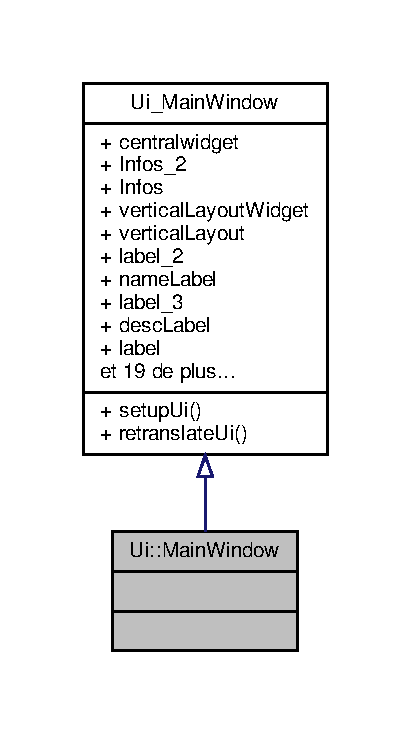
\includegraphics[width=197pt]{classUi_1_1MainWindow__inherit__graph}
\end{center}
\end{figure}


Graphe de collaboration de Ui\+:\+:Main\+Window\+:\nopagebreak
\begin{figure}[H]
\begin{center}
\leavevmode
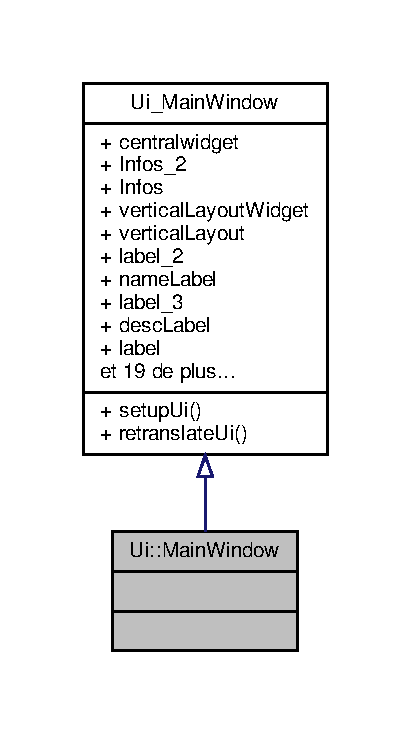
\includegraphics[width=197pt]{classUi_1_1MainWindow__coll__graph}
\end{center}
\end{figure}
\subsection*{Membres hérités additionnels}


La documentation de cette classe a été générée à partir du fichier suivant \+:\begin{DoxyCompactItemize}
\item 
\hyperlink{ui__mainwindow_8h}{ui\+\_\+mainwindow.\+h}\end{DoxyCompactItemize}

\hypertarget{classUi_1_1MainWindowLaunchDialog}{}\section{Référence de la classe Ui\+:\+:Main\+Window\+Launch\+Dialog}
\label{classUi_1_1MainWindowLaunchDialog}\index{Ui\+::\+Main\+Window\+Launch\+Dialog@{Ui\+::\+Main\+Window\+Launch\+Dialog}}


{\ttfamily \#include $<$ui\+\_\+mainwindowlaunchdialog.\+h$>$}



Graphe d\textquotesingle{}héritage de Ui\+:\+:Main\+Window\+Launch\+Dialog\+:\nopagebreak
\begin{figure}[H]
\begin{center}
\leavevmode
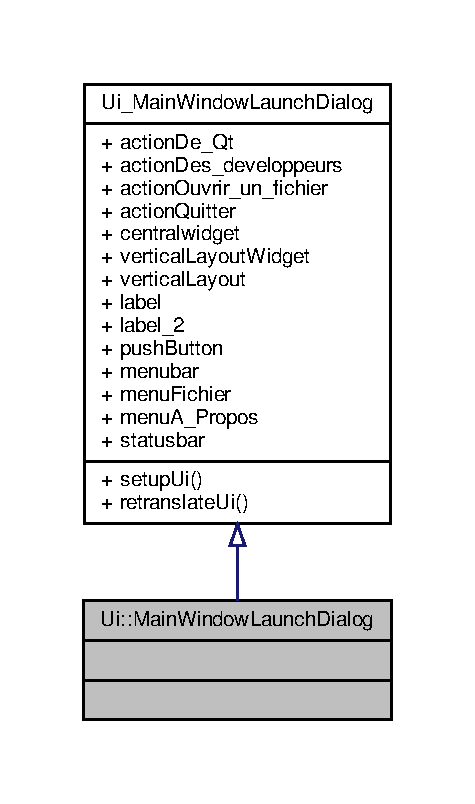
\includegraphics[width=228pt]{classUi_1_1MainWindowLaunchDialog__inherit__graph}
\end{center}
\end{figure}


Graphe de collaboration de Ui\+:\+:Main\+Window\+Launch\+Dialog\+:\nopagebreak
\begin{figure}[H]
\begin{center}
\leavevmode
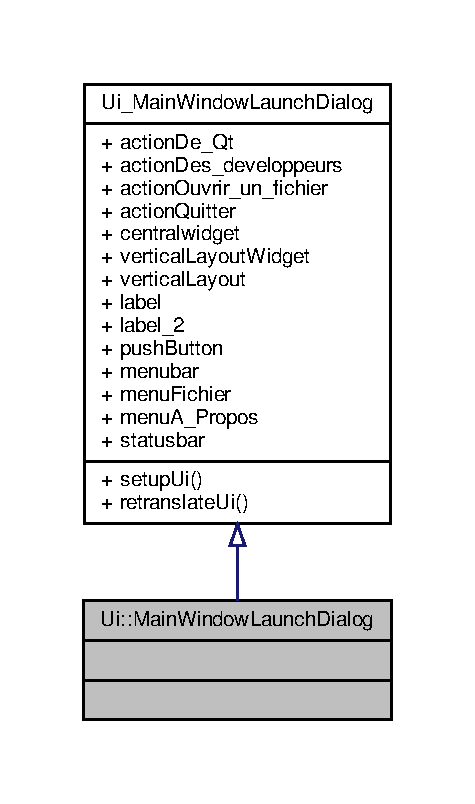
\includegraphics[width=228pt]{classUi_1_1MainWindowLaunchDialog__coll__graph}
\end{center}
\end{figure}
\subsection*{Membres hérités additionnels}


La documentation de cette classe a été générée à partir du fichier suivant \+:\begin{DoxyCompactItemize}
\item 
\hyperlink{ui__mainwindowlaunchdialog_8h}{ui\+\_\+mainwindowlaunchdialog.\+h}\end{DoxyCompactItemize}

\hypertarget{classMainWindowLaunchDialog}{}\doxysection{Main\+Window\+Launch\+Dialog Class Reference}
\label{classMainWindowLaunchDialog}\index{MainWindowLaunchDialog@{MainWindowLaunchDialog}}


{\ttfamily \#include $<$mainwindowlaunchdialog.\+h$>$}



Inheritance diagram for Main\+Window\+Launch\+Dialog\+:
\nopagebreak
\begin{figure}[H]
\begin{center}
\leavevmode
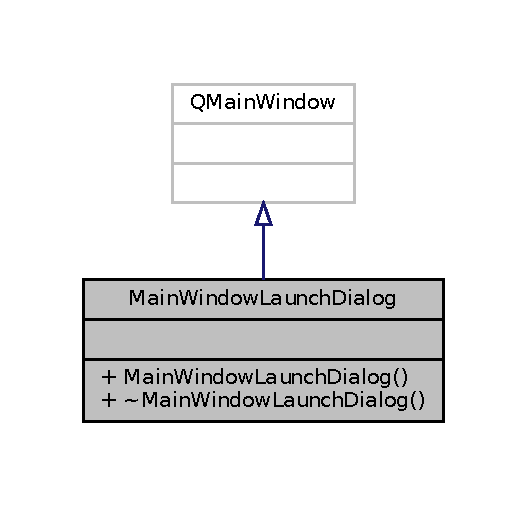
\includegraphics[width=253pt]{classMainWindowLaunchDialog__inherit__graph}
\end{center}
\end{figure}


Collaboration diagram for Main\+Window\+Launch\+Dialog\+:
\nopagebreak
\begin{figure}[H]
\begin{center}
\leavevmode
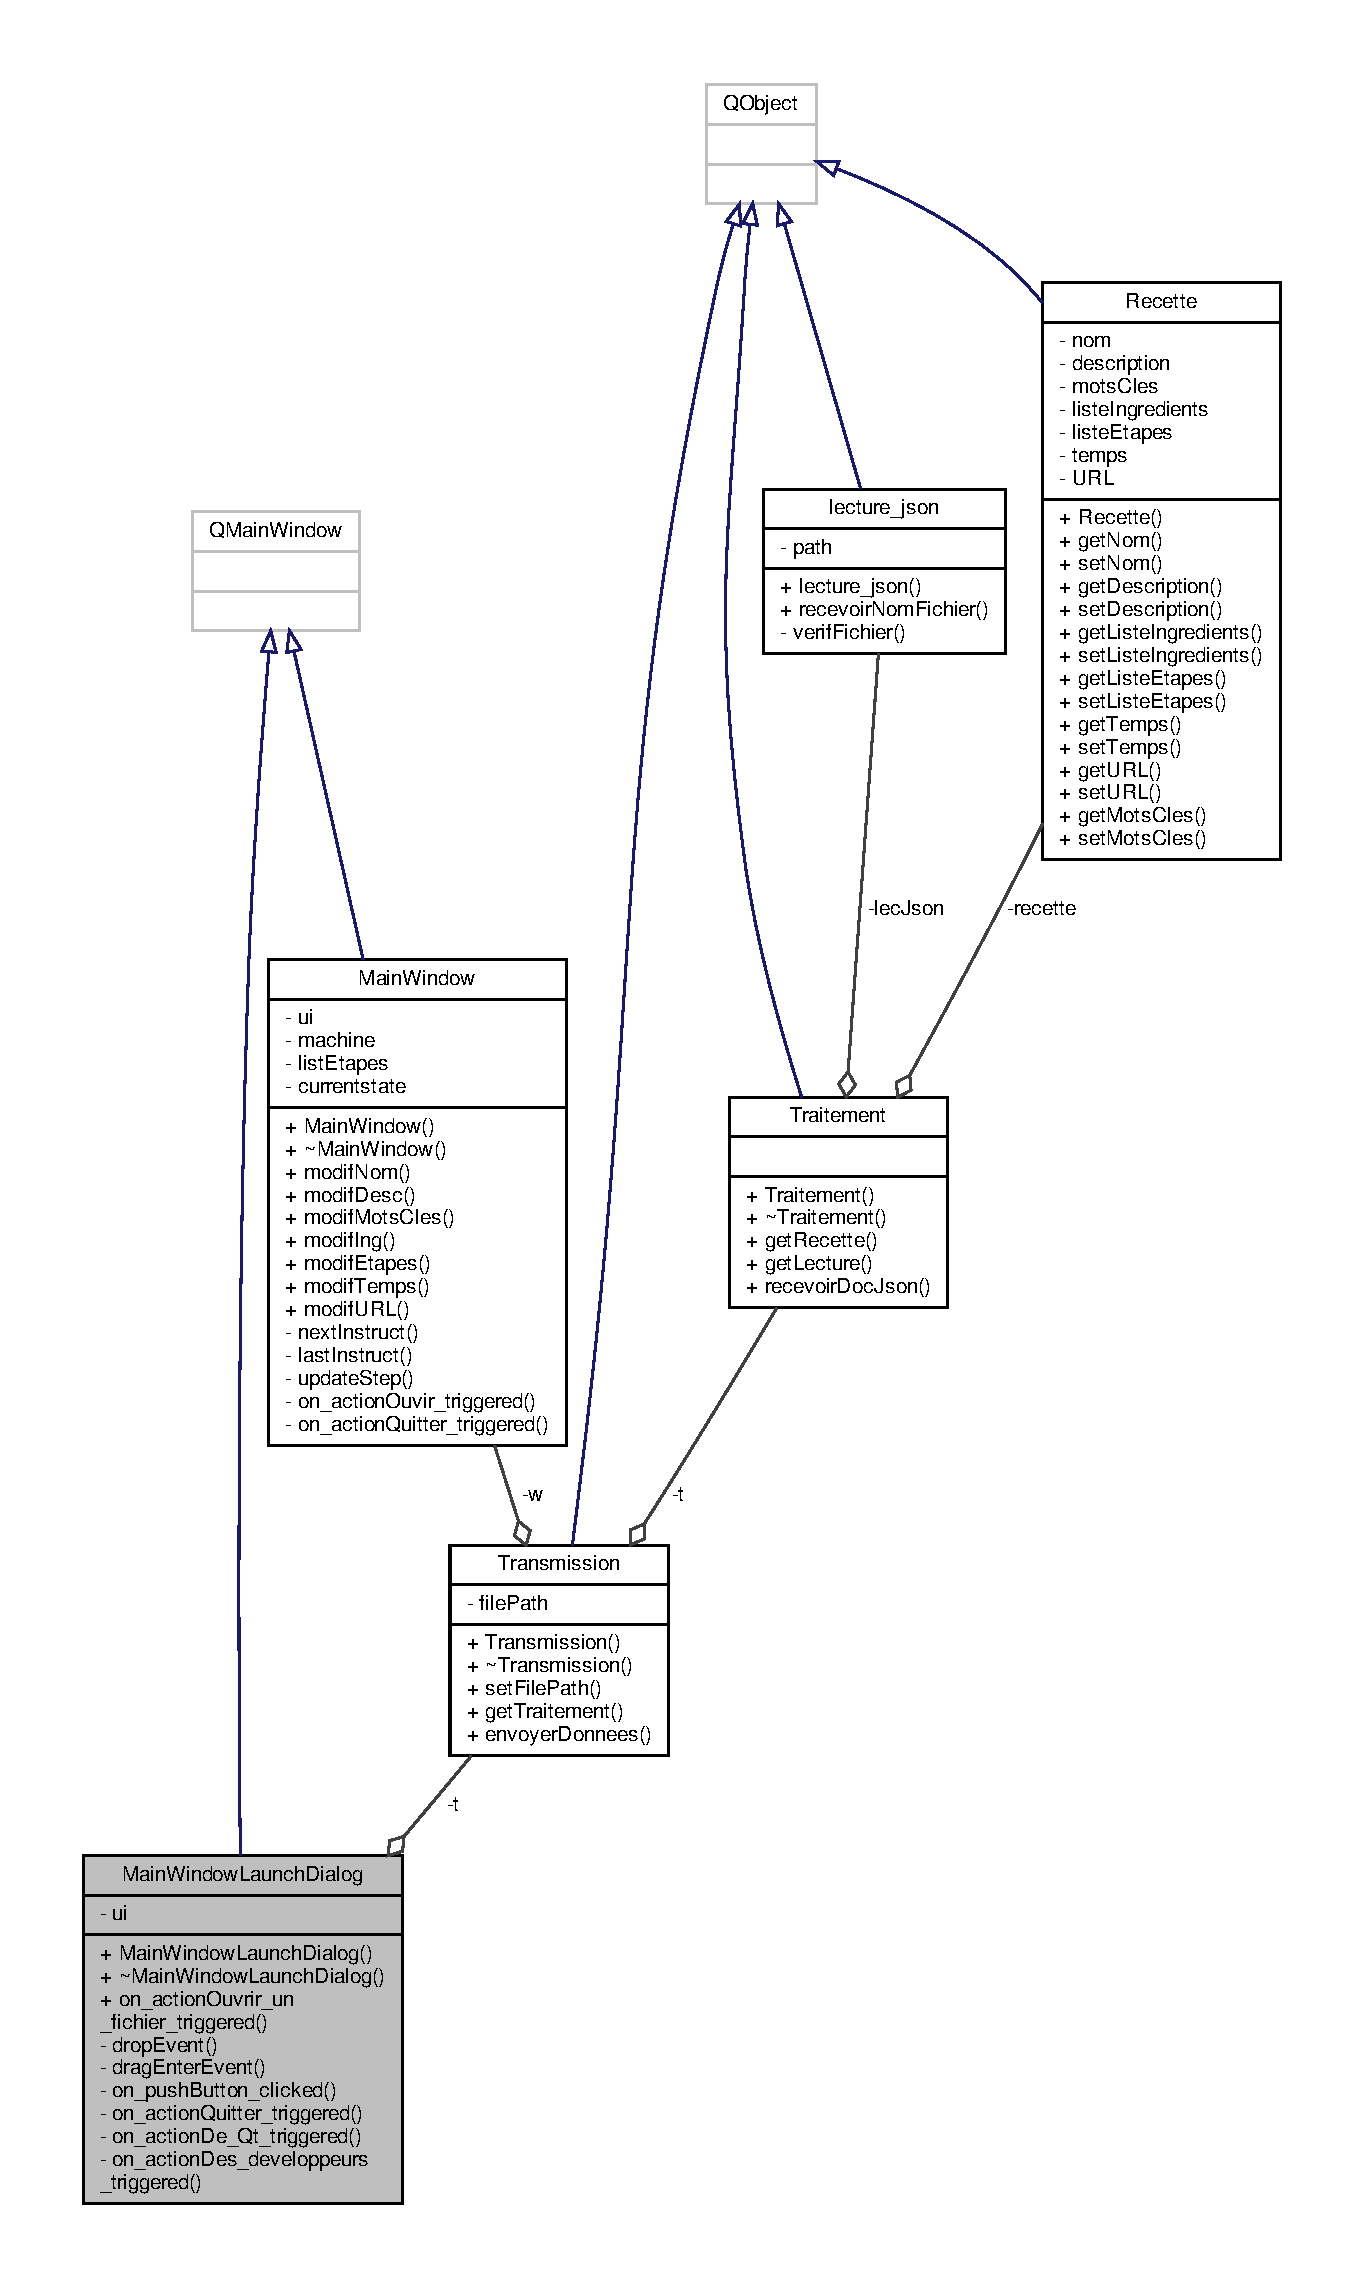
\includegraphics[width=253pt]{classMainWindowLaunchDialog__coll__graph}
\end{center}
\end{figure}
\doxysubsection*{Public Member Functions}
\begin{DoxyCompactItemize}
\item 
\mbox{\hyperlink{classMainWindowLaunchDialog_a9f7ef6d5da5eff43adb6ea835f0790d0}{Main\+Window\+Launch\+Dialog}} (Q\+Widget $\ast$parent=nullptr)
\begin{DoxyCompactList}\small\item\em Constructeur de la fenêtre de lancement. \end{DoxyCompactList}\item 
\mbox{\hyperlink{classMainWindowLaunchDialog_abf8a63fe899ba6d8fcbdf179122dfcb7}{$\sim$\+Main\+Window\+Launch\+Dialog}} ()
\begin{DoxyCompactList}\small\item\em Destructeur de la fonction \mbox{\hyperlink{classMainWindowLaunchDialog}{Main\+Window\+Launch\+Dialog}}. \end{DoxyCompactList}\end{DoxyCompactItemize}


\doxysubsection{Constructor \& Destructor Documentation}
\mbox{\Hypertarget{classMainWindowLaunchDialog_a9f7ef6d5da5eff43adb6ea835f0790d0}\label{classMainWindowLaunchDialog_a9f7ef6d5da5eff43adb6ea835f0790d0}} 
\index{MainWindowLaunchDialog@{MainWindowLaunchDialog}!MainWindowLaunchDialog@{MainWindowLaunchDialog}}
\index{MainWindowLaunchDialog@{MainWindowLaunchDialog}!MainWindowLaunchDialog@{MainWindowLaunchDialog}}
\doxysubsubsection{\texorpdfstring{MainWindowLaunchDialog()}{MainWindowLaunchDialog()}}
{\footnotesize\ttfamily Main\+Window\+Launch\+Dialog\+::\+Main\+Window\+Launch\+Dialog (\begin{DoxyParamCaption}\item[{Q\+Widget $\ast$}]{parent = {\ttfamily nullptr} }\end{DoxyParamCaption})\hspace{0.3cm}{\ttfamily [explicit]}}



Constructeur de la fenêtre de lancement. 


\begin{DoxyParams}{Parameters}
{\em Qwidget} & $\ast$parent \\
\hline
\end{DoxyParams}
\mbox{\Hypertarget{classMainWindowLaunchDialog_abf8a63fe899ba6d8fcbdf179122dfcb7}\label{classMainWindowLaunchDialog_abf8a63fe899ba6d8fcbdf179122dfcb7}} 
\index{MainWindowLaunchDialog@{MainWindowLaunchDialog}!````~MainWindowLaunchDialog@{$\sim$MainWindowLaunchDialog}}
\index{````~MainWindowLaunchDialog@{$\sim$MainWindowLaunchDialog}!MainWindowLaunchDialog@{MainWindowLaunchDialog}}
\doxysubsubsection{\texorpdfstring{$\sim$MainWindowLaunchDialog()}{~MainWindowLaunchDialog()}}
{\footnotesize\ttfamily Main\+Window\+Launch\+Dialog\+::$\sim$\+Main\+Window\+Launch\+Dialog (\begin{DoxyParamCaption}{ }\end{DoxyParamCaption})}



Destructeur de la fonction \mbox{\hyperlink{classMainWindowLaunchDialog}{Main\+Window\+Launch\+Dialog}}. 



The documentation for this class was generated from the following files\+:\begin{DoxyCompactItemize}
\item 
\mbox{\hyperlink{mainwindowlaunchdialog_8h}{mainwindowlaunchdialog.\+h}}\item 
\mbox{\hyperlink{mainwindowlaunchdialog_8cpp}{mainwindowlaunchdialog.\+cpp}}\end{DoxyCompactItemize}

\hypertarget{classRecette}{}\doxysection{Recette Class Reference}
\label{classRecette}\index{Recette@{Recette}}


Inheritance diagram for Recette\+:\nopagebreak
\begin{figure}[H]
\begin{center}
\leavevmode
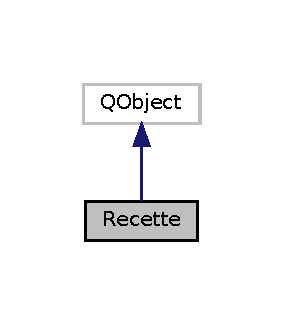
\includegraphics[width=136pt]{classRecette__inherit__graph}
\end{center}
\end{figure}


Collaboration diagram for Recette\+:\nopagebreak
\begin{figure}[H]
\begin{center}
\leavevmode
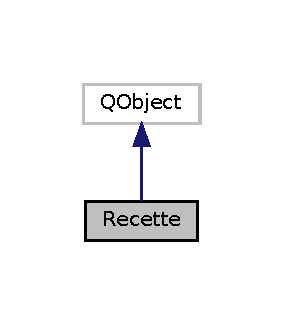
\includegraphics[width=136pt]{classRecette__coll__graph}
\end{center}
\end{figure}
\doxysubsection*{Signals}
\begin{DoxyCompactItemize}
\item 
\mbox{\Hypertarget{classRecette_aaf3e04383c78a2cef6af41eac226f07d}\label{classRecette_aaf3e04383c78a2cef6af41eac226f07d}} 
void {\bfseries envoie\+Nom} (Q\+String)
\item 
\mbox{\Hypertarget{classRecette_a4871cd68f067b53e882eb2389c11c763}\label{classRecette_a4871cd68f067b53e882eb2389c11c763}} 
void {\bfseries envoie\+Desc} (Q\+String)
\item 
\mbox{\Hypertarget{classRecette_a06b677268e4a76357a008460bf78bf57}\label{classRecette_a06b677268e4a76357a008460bf78bf57}} 
void {\bfseries envoie\+Mots\+Cles} (Q\+String)
\item 
\mbox{\Hypertarget{classRecette_a02f5f61d8c8a59b482f81da7450aa133}\label{classRecette_a02f5f61d8c8a59b482f81da7450aa133}} 
void {\bfseries envoie\+Ing} (Q\+String\+List)
\item 
\mbox{\Hypertarget{classRecette_ab8af419707ae263fb7b273988b81bd6e}\label{classRecette_ab8af419707ae263fb7b273988b81bd6e}} 
void {\bfseries envoie\+Etapes} (Q\+String\+List)
\item 
\mbox{\Hypertarget{classRecette_ad90a82b00fc7f1cc7d66ce54a3c853d8}\label{classRecette_ad90a82b00fc7f1cc7d66ce54a3c853d8}} 
void {\bfseries envoie\+Temps} (Q\+String\+List)
\item 
\mbox{\Hypertarget{classRecette_a151a21f960ad1c36b8760dee77352d99}\label{classRecette_a151a21f960ad1c36b8760dee77352d99}} 
void {\bfseries envoie\+U\+RL} (Q\+String)
\end{DoxyCompactItemize}
\doxysubsection*{Public Member Functions}
\begin{DoxyCompactItemize}
\item 
\mbox{\Hypertarget{classRecette_a23c2060e8d97d05f5f9b9178b7efdf65}\label{classRecette_a23c2060e8d97d05f5f9b9178b7efdf65}} 
{\bfseries Recette} (Q\+Object $\ast$parent=nullptr)
\item 
\mbox{\Hypertarget{classRecette_a8027ff1bf471e84d58b427e114f41467}\label{classRecette_a8027ff1bf471e84d58b427e114f41467}} 
Q\+String {\bfseries get\+Nom} () const
\item 
\mbox{\Hypertarget{classRecette_a0f0e56f6a46e7b24a4b535ae66b220e3}\label{classRecette_a0f0e56f6a46e7b24a4b535ae66b220e3}} 
void {\bfseries set\+Nom} (const Q\+String \&value)
\item 
\mbox{\Hypertarget{classRecette_acd1c8d30940dc81d5884038c7e211cd2}\label{classRecette_acd1c8d30940dc81d5884038c7e211cd2}} 
Q\+String {\bfseries get\+Description} () const
\item 
\mbox{\Hypertarget{classRecette_a503274cc926f740d676c6366b22ae798}\label{classRecette_a503274cc926f740d676c6366b22ae798}} 
void {\bfseries set\+Description} (const Q\+String \&value)
\item 
\mbox{\Hypertarget{classRecette_a2633ce9fe70a0651c7654d84e2a9dc0c}\label{classRecette_a2633ce9fe70a0651c7654d84e2a9dc0c}} 
Q\+String\+List {\bfseries get\+Liste\+Ingredients} () const
\item 
\mbox{\Hypertarget{classRecette_a17ccee7f98dbc85a1506a8398d9a435d}\label{classRecette_a17ccee7f98dbc85a1506a8398d9a435d}} 
void {\bfseries set\+Liste\+Ingredients} (const Q\+String\+List \&value)
\item 
\mbox{\Hypertarget{classRecette_a70edc43faab5130a575fcc7a0df2c7d2}\label{classRecette_a70edc43faab5130a575fcc7a0df2c7d2}} 
Q\+String\+List {\bfseries get\+Liste\+Etapes} () const
\item 
\mbox{\Hypertarget{classRecette_a375b9d966c41ab8f01b0fb998361a828}\label{classRecette_a375b9d966c41ab8f01b0fb998361a828}} 
void {\bfseries set\+Liste\+Etapes} (const Q\+String\+List \&value)
\item 
\mbox{\Hypertarget{classRecette_aa1b7f36afbb5754bb75cca86e3d82700}\label{classRecette_aa1b7f36afbb5754bb75cca86e3d82700}} 
Q\+String\+List {\bfseries get\+Temps} () const
\item 
\mbox{\Hypertarget{classRecette_a487da4eaeb42875a44b0ac6368a6f38c}\label{classRecette_a487da4eaeb42875a44b0ac6368a6f38c}} 
void {\bfseries set\+Temps} (const Q\+String\+List \&value)
\item 
\mbox{\Hypertarget{classRecette_a3fbb67f96165beb12f3726a78b0e3952}\label{classRecette_a3fbb67f96165beb12f3726a78b0e3952}} 
Q\+String {\bfseries get\+U\+RL} () const
\item 
\mbox{\Hypertarget{classRecette_afd68e52a434302e51465d1fe46f794e6}\label{classRecette_afd68e52a434302e51465d1fe46f794e6}} 
void {\bfseries set\+U\+RL} (const Q\+String \&value)
\item 
\mbox{\Hypertarget{classRecette_a6818d81767bb760afbbec5dba6fb8514}\label{classRecette_a6818d81767bb760afbbec5dba6fb8514}} 
Q\+String {\bfseries get\+Mots\+Cles} () const
\item 
\mbox{\Hypertarget{classRecette_a73602a33f2827930b2c7946f98cf11dd}\label{classRecette_a73602a33f2827930b2c7946f98cf11dd}} 
void {\bfseries set\+Mots\+Cles} (const Q\+String \&value)
\end{DoxyCompactItemize}


The documentation for this class was generated from the following files\+:\begin{DoxyCompactItemize}
\item 
\mbox{\hyperlink{recette_8h}{recette.\+h}}\item 
\mbox{\hyperlink{recette_8cpp}{recette.\+cpp}}\end{DoxyCompactItemize}

\hypertarget{classTraitement}{}\section{Référence de la classe Traitement}
\label{classTraitement}\index{Traitement@{Traitement}}


{\ttfamily \#include $<$traitement.\+h$>$}



Graphe d\textquotesingle{}héritage de Traitement\+:\nopagebreak
\begin{figure}[H]
\begin{center}
\leavevmode
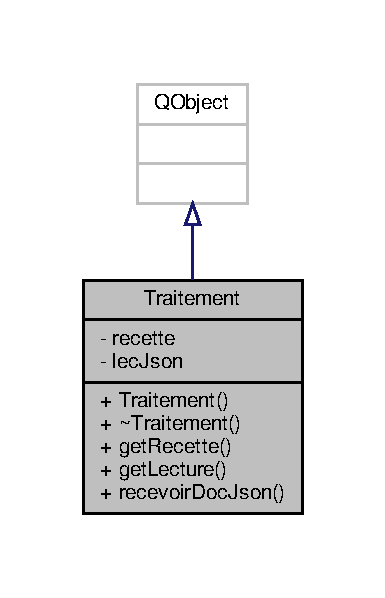
\includegraphics[width=185pt]{classTraitement__inherit__graph}
\end{center}
\end{figure}


Graphe de collaboration de Traitement\+:\nopagebreak
\begin{figure}[H]
\begin{center}
\leavevmode
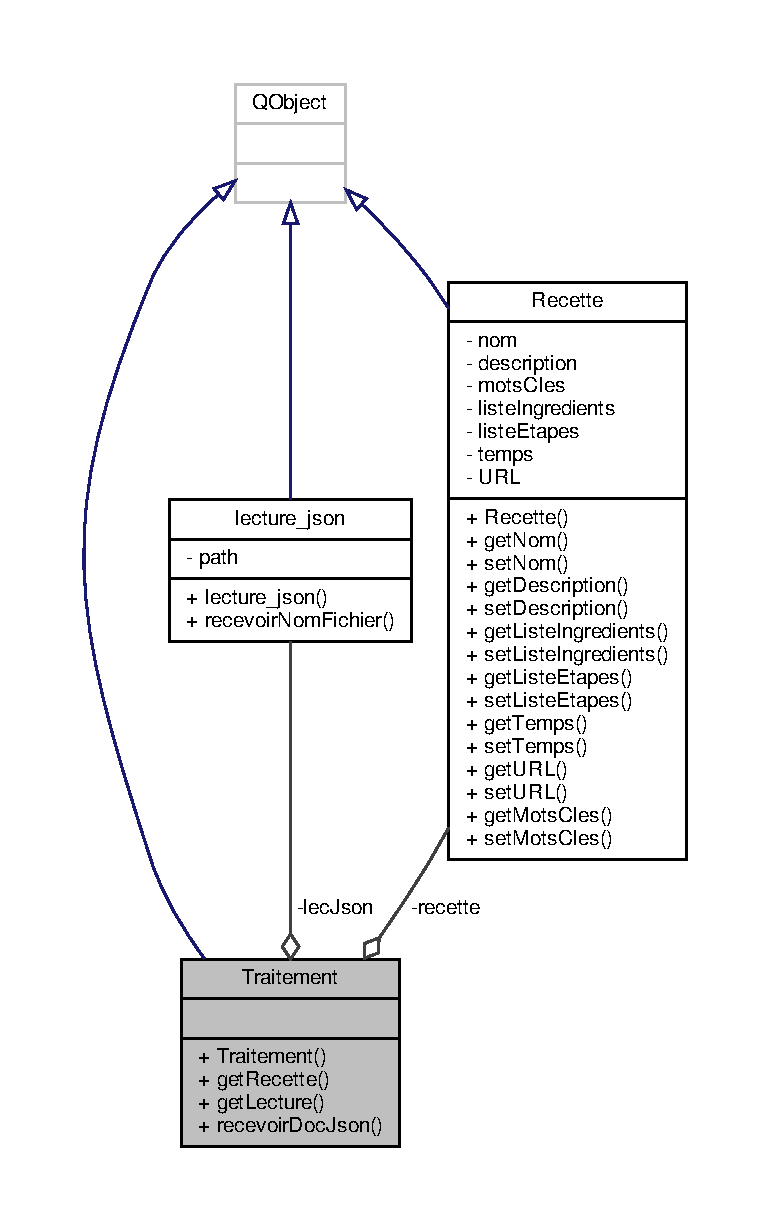
\includegraphics[height=550pt]{classTraitement__coll__graph}
\end{center}
\end{figure}
\subsection*{Connecteurs publics}
\begin{DoxyCompactItemize}
\item 
void \hyperlink{classTraitement_a7bbc7e2034b55a9de14c010be7d3de11}{recevoir\+Doc\+Json} (Q\+Json\+Document doc\+Json)
\begin{DoxyCompactList}\small\item\em fonction qui recoit le document J\+S\+ON pour le traiter et lire ses données \end{DoxyCompactList}\end{DoxyCompactItemize}
\subsection*{Signaux}
\begin{DoxyCompactItemize}
\item 
void \hyperlink{classTraitement_a9f84743a77b0074f209eda21d32ee95b}{envoie\+Nom} (Q\+String nom)
\begin{DoxyCompactList}\small\item\em Fonction (signal) pour envoyer le nom à la classe \hyperlink{classMainWindow}{Main\+Window} (voir classe \hyperlink{classMainWindow}{Main\+Window}) \end{DoxyCompactList}\item 
void \hyperlink{classTraitement_a81d1717924fb7a206df394afae4e19dc}{envoie\+Desc} (Q\+String)
\begin{DoxyCompactList}\small\item\em Fonction (signal) pour envoyer la description à la classe \hyperlink{classMainWindow}{Main\+Window} (voir classe \hyperlink{classMainWindow}{Main\+Window}) \end{DoxyCompactList}\item 
void \hyperlink{classTraitement_a4df691c4f46371e6c2b6b4c4df102819}{envoie\+Mots\+Cles} (Q\+String)
\begin{DoxyCompactList}\small\item\em fonction (signal) pour envoyer les mots cles à la classe \hyperlink{classMainWindow}{Main\+Window} (voir classe \hyperlink{classMainWindow}{Main\+Window}) \end{DoxyCompactList}\item 
void \hyperlink{classTraitement_a8db23635eb895875b0f60acece723df4}{envoie\+Ing} (Q\+String\+List)
\begin{DoxyCompactList}\small\item\em fonction (signal) pour envoyer la liste des ingrédients à la classe \hyperlink{classMainWindow}{Main\+Window} (voir classe \hyperlink{classMainWindow}{Main\+Window}) \end{DoxyCompactList}\item 
void \hyperlink{classTraitement_ae58a2b32e2632bfc11a696c186ace3b7}{envoie\+Etapes} (Q\+String\+List)
\begin{DoxyCompactList}\small\item\em fonction (signal) pour envoyer la liste des étapes à la classe \hyperlink{classMainWindow}{Main\+Window} (voir classe \hyperlink{classMainWindow}{Main\+Window}) \end{DoxyCompactList}\item 
void \hyperlink{classTraitement_ae57543af34e05b74a7af460c0e74e87f}{envoie\+Temps} (Q\+String)
\begin{DoxyCompactList}\small\item\em fonction (signal) pour envoyer les temps à la classe \hyperlink{classMainWindow}{Main\+Window} (voir classe \hyperlink{classMainWindow}{Main\+Window}) \end{DoxyCompactList}\item 
void \hyperlink{classTraitement_acc099bf1113669c2e061e8897c3eaeca}{envoie\+U\+RL} (Q\+String)
\begin{DoxyCompactList}\small\item\em fonction (signal) pour envoyer l\textquotesingle{}url à la classe \hyperlink{classMainWindow}{Main\+Window} (voir classe \hyperlink{classMainWindow}{Main\+Window}) \end{DoxyCompactList}\item 
void \hyperlink{classTraitement_a83495c6e878e66511b8af67ee369a012}{fin\+Traitement} ()
\begin{DoxyCompactList}\small\item\em Fonction (signal) pour envoyer le chemin du fichier. \end{DoxyCompactList}\end{DoxyCompactItemize}
\subsection*{Fonctions membres publiques}
\begin{DoxyCompactItemize}
\item 
\hyperlink{classTraitement_a36edd9e6ce6e72cfef7f9c857c3c9cf2}{Traitement} (Q\+Object $\ast$parent=nullptr)
\begin{DoxyCompactList}\small\item\em Constructeur de la classe \hyperlink{classTraitement}{Traitement}. \end{DoxyCompactList}\item 
\hyperlink{classTraitement_a7dd82f97c992d07b7032184f12c7fab9}{$\sim$\+Traitement} ()
\begin{DoxyCompactList}\small\item\em Destructeur de la classe \hyperlink{classTraitement}{Traitement}. \end{DoxyCompactList}\item 
\hyperlink{classRecette}{Recette} $\ast$ \hyperlink{classTraitement_a587f76ba51e61307815c9e279821a744}{get\+Recette} ()
\begin{DoxyCompactList}\small\item\em Fonction getter pour obtenir l\textquotesingle{}instance de la classe \hyperlink{classRecette}{Recette}. \end{DoxyCompactList}\item 
\hyperlink{classlecture__json}{lecture\+\_\+json} $\ast$ \hyperlink{classTraitement_a91ecaaa93bbdc283a3eebe3c060e656d}{get\+Lecture} ()
\begin{DoxyCompactList}\small\item\em Fonction getter pour obtenir l\textquotesingle{}instance de la classe \hyperlink{classlecture__json}{lecture\+\_\+json}. \end{DoxyCompactList}\end{DoxyCompactItemize}
\subsection*{Attributs privés}
\begin{DoxyCompactItemize}
\item 
\hyperlink{classRecette}{Recette} $\ast$ \hyperlink{classTraitement_afc8ac78bded6d17a86323544aa00d91b}{recette}
\item 
\hyperlink{classlecture__json}{lecture\+\_\+json} $\ast$ \hyperlink{classTraitement_ac7e6ff3bfc54975b1c8831a2ad8fc9a4}{lec\+Json}
\end{DoxyCompactItemize}


\subsection{Documentation des constructeurs et destructeur}
\mbox{\Hypertarget{classTraitement_a36edd9e6ce6e72cfef7f9c857c3c9cf2}\label{classTraitement_a36edd9e6ce6e72cfef7f9c857c3c9cf2}} 
\index{Traitement@{Traitement}!Traitement@{Traitement}}
\index{Traitement@{Traitement}!Traitement@{Traitement}}
\subsubsection{\texorpdfstring{Traitement()}{Traitement()}}
{\footnotesize\ttfamily Traitement\+::\+Traitement (\begin{DoxyParamCaption}\item[{Q\+Object $\ast$}]{parent = {\ttfamily nullptr} }\end{DoxyParamCaption})\hspace{0.3cm}{\ttfamily [explicit]}}



Constructeur de la classe \hyperlink{classTraitement}{Traitement}. 


\begin{DoxyParams}{Paramètres}
{\em parent} & \+: précise si le widget hérite d\textquotesingle{}une autre fenêtre \\
\hline
\end{DoxyParams}
\mbox{\Hypertarget{classTraitement_a7dd82f97c992d07b7032184f12c7fab9}\label{classTraitement_a7dd82f97c992d07b7032184f12c7fab9}} 
\index{Traitement@{Traitement}!````~Traitement@{$\sim$\+Traitement}}
\index{````~Traitement@{$\sim$\+Traitement}!Traitement@{Traitement}}
\subsubsection{\texorpdfstring{$\sim$\+Traitement()}{~Traitement()}}
{\footnotesize\ttfamily Traitement\+::$\sim$\+Traitement (\begin{DoxyParamCaption}{ }\end{DoxyParamCaption})}



Destructeur de la classe \hyperlink{classTraitement}{Traitement}. 



\subsection{Documentation des fonctions membres}
\mbox{\Hypertarget{classTraitement_a81d1717924fb7a206df394afae4e19dc}\label{classTraitement_a81d1717924fb7a206df394afae4e19dc}} 
\index{Traitement@{Traitement}!envoie\+Desc@{envoie\+Desc}}
\index{envoie\+Desc@{envoie\+Desc}!Traitement@{Traitement}}
\subsubsection{\texorpdfstring{envoie\+Desc}{envoieDesc}}
{\footnotesize\ttfamily void Traitement\+::envoie\+Desc (\begin{DoxyParamCaption}\item[{Q\+String}]{ }\end{DoxyParamCaption})\hspace{0.3cm}{\ttfamily [signal]}}



Fonction (signal) pour envoyer la description à la classe \hyperlink{classMainWindow}{Main\+Window} (voir classe \hyperlink{classMainWindow}{Main\+Window}) 

\begin{DoxySeeAlso}{Voir également}
\hyperlink{classTraitement_a81d1717924fb7a206df394afae4e19dc}{envoie\+Desc(\+Q\+String)} 
\end{DoxySeeAlso}

\begin{DoxyParams}{Paramètres}
{\em desc} & \+: la description à transmettre \\
\hline
\end{DoxyParams}
\mbox{\Hypertarget{classTraitement_ae58a2b32e2632bfc11a696c186ace3b7}\label{classTraitement_ae58a2b32e2632bfc11a696c186ace3b7}} 
\index{Traitement@{Traitement}!envoie\+Etapes@{envoie\+Etapes}}
\index{envoie\+Etapes@{envoie\+Etapes}!Traitement@{Traitement}}
\subsubsection{\texorpdfstring{envoie\+Etapes}{envoieEtapes}}
{\footnotesize\ttfamily void Traitement\+::envoie\+Etapes (\begin{DoxyParamCaption}\item[{Q\+String\+List}]{ }\end{DoxyParamCaption})\hspace{0.3cm}{\ttfamily [signal]}}



fonction (signal) pour envoyer la liste des étapes à la classe \hyperlink{classMainWindow}{Main\+Window} (voir classe \hyperlink{classMainWindow}{Main\+Window}) 

\begin{DoxySeeAlso}{Voir également}
\hyperlink{classTraitement_ae58a2b32e2632bfc11a696c186ace3b7}{envoie\+Etapes(\+Q\+String\+List)} 
\end{DoxySeeAlso}

\begin{DoxyParams}{Paramètres}
{\em étapes} & \+: la liste des étapes à transmettre \\
\hline
\end{DoxyParams}
\mbox{\Hypertarget{classTraitement_a8db23635eb895875b0f60acece723df4}\label{classTraitement_a8db23635eb895875b0f60acece723df4}} 
\index{Traitement@{Traitement}!envoie\+Ing@{envoie\+Ing}}
\index{envoie\+Ing@{envoie\+Ing}!Traitement@{Traitement}}
\subsubsection{\texorpdfstring{envoie\+Ing}{envoieIng}}
{\footnotesize\ttfamily void Traitement\+::envoie\+Ing (\begin{DoxyParamCaption}\item[{Q\+String\+List}]{ }\end{DoxyParamCaption})\hspace{0.3cm}{\ttfamily [signal]}}



fonction (signal) pour envoyer la liste des ingrédients à la classe \hyperlink{classMainWindow}{Main\+Window} (voir classe \hyperlink{classMainWindow}{Main\+Window}) 

\begin{DoxySeeAlso}{Voir également}
\hyperlink{classTraitement_a8db23635eb895875b0f60acece723df4}{envoie\+Ing(\+Q\+String\+List)} 
\end{DoxySeeAlso}

\begin{DoxyParams}{Paramètres}
{\em ingredients} & \+: la liste des ingrédients à transmettre \\
\hline
\end{DoxyParams}
\mbox{\Hypertarget{classTraitement_a4df691c4f46371e6c2b6b4c4df102819}\label{classTraitement_a4df691c4f46371e6c2b6b4c4df102819}} 
\index{Traitement@{Traitement}!envoie\+Mots\+Cles@{envoie\+Mots\+Cles}}
\index{envoie\+Mots\+Cles@{envoie\+Mots\+Cles}!Traitement@{Traitement}}
\subsubsection{\texorpdfstring{envoie\+Mots\+Cles}{envoieMotsCles}}
{\footnotesize\ttfamily void Traitement\+::envoie\+Mots\+Cles (\begin{DoxyParamCaption}\item[{Q\+String}]{ }\end{DoxyParamCaption})\hspace{0.3cm}{\ttfamily [signal]}}



fonction (signal) pour envoyer les mots cles à la classe \hyperlink{classMainWindow}{Main\+Window} (voir classe \hyperlink{classMainWindow}{Main\+Window}) 

\begin{DoxySeeAlso}{Voir également}
\hyperlink{classTraitement_a4df691c4f46371e6c2b6b4c4df102819}{envoie\+Mots\+Cles(\+Q\+String)} 
\end{DoxySeeAlso}

\begin{DoxyParams}{Paramètres}
{\em Mots\+Cles} & les mots cles à transmettre \\
\hline
\end{DoxyParams}
\mbox{\Hypertarget{classTraitement_a9f84743a77b0074f209eda21d32ee95b}\label{classTraitement_a9f84743a77b0074f209eda21d32ee95b}} 
\index{Traitement@{Traitement}!envoie\+Nom@{envoie\+Nom}}
\index{envoie\+Nom@{envoie\+Nom}!Traitement@{Traitement}}
\subsubsection{\texorpdfstring{envoie\+Nom}{envoieNom}}
{\footnotesize\ttfamily void Traitement\+::envoie\+Nom (\begin{DoxyParamCaption}\item[{Q\+String}]{nom }\end{DoxyParamCaption})\hspace{0.3cm}{\ttfamily [signal]}}



Fonction (signal) pour envoyer le nom à la classe \hyperlink{classMainWindow}{Main\+Window} (voir classe \hyperlink{classMainWindow}{Main\+Window}) 

\begin{DoxySeeAlso}{Voir également}
\hyperlink{classTraitement_a9f84743a77b0074f209eda21d32ee95b}{envoie\+Nom(\+Q\+String)} 
\end{DoxySeeAlso}

\begin{DoxyParams}{Paramètres}
{\em nom} & le nom à transmettre \\
\hline
\end{DoxyParams}
\mbox{\Hypertarget{classTraitement_ae57543af34e05b74a7af460c0e74e87f}\label{classTraitement_ae57543af34e05b74a7af460c0e74e87f}} 
\index{Traitement@{Traitement}!envoie\+Temps@{envoie\+Temps}}
\index{envoie\+Temps@{envoie\+Temps}!Traitement@{Traitement}}
\subsubsection{\texorpdfstring{envoie\+Temps}{envoieTemps}}
{\footnotesize\ttfamily void Traitement\+::envoie\+Temps (\begin{DoxyParamCaption}\item[{Q\+String}]{ }\end{DoxyParamCaption})\hspace{0.3cm}{\ttfamily [signal]}}



fonction (signal) pour envoyer les temps à la classe \hyperlink{classMainWindow}{Main\+Window} (voir classe \hyperlink{classMainWindow}{Main\+Window}) 

\begin{DoxySeeAlso}{Voir également}
\hyperlink{classTraitement_ae57543af34e05b74a7af460c0e74e87f}{envoie\+Temps(\+Q\+String)} 
\end{DoxySeeAlso}

\begin{DoxyParams}{Paramètres}
{\em temps} & \+: les temps à transmettre \\
\hline
\end{DoxyParams}
\mbox{\Hypertarget{classTraitement_acc099bf1113669c2e061e8897c3eaeca}\label{classTraitement_acc099bf1113669c2e061e8897c3eaeca}} 
\index{Traitement@{Traitement}!envoie\+U\+RL@{envoie\+U\+RL}}
\index{envoie\+U\+RL@{envoie\+U\+RL}!Traitement@{Traitement}}
\subsubsection{\texorpdfstring{envoie\+U\+RL}{envoieURL}}
{\footnotesize\ttfamily void Traitement\+::envoie\+U\+RL (\begin{DoxyParamCaption}\item[{Q\+String}]{ }\end{DoxyParamCaption})\hspace{0.3cm}{\ttfamily [signal]}}



fonction (signal) pour envoyer l\textquotesingle{}url à la classe \hyperlink{classMainWindow}{Main\+Window} (voir classe \hyperlink{classMainWindow}{Main\+Window}) 

\begin{DoxySeeAlso}{Voir également}
\hyperlink{classTraitement_acc099bf1113669c2e061e8897c3eaeca}{envoie\+U\+R\+L(\+Q\+String)} 
\end{DoxySeeAlso}

\begin{DoxyParams}{Paramètres}
{\em url} & \+: l\textquotesingle{}url du site web de la recette à transmettre \\
\hline
\end{DoxyParams}
\mbox{\Hypertarget{classTraitement_a83495c6e878e66511b8af67ee369a012}\label{classTraitement_a83495c6e878e66511b8af67ee369a012}} 
\index{Traitement@{Traitement}!fin\+Traitement@{fin\+Traitement}}
\index{fin\+Traitement@{fin\+Traitement}!Traitement@{Traitement}}
\subsubsection{\texorpdfstring{fin\+Traitement}{finTraitement}}
{\footnotesize\ttfamily void Traitement\+::fin\+Traitement (\begin{DoxyParamCaption}{ }\end{DoxyParamCaption})\hspace{0.3cm}{\ttfamily [signal]}}



Fonction (signal) pour envoyer le chemin du fichier. 

\begin{DoxySeeAlso}{Voir également}
envoie\+Nom\+Fichier(\+Q\+String) 
\end{DoxySeeAlso}

\begin{DoxyParams}{Paramètres}
{\em Q\+String} & \+: le chemin d\textquotesingle{}accès du fichier \\
\hline
\end{DoxyParams}
\mbox{\Hypertarget{classTraitement_a91ecaaa93bbdc283a3eebe3c060e656d}\label{classTraitement_a91ecaaa93bbdc283a3eebe3c060e656d}} 
\index{Traitement@{Traitement}!get\+Lecture@{get\+Lecture}}
\index{get\+Lecture@{get\+Lecture}!Traitement@{Traitement}}
\subsubsection{\texorpdfstring{get\+Lecture()}{getLecture()}}
{\footnotesize\ttfamily Traitement\+::get\+Lecture (\begin{DoxyParamCaption}{ }\end{DoxyParamCaption})\hspace{0.3cm}{\ttfamily [inline]}}



Fonction getter pour obtenir l\textquotesingle{}instance de la classe \hyperlink{classlecture__json}{lecture\+\_\+json}. 

\begin{DoxyReturn}{Renvoie}
Un pointeur sur \hyperlink{classlecture__json}{lecture\+\_\+json} 
\end{DoxyReturn}
\mbox{\Hypertarget{classTraitement_a587f76ba51e61307815c9e279821a744}\label{classTraitement_a587f76ba51e61307815c9e279821a744}} 
\index{Traitement@{Traitement}!get\+Recette@{get\+Recette}}
\index{get\+Recette@{get\+Recette}!Traitement@{Traitement}}
\subsubsection{\texorpdfstring{get\+Recette()}{getRecette()}}
{\footnotesize\ttfamily Traitement\+::get\+Recette (\begin{DoxyParamCaption}{ }\end{DoxyParamCaption})\hspace{0.3cm}{\ttfamily [inline]}}



Fonction getter pour obtenir l\textquotesingle{}instance de la classe \hyperlink{classRecette}{Recette}. 

\begin{DoxyReturn}{Renvoie}
Un pointeur sur \hyperlink{classRecette}{Recette} 
\end{DoxyReturn}
\mbox{\Hypertarget{classTraitement_a7bbc7e2034b55a9de14c010be7d3de11}\label{classTraitement_a7bbc7e2034b55a9de14c010be7d3de11}} 
\index{Traitement@{Traitement}!recevoir\+Doc\+Json@{recevoir\+Doc\+Json}}
\index{recevoir\+Doc\+Json@{recevoir\+Doc\+Json}!Traitement@{Traitement}}
\subsubsection{\texorpdfstring{recevoir\+Doc\+Json}{recevoirDocJson}}
{\footnotesize\ttfamily void Traitement\+::recevoir\+Doc\+Json (\begin{DoxyParamCaption}\item[{Q\+Json\+Document}]{doc\+Json }\end{DoxyParamCaption})\hspace{0.3cm}{\ttfamily [slot]}}



fonction qui recoit le document J\+S\+ON pour le traiter et lire ses données 

\begin{DoxySeeAlso}{Voir également}
recevoir\+Doc\+Json(\+Q\+String) 
\end{DoxySeeAlso}

\begin{DoxyParams}{Paramètres}
{\em doc\+Json} & \+:le document J\+S\+ON à traiter \\
\hline
\end{DoxyParams}


\subsection{Documentation des données membres}
\mbox{\Hypertarget{classTraitement_ac7e6ff3bfc54975b1c8831a2ad8fc9a4}\label{classTraitement_ac7e6ff3bfc54975b1c8831a2ad8fc9a4}} 
\index{Traitement@{Traitement}!lec\+Json@{lec\+Json}}
\index{lec\+Json@{lec\+Json}!Traitement@{Traitement}}
\subsubsection{\texorpdfstring{lec\+Json}{lecJson}}
{\footnotesize\ttfamily \hyperlink{classlecture__json}{lecture\+\_\+json}$\ast$ Traitement\+::lec\+Json\hspace{0.3cm}{\ttfamily [private]}}

Mainwindow $\ast$w\+: pointeur sur la fenetre principale \mbox{\Hypertarget{classTraitement_afc8ac78bded6d17a86323544aa00d91b}\label{classTraitement_afc8ac78bded6d17a86323544aa00d91b}} 
\index{Traitement@{Traitement}!recette@{recette}}
\index{recette@{recette}!Traitement@{Traitement}}
\subsubsection{\texorpdfstring{recette}{recette}}
{\footnotesize\ttfamily \hyperlink{classRecette}{Recette}$\ast$ Traitement\+::recette\hspace{0.3cm}{\ttfamily [private]}}

\hyperlink{classRecette}{Recette} $\ast$recette\+: pointeur sur la variable recette 

La documentation de cette classe a été générée à partir des fichiers suivants \+:\begin{DoxyCompactItemize}
\item 
\hyperlink{traitement_8h}{traitement.\+h}\item 
\hyperlink{traitement_8cpp}{traitement.\+cpp}\end{DoxyCompactItemize}

\hypertarget{classTransmission}{}\section{Référence de la classe Transmission}
\label{classTransmission}\index{Transmission@{Transmission}}


{\ttfamily \#include $<$transmission.\+h$>$}



Graphe d\textquotesingle{}héritage de Transmission\+:\nopagebreak
\begin{figure}[H]
\begin{center}
\leavevmode
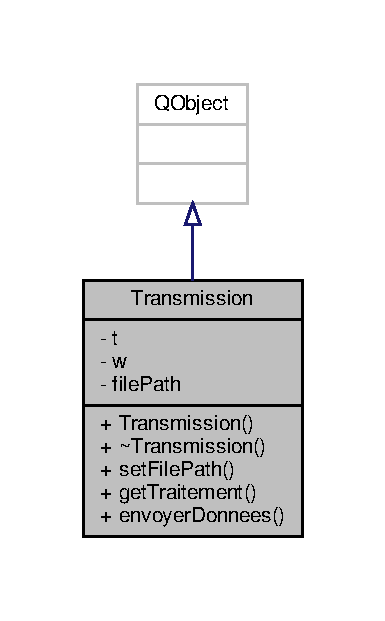
\includegraphics[width=185pt]{classTransmission__inherit__graph}
\end{center}
\end{figure}


Graphe de collaboration de Transmission\+:\nopagebreak
\begin{figure}[H]
\begin{center}
\leavevmode
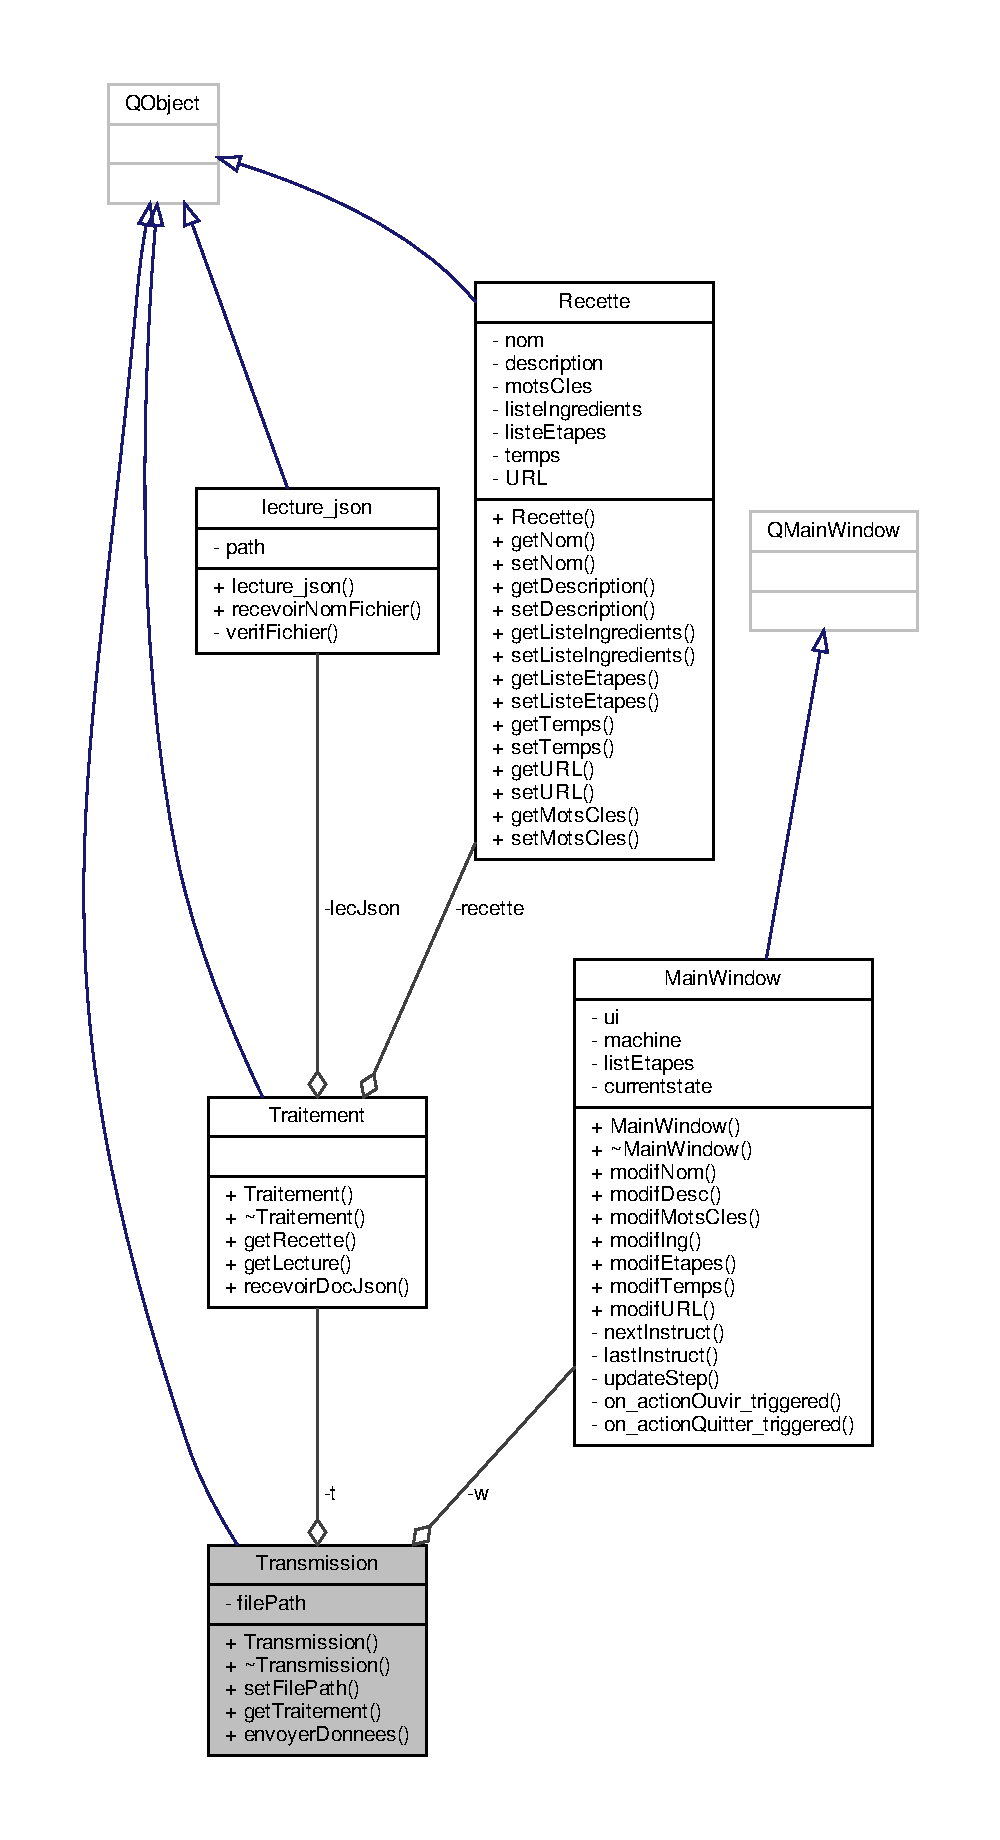
\includegraphics[height=550pt]{classTransmission__coll__graph}
\end{center}
\end{figure}
\subsection*{Connecteurs publics}
\begin{DoxyCompactItemize}
\item 
void \hyperlink{classTransmission_a14b885539e973a158c9c4c25fd99bc04}{envoyer\+Donnees} ()
\begin{DoxyCompactList}\small\item\em Fonction qui envoie les attributes de la classe \hyperlink{classRecette}{Recette} à la \hyperlink{classMainWindow}{Main\+Window}. \end{DoxyCompactList}\end{DoxyCompactItemize}
\subsection*{Fonctions membres publiques}
\begin{DoxyCompactItemize}
\item 
\hyperlink{classTransmission_a1d8087d2d09b9ddd4fd6e8261daed9f3}{Transmission} (Q\+Object $\ast$parent=nullptr)
\begin{DoxyCompactList}\small\item\em Constructeur de la fonction \hyperlink{classTransmission}{Transmission}. \end{DoxyCompactList}\item 
\hyperlink{classTransmission_adcdc6012d99ddb1d0c3159d50984e146}{$\sim$\+Transmission} ()
\begin{DoxyCompactList}\small\item\em Destructeur de la fonction \hyperlink{classTransmission}{Transmission}. \end{DoxyCompactList}\item 
void \hyperlink{classTransmission_a5099a8d2ae60a2f159230bf81bafebdc}{set\+File\+Path} (Q\+String \+\_\+file\+Path)
\begin{DoxyCompactList}\small\item\em Fonction qui permet de définir le chemin du fichier. \end{DoxyCompactList}\item 
\hyperlink{classTraitement}{Traitement} $\ast$ \hyperlink{classTransmission_ae7c158b2d20256c381d7e0bb8552f154}{get\+Traitement} ()
\begin{DoxyCompactList}\small\item\em Fonction getter pour obtenir l\textquotesingle{}instance de la classe \hyperlink{classTraitement}{Traitement}. \end{DoxyCompactList}\end{DoxyCompactItemize}
\subsection*{Attributs privés}
\begin{DoxyCompactItemize}
\item 
\hyperlink{classTraitement}{Traitement} $\ast$ \hyperlink{classTransmission_ad05ceda47dcb0763e32e03e089defdb0}{t}
\item 
\hyperlink{classMainWindow}{Main\+Window} $\ast$ \hyperlink{classTransmission_a46ff40b83d046581408dce2027139fe0}{w}
\item 
Q\+String \hyperlink{classTransmission_a3514cc6116b900b586f8cbf194cb39e7}{file\+Path} =\char`\"{}\char`\"{}
\end{DoxyCompactItemize}


\subsection{Documentation des constructeurs et destructeur}
\mbox{\Hypertarget{classTransmission_a1d8087d2d09b9ddd4fd6e8261daed9f3}\label{classTransmission_a1d8087d2d09b9ddd4fd6e8261daed9f3}} 
\index{Transmission@{Transmission}!Transmission@{Transmission}}
\index{Transmission@{Transmission}!Transmission@{Transmission}}
\subsubsection{\texorpdfstring{Transmission()}{Transmission()}}
{\footnotesize\ttfamily Transmission\+::\+Transmission (\begin{DoxyParamCaption}\item[{Q\+Object $\ast$}]{parent = {\ttfamily nullptr} }\end{DoxyParamCaption})\hspace{0.3cm}{\ttfamily [explicit]}}



Constructeur de la fonction \hyperlink{classTransmission}{Transmission}. 


\begin{DoxyParams}{Paramètres}
{\em parent} & précise si le widget hérite d\textquotesingle{}un autre object \\
\hline
\end{DoxyParams}
\mbox{\Hypertarget{classTransmission_adcdc6012d99ddb1d0c3159d50984e146}\label{classTransmission_adcdc6012d99ddb1d0c3159d50984e146}} 
\index{Transmission@{Transmission}!````~Transmission@{$\sim$\+Transmission}}
\index{````~Transmission@{$\sim$\+Transmission}!Transmission@{Transmission}}
\subsubsection{\texorpdfstring{$\sim$\+Transmission()}{~Transmission()}}
{\footnotesize\ttfamily Transmission\+::$\sim$\+Transmission (\begin{DoxyParamCaption}{ }\end{DoxyParamCaption})}



Destructeur de la fonction \hyperlink{classTransmission}{Transmission}. 



\subsection{Documentation des fonctions membres}
\mbox{\Hypertarget{classTransmission_a14b885539e973a158c9c4c25fd99bc04}\label{classTransmission_a14b885539e973a158c9c4c25fd99bc04}} 
\index{Transmission@{Transmission}!envoyer\+Donnees@{envoyer\+Donnees}}
\index{envoyer\+Donnees@{envoyer\+Donnees}!Transmission@{Transmission}}
\subsubsection{\texorpdfstring{envoyer\+Donnees}{envoyerDonnees}}
{\footnotesize\ttfamily void Transmission\+::envoyer\+Donnees (\begin{DoxyParamCaption}{ }\end{DoxyParamCaption})\hspace{0.3cm}{\ttfamily [slot]}}



Fonction qui envoie les attributes de la classe \hyperlink{classRecette}{Recette} à la \hyperlink{classMainWindow}{Main\+Window}. 

\mbox{\Hypertarget{classTransmission_ae7c158b2d20256c381d7e0bb8552f154}\label{classTransmission_ae7c158b2d20256c381d7e0bb8552f154}} 
\index{Transmission@{Transmission}!get\+Traitement@{get\+Traitement}}
\index{get\+Traitement@{get\+Traitement}!Transmission@{Transmission}}
\subsubsection{\texorpdfstring{get\+Traitement()}{getTraitement()}}
{\footnotesize\ttfamily Transmission\+::get\+Traitement (\begin{DoxyParamCaption}{ }\end{DoxyParamCaption})\hspace{0.3cm}{\ttfamily [inline]}}



Fonction getter pour obtenir l\textquotesingle{}instance de la classe \hyperlink{classTraitement}{Traitement}. 

\begin{DoxyReturn}{Renvoie}
Un pointeur sur \hyperlink{classTraitement}{Traitement} 
\end{DoxyReturn}
\mbox{\Hypertarget{classTransmission_a5099a8d2ae60a2f159230bf81bafebdc}\label{classTransmission_a5099a8d2ae60a2f159230bf81bafebdc}} 
\index{Transmission@{Transmission}!set\+File\+Path@{set\+File\+Path}}
\index{set\+File\+Path@{set\+File\+Path}!Transmission@{Transmission}}
\subsubsection{\texorpdfstring{set\+File\+Path()}{setFilePath()}}
{\footnotesize\ttfamily void Transmission\+::set\+File\+Path (\begin{DoxyParamCaption}\item[{Q\+String}]{\+\_\+file\+Path }\end{DoxyParamCaption})\hspace{0.3cm}{\ttfamily [inline]}}



Fonction qui permet de définir le chemin du fichier. 


\begin{DoxyParams}{Paramètres}
{\em Q\+String} & \+\_\+file\+Path \\
\hline
\end{DoxyParams}


\subsection{Documentation des données membres}
\mbox{\Hypertarget{classTransmission_a3514cc6116b900b586f8cbf194cb39e7}\label{classTransmission_a3514cc6116b900b586f8cbf194cb39e7}} 
\index{Transmission@{Transmission}!file\+Path@{file\+Path}}
\index{file\+Path@{file\+Path}!Transmission@{Transmission}}
\subsubsection{\texorpdfstring{file\+Path}{filePath}}
{\footnotesize\ttfamily Q\+String Transmission\+::file\+Path =\char`\"{}\char`\"{}\hspace{0.3cm}{\ttfamily [private]}}

Q\+String file\+Path\+: variable qui stocke le chemin du fichier json \mbox{\Hypertarget{classTransmission_ad05ceda47dcb0763e32e03e089defdb0}\label{classTransmission_ad05ceda47dcb0763e32e03e089defdb0}} 
\index{Transmission@{Transmission}!t@{t}}
\index{t@{t}!Transmission@{Transmission}}
\subsubsection{\texorpdfstring{t}{t}}
{\footnotesize\ttfamily \hyperlink{classTraitement}{Traitement}$\ast$ Transmission\+::t\hspace{0.3cm}{\ttfamily [private]}}

\hyperlink{classTraitement}{Traitement} $\ast$t\+: Pointeur sur la classe \hyperlink{classTraitement}{Traitement} pour pouvoir l\textquotesingle{}instancier \mbox{\Hypertarget{classTransmission_a46ff40b83d046581408dce2027139fe0}\label{classTransmission_a46ff40b83d046581408dce2027139fe0}} 
\index{Transmission@{Transmission}!w@{w}}
\index{w@{w}!Transmission@{Transmission}}
\subsubsection{\texorpdfstring{w}{w}}
{\footnotesize\ttfamily \hyperlink{classMainWindow}{Main\+Window}$\ast$ Transmission\+::w\hspace{0.3cm}{\ttfamily [private]}}

\hyperlink{classMainWindow}{Main\+Window} $\ast$w\+: Pointeur sur la classe \hyperlink{classMainWindow}{Main\+Window} pour pouvoir l\textquotesingle{}instancier 

La documentation de cette classe a été générée à partir des fichiers suivants \+:\begin{DoxyCompactItemize}
\item 
\hyperlink{transmission_8h}{transmission.\+h}\item 
\hyperlink{transmission_8cpp}{transmission.\+cpp}\end{DoxyCompactItemize}

\hypertarget{classUi__MainWindow}{}\section{Référence de la classe Ui\+\_\+\+Main\+Window}
\label{classUi__MainWindow}\index{Ui\+\_\+\+Main\+Window@{Ui\+\_\+\+Main\+Window}}


{\ttfamily \#include $<$ui\+\_\+mainwindow.\+h$>$}



Graphe d\textquotesingle{}héritage de Ui\+\_\+\+Main\+Window\+:\nopagebreak
\begin{figure}[H]
\begin{center}
\leavevmode
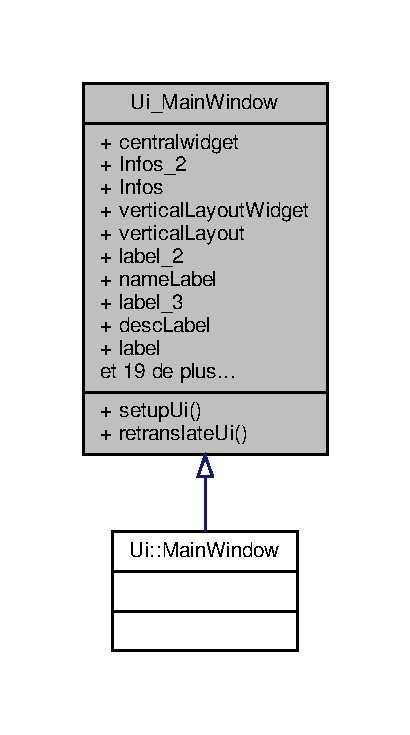
\includegraphics[width=197pt]{classUi__MainWindow__inherit__graph}
\end{center}
\end{figure}


Graphe de collaboration de Ui\+\_\+\+Main\+Window\+:\nopagebreak
\begin{figure}[H]
\begin{center}
\leavevmode
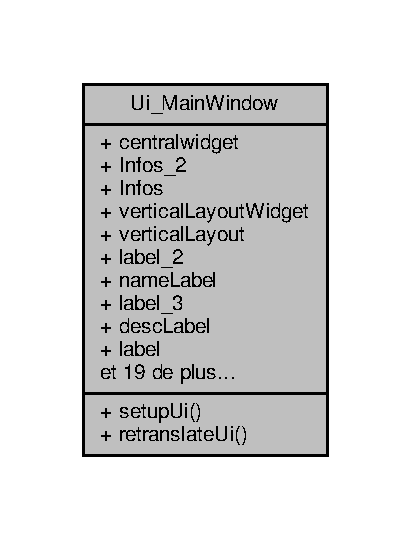
\includegraphics[width=197pt]{classUi__MainWindow__coll__graph}
\end{center}
\end{figure}
\subsection*{Fonctions membres publiques}
\begin{DoxyCompactItemize}
\item 
void \hyperlink{classUi__MainWindow_acf4a0872c4c77d8f43a2ec66ed849b58}{setup\+Ui} (Q\+Main\+Window $\ast$\hyperlink{classMainWindow}{Main\+Window})
\item 
void \hyperlink{classUi__MainWindow_a097dd160c3534a204904cb374412c618}{retranslate\+Ui} (Q\+Main\+Window $\ast$\hyperlink{classMainWindow}{Main\+Window})
\end{DoxyCompactItemize}
\subsection*{Attributs publics}
\begin{DoxyCompactItemize}
\item 
Q\+Widget $\ast$ \hyperlink{classUi__MainWindow_a356f1cf3ebda15f1fac59467ee081b74}{centralwidget}
\item 
Q\+Tab\+Widget $\ast$ \hyperlink{classUi__MainWindow_ad29002426b14e983785a8f2886efbb5d}{Infos\+\_\+2}
\item 
Q\+Widget $\ast$ \hyperlink{classUi__MainWindow_a21abb4cf009e45a4fc597be8e544db3c}{Infos}
\item 
Q\+Widget $\ast$ \hyperlink{classUi__MainWindow_a805d415fff07a22a85219e1f22f2da28}{vertical\+Layout\+Widget}
\item 
Q\+V\+Box\+Layout $\ast$ \hyperlink{classUi__MainWindow_aecd96a04789fcfec3f98d80390ad8184}{vertical\+Layout}
\item 
Q\+Label $\ast$ \hyperlink{classUi__MainWindow_a2e2516d755e4dd53fc905dabddf2738a}{label\+\_\+2}
\item 
Q\+Label $\ast$ \hyperlink{classUi__MainWindow_a134047926bc9eaff33275117ccbc9c21}{name\+Label}
\item 
Q\+Label $\ast$ \hyperlink{classUi__MainWindow_a0376fd90247280e7c7957cc70628708c}{label\+\_\+3}
\item 
Q\+Label $\ast$ \hyperlink{classUi__MainWindow_aef605882ad38f71df7095c44b3bb7a56}{desc\+Label}
\item 
Q\+Label $\ast$ \hyperlink{classUi__MainWindow_ad9c89133780f28e6efa2ec17ceb9cff5}{label}
\item 
Q\+Label $\ast$ \hyperlink{classUi__MainWindow_aeea47f27e4d1c1070f60af267ef06044}{keyword\+Label}
\item 
Q\+Label $\ast$ \hyperlink{classUi__MainWindow_ad6bab8fb8903b8f41afea1218ee52695}{label\+\_\+5}
\item 
Q\+Label $\ast$ \hyperlink{classUi__MainWindow_a1c286339fffe4e58accecda69001e9f5}{time\+Label}
\item 
Q\+Label $\ast$ \hyperlink{classUi__MainWindow_a0946b5474fb7d431e2a4f148f0893d02}{label\+\_\+url}
\item 
Q\+Label $\ast$ \hyperlink{classUi__MainWindow_a2b36727ff7a03214bb218fcffc125854}{image}
\item 
Q\+Widget $\ast$ \hyperlink{classUi__MainWindow_a83495b23cbc6810f81978dc0d584b810}{tab\+\_\+2}
\item 
Q\+Label $\ast$ \hyperlink{classUi__MainWindow_ac149af7acaa4ebc0f835b2d23c65d2c3}{Ing\+Label}
\item 
Q\+Label $\ast$ \hyperlink{classUi__MainWindow_a78c7e10730b43c6700cd7216911ed76a}{label\+\_\+4}
\item 
Q\+Widget $\ast$ \hyperlink{classUi__MainWindow_a3efc28c664e9f5115095aafbbc5ac6bc}{tab}
\item 
Q\+Widget $\ast$ \hyperlink{classUi__MainWindow_acfaf6d66c957965550714c6b9bd0edc0}{vertical\+Layout\+Widget\+\_\+3}
\item 
Q\+V\+Box\+Layout $\ast$ \hyperlink{classUi__MainWindow_a38b8a4b887f3b58e2a49e7905ae6f1f0}{vertical\+Layout\+\_\+3}
\item 
Q\+Label $\ast$ \hyperlink{classUi__MainWindow_aa375f56e2e2ab48391b872c851c21047}{no\+Etapes}
\item 
Q\+Label $\ast$ \hyperlink{classUi__MainWindow_a84aca9c0f7468f334d9865cfadbb543a}{liste\+Etapes}
\item 
Q\+Widget $\ast$ \hyperlink{classUi__MainWindow_a9271976c4376de565bfe96c296f4db1e}{horizontal\+Layout\+Widget}
\item 
Q\+H\+Box\+Layout $\ast$ \hyperlink{classUi__MainWindow_a80867018070156432923d0266cc9fe25}{horizontal\+Layout\+\_\+2}
\item 
Q\+Push\+Button $\ast$ \hyperlink{classUi__MainWindow_ad414d11a8c66c96e45d4d3a6029c4272}{button\+\_\+preced}
\item 
Q\+Push\+Button $\ast$ \hyperlink{classUi__MainWindow_ae5ecde4d9889cfd958321f60285ccdd6}{button\+\_\+suivant}
\item 
Q\+Menu\+Bar $\ast$ \hyperlink{classUi__MainWindow_adf43d9a67adaec750aaa956b5e082f09}{menubar}
\item 
Q\+Status\+Bar $\ast$ \hyperlink{classUi__MainWindow_a1687cceb1e2787aa1f83e50433943a91}{statusbar}
\end{DoxyCompactItemize}


\subsection{Documentation des fonctions membres}
\mbox{\Hypertarget{classUi__MainWindow_a097dd160c3534a204904cb374412c618}\label{classUi__MainWindow_a097dd160c3534a204904cb374412c618}} 
\index{Ui\+\_\+\+Main\+Window@{Ui\+\_\+\+Main\+Window}!retranslate\+Ui@{retranslate\+Ui}}
\index{retranslate\+Ui@{retranslate\+Ui}!Ui\+\_\+\+Main\+Window@{Ui\+\_\+\+Main\+Window}}
\subsubsection{\texorpdfstring{retranslate\+Ui()}{retranslateUi()}}
{\footnotesize\ttfamily void Ui\+\_\+\+Main\+Window\+::retranslate\+Ui (\begin{DoxyParamCaption}\item[{Q\+Main\+Window $\ast$}]{Main\+Window }\end{DoxyParamCaption})\hspace{0.3cm}{\ttfamily [inline]}}

\mbox{\Hypertarget{classUi__MainWindow_acf4a0872c4c77d8f43a2ec66ed849b58}\label{classUi__MainWindow_acf4a0872c4c77d8f43a2ec66ed849b58}} 
\index{Ui\+\_\+\+Main\+Window@{Ui\+\_\+\+Main\+Window}!setup\+Ui@{setup\+Ui}}
\index{setup\+Ui@{setup\+Ui}!Ui\+\_\+\+Main\+Window@{Ui\+\_\+\+Main\+Window}}
\subsubsection{\texorpdfstring{setup\+Ui()}{setupUi()}}
{\footnotesize\ttfamily void Ui\+\_\+\+Main\+Window\+::setup\+Ui (\begin{DoxyParamCaption}\item[{Q\+Main\+Window $\ast$}]{Main\+Window }\end{DoxyParamCaption})\hspace{0.3cm}{\ttfamily [inline]}}



\subsection{Documentation des données membres}
\mbox{\Hypertarget{classUi__MainWindow_ad414d11a8c66c96e45d4d3a6029c4272}\label{classUi__MainWindow_ad414d11a8c66c96e45d4d3a6029c4272}} 
\index{Ui\+\_\+\+Main\+Window@{Ui\+\_\+\+Main\+Window}!button\+\_\+preced@{button\+\_\+preced}}
\index{button\+\_\+preced@{button\+\_\+preced}!Ui\+\_\+\+Main\+Window@{Ui\+\_\+\+Main\+Window}}
\subsubsection{\texorpdfstring{button\+\_\+preced}{button\_preced}}
{\footnotesize\ttfamily Q\+Push\+Button$\ast$ Ui\+\_\+\+Main\+Window\+::button\+\_\+preced}

\mbox{\Hypertarget{classUi__MainWindow_ae5ecde4d9889cfd958321f60285ccdd6}\label{classUi__MainWindow_ae5ecde4d9889cfd958321f60285ccdd6}} 
\index{Ui\+\_\+\+Main\+Window@{Ui\+\_\+\+Main\+Window}!button\+\_\+suivant@{button\+\_\+suivant}}
\index{button\+\_\+suivant@{button\+\_\+suivant}!Ui\+\_\+\+Main\+Window@{Ui\+\_\+\+Main\+Window}}
\subsubsection{\texorpdfstring{button\+\_\+suivant}{button\_suivant}}
{\footnotesize\ttfamily Q\+Push\+Button$\ast$ Ui\+\_\+\+Main\+Window\+::button\+\_\+suivant}

\mbox{\Hypertarget{classUi__MainWindow_a356f1cf3ebda15f1fac59467ee081b74}\label{classUi__MainWindow_a356f1cf3ebda15f1fac59467ee081b74}} 
\index{Ui\+\_\+\+Main\+Window@{Ui\+\_\+\+Main\+Window}!centralwidget@{centralwidget}}
\index{centralwidget@{centralwidget}!Ui\+\_\+\+Main\+Window@{Ui\+\_\+\+Main\+Window}}
\subsubsection{\texorpdfstring{centralwidget}{centralwidget}}
{\footnotesize\ttfamily Q\+Widget$\ast$ Ui\+\_\+\+Main\+Window\+::centralwidget}

\mbox{\Hypertarget{classUi__MainWindow_aef605882ad38f71df7095c44b3bb7a56}\label{classUi__MainWindow_aef605882ad38f71df7095c44b3bb7a56}} 
\index{Ui\+\_\+\+Main\+Window@{Ui\+\_\+\+Main\+Window}!desc\+Label@{desc\+Label}}
\index{desc\+Label@{desc\+Label}!Ui\+\_\+\+Main\+Window@{Ui\+\_\+\+Main\+Window}}
\subsubsection{\texorpdfstring{desc\+Label}{descLabel}}
{\footnotesize\ttfamily Q\+Label$\ast$ Ui\+\_\+\+Main\+Window\+::desc\+Label}

\mbox{\Hypertarget{classUi__MainWindow_a80867018070156432923d0266cc9fe25}\label{classUi__MainWindow_a80867018070156432923d0266cc9fe25}} 
\index{Ui\+\_\+\+Main\+Window@{Ui\+\_\+\+Main\+Window}!horizontal\+Layout\+\_\+2@{horizontal\+Layout\+\_\+2}}
\index{horizontal\+Layout\+\_\+2@{horizontal\+Layout\+\_\+2}!Ui\+\_\+\+Main\+Window@{Ui\+\_\+\+Main\+Window}}
\subsubsection{\texorpdfstring{horizontal\+Layout\+\_\+2}{horizontalLayout\_2}}
{\footnotesize\ttfamily Q\+H\+Box\+Layout$\ast$ Ui\+\_\+\+Main\+Window\+::horizontal\+Layout\+\_\+2}

\mbox{\Hypertarget{classUi__MainWindow_a9271976c4376de565bfe96c296f4db1e}\label{classUi__MainWindow_a9271976c4376de565bfe96c296f4db1e}} 
\index{Ui\+\_\+\+Main\+Window@{Ui\+\_\+\+Main\+Window}!horizontal\+Layout\+Widget@{horizontal\+Layout\+Widget}}
\index{horizontal\+Layout\+Widget@{horizontal\+Layout\+Widget}!Ui\+\_\+\+Main\+Window@{Ui\+\_\+\+Main\+Window}}
\subsubsection{\texorpdfstring{horizontal\+Layout\+Widget}{horizontalLayoutWidget}}
{\footnotesize\ttfamily Q\+Widget$\ast$ Ui\+\_\+\+Main\+Window\+::horizontal\+Layout\+Widget}

\mbox{\Hypertarget{classUi__MainWindow_a2b36727ff7a03214bb218fcffc125854}\label{classUi__MainWindow_a2b36727ff7a03214bb218fcffc125854}} 
\index{Ui\+\_\+\+Main\+Window@{Ui\+\_\+\+Main\+Window}!image@{image}}
\index{image@{image}!Ui\+\_\+\+Main\+Window@{Ui\+\_\+\+Main\+Window}}
\subsubsection{\texorpdfstring{image}{image}}
{\footnotesize\ttfamily Q\+Label$\ast$ Ui\+\_\+\+Main\+Window\+::image}

\mbox{\Hypertarget{classUi__MainWindow_a21abb4cf009e45a4fc597be8e544db3c}\label{classUi__MainWindow_a21abb4cf009e45a4fc597be8e544db3c}} 
\index{Ui\+\_\+\+Main\+Window@{Ui\+\_\+\+Main\+Window}!Infos@{Infos}}
\index{Infos@{Infos}!Ui\+\_\+\+Main\+Window@{Ui\+\_\+\+Main\+Window}}
\subsubsection{\texorpdfstring{Infos}{Infos}}
{\footnotesize\ttfamily Q\+Widget$\ast$ Ui\+\_\+\+Main\+Window\+::\+Infos}

\mbox{\Hypertarget{classUi__MainWindow_ad29002426b14e983785a8f2886efbb5d}\label{classUi__MainWindow_ad29002426b14e983785a8f2886efbb5d}} 
\index{Ui\+\_\+\+Main\+Window@{Ui\+\_\+\+Main\+Window}!Infos\+\_\+2@{Infos\+\_\+2}}
\index{Infos\+\_\+2@{Infos\+\_\+2}!Ui\+\_\+\+Main\+Window@{Ui\+\_\+\+Main\+Window}}
\subsubsection{\texorpdfstring{Infos\+\_\+2}{Infos\_2}}
{\footnotesize\ttfamily Q\+Tab\+Widget$\ast$ Ui\+\_\+\+Main\+Window\+::\+Infos\+\_\+2}

\mbox{\Hypertarget{classUi__MainWindow_ac149af7acaa4ebc0f835b2d23c65d2c3}\label{classUi__MainWindow_ac149af7acaa4ebc0f835b2d23c65d2c3}} 
\index{Ui\+\_\+\+Main\+Window@{Ui\+\_\+\+Main\+Window}!Ing\+Label@{Ing\+Label}}
\index{Ing\+Label@{Ing\+Label}!Ui\+\_\+\+Main\+Window@{Ui\+\_\+\+Main\+Window}}
\subsubsection{\texorpdfstring{Ing\+Label}{IngLabel}}
{\footnotesize\ttfamily Q\+Label$\ast$ Ui\+\_\+\+Main\+Window\+::\+Ing\+Label}

\mbox{\Hypertarget{classUi__MainWindow_aeea47f27e4d1c1070f60af267ef06044}\label{classUi__MainWindow_aeea47f27e4d1c1070f60af267ef06044}} 
\index{Ui\+\_\+\+Main\+Window@{Ui\+\_\+\+Main\+Window}!keyword\+Label@{keyword\+Label}}
\index{keyword\+Label@{keyword\+Label}!Ui\+\_\+\+Main\+Window@{Ui\+\_\+\+Main\+Window}}
\subsubsection{\texorpdfstring{keyword\+Label}{keywordLabel}}
{\footnotesize\ttfamily Q\+Label$\ast$ Ui\+\_\+\+Main\+Window\+::keyword\+Label}

\mbox{\Hypertarget{classUi__MainWindow_ad9c89133780f28e6efa2ec17ceb9cff5}\label{classUi__MainWindow_ad9c89133780f28e6efa2ec17ceb9cff5}} 
\index{Ui\+\_\+\+Main\+Window@{Ui\+\_\+\+Main\+Window}!label@{label}}
\index{label@{label}!Ui\+\_\+\+Main\+Window@{Ui\+\_\+\+Main\+Window}}
\subsubsection{\texorpdfstring{label}{label}}
{\footnotesize\ttfamily Q\+Label$\ast$ Ui\+\_\+\+Main\+Window\+::label}

\mbox{\Hypertarget{classUi__MainWindow_a2e2516d755e4dd53fc905dabddf2738a}\label{classUi__MainWindow_a2e2516d755e4dd53fc905dabddf2738a}} 
\index{Ui\+\_\+\+Main\+Window@{Ui\+\_\+\+Main\+Window}!label\+\_\+2@{label\+\_\+2}}
\index{label\+\_\+2@{label\+\_\+2}!Ui\+\_\+\+Main\+Window@{Ui\+\_\+\+Main\+Window}}
\subsubsection{\texorpdfstring{label\+\_\+2}{label\_2}}
{\footnotesize\ttfamily Q\+Label$\ast$ Ui\+\_\+\+Main\+Window\+::label\+\_\+2}

\mbox{\Hypertarget{classUi__MainWindow_a0376fd90247280e7c7957cc70628708c}\label{classUi__MainWindow_a0376fd90247280e7c7957cc70628708c}} 
\index{Ui\+\_\+\+Main\+Window@{Ui\+\_\+\+Main\+Window}!label\+\_\+3@{label\+\_\+3}}
\index{label\+\_\+3@{label\+\_\+3}!Ui\+\_\+\+Main\+Window@{Ui\+\_\+\+Main\+Window}}
\subsubsection{\texorpdfstring{label\+\_\+3}{label\_3}}
{\footnotesize\ttfamily Q\+Label$\ast$ Ui\+\_\+\+Main\+Window\+::label\+\_\+3}

\mbox{\Hypertarget{classUi__MainWindow_a78c7e10730b43c6700cd7216911ed76a}\label{classUi__MainWindow_a78c7e10730b43c6700cd7216911ed76a}} 
\index{Ui\+\_\+\+Main\+Window@{Ui\+\_\+\+Main\+Window}!label\+\_\+4@{label\+\_\+4}}
\index{label\+\_\+4@{label\+\_\+4}!Ui\+\_\+\+Main\+Window@{Ui\+\_\+\+Main\+Window}}
\subsubsection{\texorpdfstring{label\+\_\+4}{label\_4}}
{\footnotesize\ttfamily Q\+Label$\ast$ Ui\+\_\+\+Main\+Window\+::label\+\_\+4}

\mbox{\Hypertarget{classUi__MainWindow_ad6bab8fb8903b8f41afea1218ee52695}\label{classUi__MainWindow_ad6bab8fb8903b8f41afea1218ee52695}} 
\index{Ui\+\_\+\+Main\+Window@{Ui\+\_\+\+Main\+Window}!label\+\_\+5@{label\+\_\+5}}
\index{label\+\_\+5@{label\+\_\+5}!Ui\+\_\+\+Main\+Window@{Ui\+\_\+\+Main\+Window}}
\subsubsection{\texorpdfstring{label\+\_\+5}{label\_5}}
{\footnotesize\ttfamily Q\+Label$\ast$ Ui\+\_\+\+Main\+Window\+::label\+\_\+5}

\mbox{\Hypertarget{classUi__MainWindow_a0946b5474fb7d431e2a4f148f0893d02}\label{classUi__MainWindow_a0946b5474fb7d431e2a4f148f0893d02}} 
\index{Ui\+\_\+\+Main\+Window@{Ui\+\_\+\+Main\+Window}!label\+\_\+url@{label\+\_\+url}}
\index{label\+\_\+url@{label\+\_\+url}!Ui\+\_\+\+Main\+Window@{Ui\+\_\+\+Main\+Window}}
\subsubsection{\texorpdfstring{label\+\_\+url}{label\_url}}
{\footnotesize\ttfamily Q\+Label$\ast$ Ui\+\_\+\+Main\+Window\+::label\+\_\+url}

\mbox{\Hypertarget{classUi__MainWindow_a84aca9c0f7468f334d9865cfadbb543a}\label{classUi__MainWindow_a84aca9c0f7468f334d9865cfadbb543a}} 
\index{Ui\+\_\+\+Main\+Window@{Ui\+\_\+\+Main\+Window}!liste\+Etapes@{liste\+Etapes}}
\index{liste\+Etapes@{liste\+Etapes}!Ui\+\_\+\+Main\+Window@{Ui\+\_\+\+Main\+Window}}
\subsubsection{\texorpdfstring{liste\+Etapes}{listeEtapes}}
{\footnotesize\ttfamily Q\+Label$\ast$ Ui\+\_\+\+Main\+Window\+::liste\+Etapes}

\mbox{\Hypertarget{classUi__MainWindow_adf43d9a67adaec750aaa956b5e082f09}\label{classUi__MainWindow_adf43d9a67adaec750aaa956b5e082f09}} 
\index{Ui\+\_\+\+Main\+Window@{Ui\+\_\+\+Main\+Window}!menubar@{menubar}}
\index{menubar@{menubar}!Ui\+\_\+\+Main\+Window@{Ui\+\_\+\+Main\+Window}}
\subsubsection{\texorpdfstring{menubar}{menubar}}
{\footnotesize\ttfamily Q\+Menu\+Bar$\ast$ Ui\+\_\+\+Main\+Window\+::menubar}

\mbox{\Hypertarget{classUi__MainWindow_a134047926bc9eaff33275117ccbc9c21}\label{classUi__MainWindow_a134047926bc9eaff33275117ccbc9c21}} 
\index{Ui\+\_\+\+Main\+Window@{Ui\+\_\+\+Main\+Window}!name\+Label@{name\+Label}}
\index{name\+Label@{name\+Label}!Ui\+\_\+\+Main\+Window@{Ui\+\_\+\+Main\+Window}}
\subsubsection{\texorpdfstring{name\+Label}{nameLabel}}
{\footnotesize\ttfamily Q\+Label$\ast$ Ui\+\_\+\+Main\+Window\+::name\+Label}

\mbox{\Hypertarget{classUi__MainWindow_aa375f56e2e2ab48391b872c851c21047}\label{classUi__MainWindow_aa375f56e2e2ab48391b872c851c21047}} 
\index{Ui\+\_\+\+Main\+Window@{Ui\+\_\+\+Main\+Window}!no\+Etapes@{no\+Etapes}}
\index{no\+Etapes@{no\+Etapes}!Ui\+\_\+\+Main\+Window@{Ui\+\_\+\+Main\+Window}}
\subsubsection{\texorpdfstring{no\+Etapes}{noEtapes}}
{\footnotesize\ttfamily Q\+Label$\ast$ Ui\+\_\+\+Main\+Window\+::no\+Etapes}

\mbox{\Hypertarget{classUi__MainWindow_a1687cceb1e2787aa1f83e50433943a91}\label{classUi__MainWindow_a1687cceb1e2787aa1f83e50433943a91}} 
\index{Ui\+\_\+\+Main\+Window@{Ui\+\_\+\+Main\+Window}!statusbar@{statusbar}}
\index{statusbar@{statusbar}!Ui\+\_\+\+Main\+Window@{Ui\+\_\+\+Main\+Window}}
\subsubsection{\texorpdfstring{statusbar}{statusbar}}
{\footnotesize\ttfamily Q\+Status\+Bar$\ast$ Ui\+\_\+\+Main\+Window\+::statusbar}

\mbox{\Hypertarget{classUi__MainWindow_a3efc28c664e9f5115095aafbbc5ac6bc}\label{classUi__MainWindow_a3efc28c664e9f5115095aafbbc5ac6bc}} 
\index{Ui\+\_\+\+Main\+Window@{Ui\+\_\+\+Main\+Window}!tab@{tab}}
\index{tab@{tab}!Ui\+\_\+\+Main\+Window@{Ui\+\_\+\+Main\+Window}}
\subsubsection{\texorpdfstring{tab}{tab}}
{\footnotesize\ttfamily Q\+Widget$\ast$ Ui\+\_\+\+Main\+Window\+::tab}

\mbox{\Hypertarget{classUi__MainWindow_a83495b23cbc6810f81978dc0d584b810}\label{classUi__MainWindow_a83495b23cbc6810f81978dc0d584b810}} 
\index{Ui\+\_\+\+Main\+Window@{Ui\+\_\+\+Main\+Window}!tab\+\_\+2@{tab\+\_\+2}}
\index{tab\+\_\+2@{tab\+\_\+2}!Ui\+\_\+\+Main\+Window@{Ui\+\_\+\+Main\+Window}}
\subsubsection{\texorpdfstring{tab\+\_\+2}{tab\_2}}
{\footnotesize\ttfamily Q\+Widget$\ast$ Ui\+\_\+\+Main\+Window\+::tab\+\_\+2}

\mbox{\Hypertarget{classUi__MainWindow_a1c286339fffe4e58accecda69001e9f5}\label{classUi__MainWindow_a1c286339fffe4e58accecda69001e9f5}} 
\index{Ui\+\_\+\+Main\+Window@{Ui\+\_\+\+Main\+Window}!time\+Label@{time\+Label}}
\index{time\+Label@{time\+Label}!Ui\+\_\+\+Main\+Window@{Ui\+\_\+\+Main\+Window}}
\subsubsection{\texorpdfstring{time\+Label}{timeLabel}}
{\footnotesize\ttfamily Q\+Label$\ast$ Ui\+\_\+\+Main\+Window\+::time\+Label}

\mbox{\Hypertarget{classUi__MainWindow_aecd96a04789fcfec3f98d80390ad8184}\label{classUi__MainWindow_aecd96a04789fcfec3f98d80390ad8184}} 
\index{Ui\+\_\+\+Main\+Window@{Ui\+\_\+\+Main\+Window}!vertical\+Layout@{vertical\+Layout}}
\index{vertical\+Layout@{vertical\+Layout}!Ui\+\_\+\+Main\+Window@{Ui\+\_\+\+Main\+Window}}
\subsubsection{\texorpdfstring{vertical\+Layout}{verticalLayout}}
{\footnotesize\ttfamily Q\+V\+Box\+Layout$\ast$ Ui\+\_\+\+Main\+Window\+::vertical\+Layout}

\mbox{\Hypertarget{classUi__MainWindow_a38b8a4b887f3b58e2a49e7905ae6f1f0}\label{classUi__MainWindow_a38b8a4b887f3b58e2a49e7905ae6f1f0}} 
\index{Ui\+\_\+\+Main\+Window@{Ui\+\_\+\+Main\+Window}!vertical\+Layout\+\_\+3@{vertical\+Layout\+\_\+3}}
\index{vertical\+Layout\+\_\+3@{vertical\+Layout\+\_\+3}!Ui\+\_\+\+Main\+Window@{Ui\+\_\+\+Main\+Window}}
\subsubsection{\texorpdfstring{vertical\+Layout\+\_\+3}{verticalLayout\_3}}
{\footnotesize\ttfamily Q\+V\+Box\+Layout$\ast$ Ui\+\_\+\+Main\+Window\+::vertical\+Layout\+\_\+3}

\mbox{\Hypertarget{classUi__MainWindow_a805d415fff07a22a85219e1f22f2da28}\label{classUi__MainWindow_a805d415fff07a22a85219e1f22f2da28}} 
\index{Ui\+\_\+\+Main\+Window@{Ui\+\_\+\+Main\+Window}!vertical\+Layout\+Widget@{vertical\+Layout\+Widget}}
\index{vertical\+Layout\+Widget@{vertical\+Layout\+Widget}!Ui\+\_\+\+Main\+Window@{Ui\+\_\+\+Main\+Window}}
\subsubsection{\texorpdfstring{vertical\+Layout\+Widget}{verticalLayoutWidget}}
{\footnotesize\ttfamily Q\+Widget$\ast$ Ui\+\_\+\+Main\+Window\+::vertical\+Layout\+Widget}

\mbox{\Hypertarget{classUi__MainWindow_acfaf6d66c957965550714c6b9bd0edc0}\label{classUi__MainWindow_acfaf6d66c957965550714c6b9bd0edc0}} 
\index{Ui\+\_\+\+Main\+Window@{Ui\+\_\+\+Main\+Window}!vertical\+Layout\+Widget\+\_\+3@{vertical\+Layout\+Widget\+\_\+3}}
\index{vertical\+Layout\+Widget\+\_\+3@{vertical\+Layout\+Widget\+\_\+3}!Ui\+\_\+\+Main\+Window@{Ui\+\_\+\+Main\+Window}}
\subsubsection{\texorpdfstring{vertical\+Layout\+Widget\+\_\+3}{verticalLayoutWidget\_3}}
{\footnotesize\ttfamily Q\+Widget$\ast$ Ui\+\_\+\+Main\+Window\+::vertical\+Layout\+Widget\+\_\+3}



La documentation de cette classe a été générée à partir du fichier suivant \+:\begin{DoxyCompactItemize}
\item 
\hyperlink{ui__mainwindow_8h}{ui\+\_\+mainwindow.\+h}\end{DoxyCompactItemize}

\hypertarget{classUi__MainWindowLaunchDialog}{}\section{Référence de la classe Ui\+\_\+\+Main\+Window\+Launch\+Dialog}
\label{classUi__MainWindowLaunchDialog}\index{Ui\+\_\+\+Main\+Window\+Launch\+Dialog@{Ui\+\_\+\+Main\+Window\+Launch\+Dialog}}


{\ttfamily \#include $<$ui\+\_\+mainwindowlaunchdialog.\+h$>$}



Graphe d\textquotesingle{}héritage de Ui\+\_\+\+Main\+Window\+Launch\+Dialog\+:\nopagebreak
\begin{figure}[H]
\begin{center}
\leavevmode
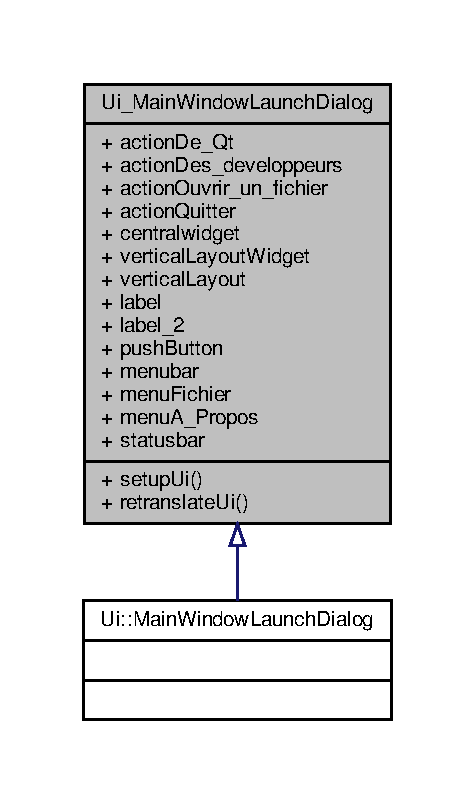
\includegraphics[width=228pt]{classUi__MainWindowLaunchDialog__inherit__graph}
\end{center}
\end{figure}


Graphe de collaboration de Ui\+\_\+\+Main\+Window\+Launch\+Dialog\+:\nopagebreak
\begin{figure}[H]
\begin{center}
\leavevmode
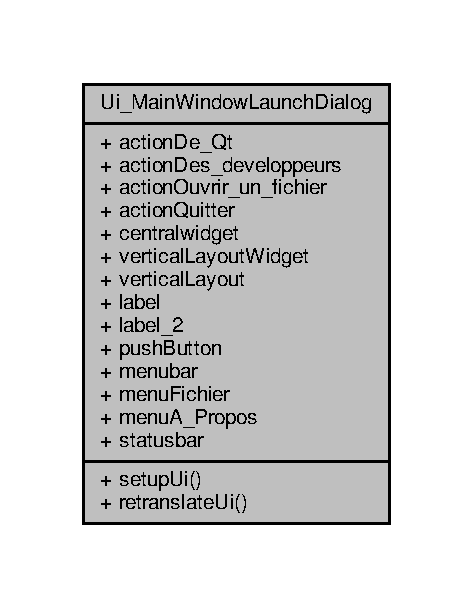
\includegraphics[width=227pt]{classUi__MainWindowLaunchDialog__coll__graph}
\end{center}
\end{figure}
\subsection*{Fonctions membres publiques}
\begin{DoxyCompactItemize}
\item 
void \hyperlink{classUi__MainWindowLaunchDialog_aaf6508e53a3297d30c982c8f49b9ad61}{setup\+Ui} (Q\+Main\+Window $\ast$\hyperlink{classMainWindowLaunchDialog}{Main\+Window\+Launch\+Dialog})
\item 
void \hyperlink{classUi__MainWindowLaunchDialog_ab0d2fbf998b405c114cd669a247a10fa}{retranslate\+Ui} (Q\+Main\+Window $\ast$\hyperlink{classMainWindowLaunchDialog}{Main\+Window\+Launch\+Dialog})
\end{DoxyCompactItemize}
\subsection*{Attributs publics}
\begin{DoxyCompactItemize}
\item 
Q\+Action $\ast$ \hyperlink{classUi__MainWindowLaunchDialog_ad330b743b240886eec788d726229510c}{action\+De\+\_\+\+Qt}
\item 
Q\+Action $\ast$ \hyperlink{classUi__MainWindowLaunchDialog_ad35fac29b9df90655a3afcfda6f593d7}{action\+Des\+\_\+developpeurs}
\item 
Q\+Action $\ast$ \hyperlink{classUi__MainWindowLaunchDialog_a1f2289cb780a2b574328bb9eeb72d2ae}{action\+Ouvrir\+\_\+un\+\_\+fichier}
\item 
Q\+Action $\ast$ \hyperlink{classUi__MainWindowLaunchDialog_a79e4a5fecf0b677f688db0d27fd85883}{action\+Quitter}
\item 
Q\+Widget $\ast$ \hyperlink{classUi__MainWindowLaunchDialog_aa830f03176134817a5d0f829f80b98c7}{centralwidget}
\item 
Q\+Widget $\ast$ \hyperlink{classUi__MainWindowLaunchDialog_a18052818965cf103bed3e6dbbf72fac8}{vertical\+Layout\+Widget}
\item 
Q\+V\+Box\+Layout $\ast$ \hyperlink{classUi__MainWindowLaunchDialog_a249a932d8ac5a63462b4e5ee0084b959}{vertical\+Layout}
\item 
Q\+Label $\ast$ \hyperlink{classUi__MainWindowLaunchDialog_a74a25c82a489e8e5b2c02230e66702cf}{label}
\item 
Q\+Label $\ast$ \hyperlink{classUi__MainWindowLaunchDialog_a5365f56fbc86828b5ffe9354c0155d88}{label\+\_\+2}
\item 
Q\+Push\+Button $\ast$ \hyperlink{classUi__MainWindowLaunchDialog_a1f7427c8637b108ce3dd4e5c237ed91c}{push\+Button}
\item 
Q\+Menu\+Bar $\ast$ \hyperlink{classUi__MainWindowLaunchDialog_abe91ed6036fff89837665caa8d52881e}{menubar}
\item 
Q\+Menu $\ast$ \hyperlink{classUi__MainWindowLaunchDialog_ac84cdb6c1fd07e050bcd9f27c6fa7487}{menu\+Fichier}
\item 
Q\+Menu $\ast$ \hyperlink{classUi__MainWindowLaunchDialog_a07a3daedceb3e705eeaef8fb62fe0c38}{menu\+A\+\_\+\+Propos}
\item 
Q\+Status\+Bar $\ast$ \hyperlink{classUi__MainWindowLaunchDialog_ae5d4599a0e0a01dccb6ec5212639d73d}{statusbar}
\end{DoxyCompactItemize}


\subsection{Documentation des fonctions membres}
\mbox{\Hypertarget{classUi__MainWindowLaunchDialog_ab0d2fbf998b405c114cd669a247a10fa}\label{classUi__MainWindowLaunchDialog_ab0d2fbf998b405c114cd669a247a10fa}} 
\index{Ui\+\_\+\+Main\+Window\+Launch\+Dialog@{Ui\+\_\+\+Main\+Window\+Launch\+Dialog}!retranslate\+Ui@{retranslate\+Ui}}
\index{retranslate\+Ui@{retranslate\+Ui}!Ui\+\_\+\+Main\+Window\+Launch\+Dialog@{Ui\+\_\+\+Main\+Window\+Launch\+Dialog}}
\subsubsection{\texorpdfstring{retranslate\+Ui()}{retranslateUi()}}
{\footnotesize\ttfamily void Ui\+\_\+\+Main\+Window\+Launch\+Dialog\+::retranslate\+Ui (\begin{DoxyParamCaption}\item[{Q\+Main\+Window $\ast$}]{Main\+Window\+Launch\+Dialog }\end{DoxyParamCaption})\hspace{0.3cm}{\ttfamily [inline]}}

\mbox{\Hypertarget{classUi__MainWindowLaunchDialog_aaf6508e53a3297d30c982c8f49b9ad61}\label{classUi__MainWindowLaunchDialog_aaf6508e53a3297d30c982c8f49b9ad61}} 
\index{Ui\+\_\+\+Main\+Window\+Launch\+Dialog@{Ui\+\_\+\+Main\+Window\+Launch\+Dialog}!setup\+Ui@{setup\+Ui}}
\index{setup\+Ui@{setup\+Ui}!Ui\+\_\+\+Main\+Window\+Launch\+Dialog@{Ui\+\_\+\+Main\+Window\+Launch\+Dialog}}
\subsubsection{\texorpdfstring{setup\+Ui()}{setupUi()}}
{\footnotesize\ttfamily void Ui\+\_\+\+Main\+Window\+Launch\+Dialog\+::setup\+Ui (\begin{DoxyParamCaption}\item[{Q\+Main\+Window $\ast$}]{Main\+Window\+Launch\+Dialog }\end{DoxyParamCaption})\hspace{0.3cm}{\ttfamily [inline]}}



\subsection{Documentation des données membres}
\mbox{\Hypertarget{classUi__MainWindowLaunchDialog_ad330b743b240886eec788d726229510c}\label{classUi__MainWindowLaunchDialog_ad330b743b240886eec788d726229510c}} 
\index{Ui\+\_\+\+Main\+Window\+Launch\+Dialog@{Ui\+\_\+\+Main\+Window\+Launch\+Dialog}!action\+De\+\_\+\+Qt@{action\+De\+\_\+\+Qt}}
\index{action\+De\+\_\+\+Qt@{action\+De\+\_\+\+Qt}!Ui\+\_\+\+Main\+Window\+Launch\+Dialog@{Ui\+\_\+\+Main\+Window\+Launch\+Dialog}}
\subsubsection{\texorpdfstring{action\+De\+\_\+\+Qt}{actionDe\_Qt}}
{\footnotesize\ttfamily Q\+Action$\ast$ Ui\+\_\+\+Main\+Window\+Launch\+Dialog\+::action\+De\+\_\+\+Qt}

\mbox{\Hypertarget{classUi__MainWindowLaunchDialog_ad35fac29b9df90655a3afcfda6f593d7}\label{classUi__MainWindowLaunchDialog_ad35fac29b9df90655a3afcfda6f593d7}} 
\index{Ui\+\_\+\+Main\+Window\+Launch\+Dialog@{Ui\+\_\+\+Main\+Window\+Launch\+Dialog}!action\+Des\+\_\+developpeurs@{action\+Des\+\_\+developpeurs}}
\index{action\+Des\+\_\+developpeurs@{action\+Des\+\_\+developpeurs}!Ui\+\_\+\+Main\+Window\+Launch\+Dialog@{Ui\+\_\+\+Main\+Window\+Launch\+Dialog}}
\subsubsection{\texorpdfstring{action\+Des\+\_\+developpeurs}{actionDes\_developpeurs}}
{\footnotesize\ttfamily Q\+Action$\ast$ Ui\+\_\+\+Main\+Window\+Launch\+Dialog\+::action\+Des\+\_\+developpeurs}

\mbox{\Hypertarget{classUi__MainWindowLaunchDialog_a1f2289cb780a2b574328bb9eeb72d2ae}\label{classUi__MainWindowLaunchDialog_a1f2289cb780a2b574328bb9eeb72d2ae}} 
\index{Ui\+\_\+\+Main\+Window\+Launch\+Dialog@{Ui\+\_\+\+Main\+Window\+Launch\+Dialog}!action\+Ouvrir\+\_\+un\+\_\+fichier@{action\+Ouvrir\+\_\+un\+\_\+fichier}}
\index{action\+Ouvrir\+\_\+un\+\_\+fichier@{action\+Ouvrir\+\_\+un\+\_\+fichier}!Ui\+\_\+\+Main\+Window\+Launch\+Dialog@{Ui\+\_\+\+Main\+Window\+Launch\+Dialog}}
\subsubsection{\texorpdfstring{action\+Ouvrir\+\_\+un\+\_\+fichier}{actionOuvrir\_un\_fichier}}
{\footnotesize\ttfamily Q\+Action$\ast$ Ui\+\_\+\+Main\+Window\+Launch\+Dialog\+::action\+Ouvrir\+\_\+un\+\_\+fichier}

\mbox{\Hypertarget{classUi__MainWindowLaunchDialog_a79e4a5fecf0b677f688db0d27fd85883}\label{classUi__MainWindowLaunchDialog_a79e4a5fecf0b677f688db0d27fd85883}} 
\index{Ui\+\_\+\+Main\+Window\+Launch\+Dialog@{Ui\+\_\+\+Main\+Window\+Launch\+Dialog}!action\+Quitter@{action\+Quitter}}
\index{action\+Quitter@{action\+Quitter}!Ui\+\_\+\+Main\+Window\+Launch\+Dialog@{Ui\+\_\+\+Main\+Window\+Launch\+Dialog}}
\subsubsection{\texorpdfstring{action\+Quitter}{actionQuitter}}
{\footnotesize\ttfamily Q\+Action$\ast$ Ui\+\_\+\+Main\+Window\+Launch\+Dialog\+::action\+Quitter}

\mbox{\Hypertarget{classUi__MainWindowLaunchDialog_aa830f03176134817a5d0f829f80b98c7}\label{classUi__MainWindowLaunchDialog_aa830f03176134817a5d0f829f80b98c7}} 
\index{Ui\+\_\+\+Main\+Window\+Launch\+Dialog@{Ui\+\_\+\+Main\+Window\+Launch\+Dialog}!centralwidget@{centralwidget}}
\index{centralwidget@{centralwidget}!Ui\+\_\+\+Main\+Window\+Launch\+Dialog@{Ui\+\_\+\+Main\+Window\+Launch\+Dialog}}
\subsubsection{\texorpdfstring{centralwidget}{centralwidget}}
{\footnotesize\ttfamily Q\+Widget$\ast$ Ui\+\_\+\+Main\+Window\+Launch\+Dialog\+::centralwidget}

\mbox{\Hypertarget{classUi__MainWindowLaunchDialog_a74a25c82a489e8e5b2c02230e66702cf}\label{classUi__MainWindowLaunchDialog_a74a25c82a489e8e5b2c02230e66702cf}} 
\index{Ui\+\_\+\+Main\+Window\+Launch\+Dialog@{Ui\+\_\+\+Main\+Window\+Launch\+Dialog}!label@{label}}
\index{label@{label}!Ui\+\_\+\+Main\+Window\+Launch\+Dialog@{Ui\+\_\+\+Main\+Window\+Launch\+Dialog}}
\subsubsection{\texorpdfstring{label}{label}}
{\footnotesize\ttfamily Q\+Label$\ast$ Ui\+\_\+\+Main\+Window\+Launch\+Dialog\+::label}

\mbox{\Hypertarget{classUi__MainWindowLaunchDialog_a5365f56fbc86828b5ffe9354c0155d88}\label{classUi__MainWindowLaunchDialog_a5365f56fbc86828b5ffe9354c0155d88}} 
\index{Ui\+\_\+\+Main\+Window\+Launch\+Dialog@{Ui\+\_\+\+Main\+Window\+Launch\+Dialog}!label\+\_\+2@{label\+\_\+2}}
\index{label\+\_\+2@{label\+\_\+2}!Ui\+\_\+\+Main\+Window\+Launch\+Dialog@{Ui\+\_\+\+Main\+Window\+Launch\+Dialog}}
\subsubsection{\texorpdfstring{label\+\_\+2}{label\_2}}
{\footnotesize\ttfamily Q\+Label$\ast$ Ui\+\_\+\+Main\+Window\+Launch\+Dialog\+::label\+\_\+2}

\mbox{\Hypertarget{classUi__MainWindowLaunchDialog_a07a3daedceb3e705eeaef8fb62fe0c38}\label{classUi__MainWindowLaunchDialog_a07a3daedceb3e705eeaef8fb62fe0c38}} 
\index{Ui\+\_\+\+Main\+Window\+Launch\+Dialog@{Ui\+\_\+\+Main\+Window\+Launch\+Dialog}!menu\+A\+\_\+\+Propos@{menu\+A\+\_\+\+Propos}}
\index{menu\+A\+\_\+\+Propos@{menu\+A\+\_\+\+Propos}!Ui\+\_\+\+Main\+Window\+Launch\+Dialog@{Ui\+\_\+\+Main\+Window\+Launch\+Dialog}}
\subsubsection{\texorpdfstring{menu\+A\+\_\+\+Propos}{menuA\_Propos}}
{\footnotesize\ttfamily Q\+Menu$\ast$ Ui\+\_\+\+Main\+Window\+Launch\+Dialog\+::menu\+A\+\_\+\+Propos}

\mbox{\Hypertarget{classUi__MainWindowLaunchDialog_abe91ed6036fff89837665caa8d52881e}\label{classUi__MainWindowLaunchDialog_abe91ed6036fff89837665caa8d52881e}} 
\index{Ui\+\_\+\+Main\+Window\+Launch\+Dialog@{Ui\+\_\+\+Main\+Window\+Launch\+Dialog}!menubar@{menubar}}
\index{menubar@{menubar}!Ui\+\_\+\+Main\+Window\+Launch\+Dialog@{Ui\+\_\+\+Main\+Window\+Launch\+Dialog}}
\subsubsection{\texorpdfstring{menubar}{menubar}}
{\footnotesize\ttfamily Q\+Menu\+Bar$\ast$ Ui\+\_\+\+Main\+Window\+Launch\+Dialog\+::menubar}

\mbox{\Hypertarget{classUi__MainWindowLaunchDialog_ac84cdb6c1fd07e050bcd9f27c6fa7487}\label{classUi__MainWindowLaunchDialog_ac84cdb6c1fd07e050bcd9f27c6fa7487}} 
\index{Ui\+\_\+\+Main\+Window\+Launch\+Dialog@{Ui\+\_\+\+Main\+Window\+Launch\+Dialog}!menu\+Fichier@{menu\+Fichier}}
\index{menu\+Fichier@{menu\+Fichier}!Ui\+\_\+\+Main\+Window\+Launch\+Dialog@{Ui\+\_\+\+Main\+Window\+Launch\+Dialog}}
\subsubsection{\texorpdfstring{menu\+Fichier}{menuFichier}}
{\footnotesize\ttfamily Q\+Menu$\ast$ Ui\+\_\+\+Main\+Window\+Launch\+Dialog\+::menu\+Fichier}

\mbox{\Hypertarget{classUi__MainWindowLaunchDialog_a1f7427c8637b108ce3dd4e5c237ed91c}\label{classUi__MainWindowLaunchDialog_a1f7427c8637b108ce3dd4e5c237ed91c}} 
\index{Ui\+\_\+\+Main\+Window\+Launch\+Dialog@{Ui\+\_\+\+Main\+Window\+Launch\+Dialog}!push\+Button@{push\+Button}}
\index{push\+Button@{push\+Button}!Ui\+\_\+\+Main\+Window\+Launch\+Dialog@{Ui\+\_\+\+Main\+Window\+Launch\+Dialog}}
\subsubsection{\texorpdfstring{push\+Button}{pushButton}}
{\footnotesize\ttfamily Q\+Push\+Button$\ast$ Ui\+\_\+\+Main\+Window\+Launch\+Dialog\+::push\+Button}

\mbox{\Hypertarget{classUi__MainWindowLaunchDialog_ae5d4599a0e0a01dccb6ec5212639d73d}\label{classUi__MainWindowLaunchDialog_ae5d4599a0e0a01dccb6ec5212639d73d}} 
\index{Ui\+\_\+\+Main\+Window\+Launch\+Dialog@{Ui\+\_\+\+Main\+Window\+Launch\+Dialog}!statusbar@{statusbar}}
\index{statusbar@{statusbar}!Ui\+\_\+\+Main\+Window\+Launch\+Dialog@{Ui\+\_\+\+Main\+Window\+Launch\+Dialog}}
\subsubsection{\texorpdfstring{statusbar}{statusbar}}
{\footnotesize\ttfamily Q\+Status\+Bar$\ast$ Ui\+\_\+\+Main\+Window\+Launch\+Dialog\+::statusbar}

\mbox{\Hypertarget{classUi__MainWindowLaunchDialog_a249a932d8ac5a63462b4e5ee0084b959}\label{classUi__MainWindowLaunchDialog_a249a932d8ac5a63462b4e5ee0084b959}} 
\index{Ui\+\_\+\+Main\+Window\+Launch\+Dialog@{Ui\+\_\+\+Main\+Window\+Launch\+Dialog}!vertical\+Layout@{vertical\+Layout}}
\index{vertical\+Layout@{vertical\+Layout}!Ui\+\_\+\+Main\+Window\+Launch\+Dialog@{Ui\+\_\+\+Main\+Window\+Launch\+Dialog}}
\subsubsection{\texorpdfstring{vertical\+Layout}{verticalLayout}}
{\footnotesize\ttfamily Q\+V\+Box\+Layout$\ast$ Ui\+\_\+\+Main\+Window\+Launch\+Dialog\+::vertical\+Layout}

\mbox{\Hypertarget{classUi__MainWindowLaunchDialog_a18052818965cf103bed3e6dbbf72fac8}\label{classUi__MainWindowLaunchDialog_a18052818965cf103bed3e6dbbf72fac8}} 
\index{Ui\+\_\+\+Main\+Window\+Launch\+Dialog@{Ui\+\_\+\+Main\+Window\+Launch\+Dialog}!vertical\+Layout\+Widget@{vertical\+Layout\+Widget}}
\index{vertical\+Layout\+Widget@{vertical\+Layout\+Widget}!Ui\+\_\+\+Main\+Window\+Launch\+Dialog@{Ui\+\_\+\+Main\+Window\+Launch\+Dialog}}
\subsubsection{\texorpdfstring{vertical\+Layout\+Widget}{verticalLayoutWidget}}
{\footnotesize\ttfamily Q\+Widget$\ast$ Ui\+\_\+\+Main\+Window\+Launch\+Dialog\+::vertical\+Layout\+Widget}



La documentation de cette classe a été générée à partir du fichier suivant \+:\begin{DoxyCompactItemize}
\item 
\hyperlink{ui__mainwindowlaunchdialog_8h}{ui\+\_\+mainwindowlaunchdialog.\+h}\end{DoxyCompactItemize}

\chapter{Documentation des fichiers}
\hypertarget{lecture__json_8cpp}{}\section{lecture\+\_\+json.\+cpp File Reference}
\label{lecture__json_8cpp}\index{lecture\+\_\+json.\+cpp@{lecture\+\_\+json.\+cpp}}


Classe gérant la lecture du fichier json.  


{\ttfamily \#include \char`\"{}lecture\+\_\+json.\+h\char`\"{}}\newline
{\ttfamily \#include \char`\"{}mainwindow.\+h\char`\"{}}\newline
{\ttfamily \#include \char`\"{}traitement.\+h\char`\"{}}\newline
{\ttfamily \#include $<$Q\+File$>$}\newline
{\ttfamily \#include $<$Q\+Json\+Document$>$}\newline
{\ttfamily \#include $<$Q\+Debug$>$}\newline
{\ttfamily \#include $<$Q\+Json\+Object$>$}\newline
{\ttfamily \#include $<$Q\+Json\+Array$>$}\newline
{\ttfamily \#include $<$Q\+Object$>$}\newline
Include dependency graph for lecture\+\_\+json.\+cpp\+:\nopagebreak
\begin{figure}[H]
\begin{center}
\leavevmode
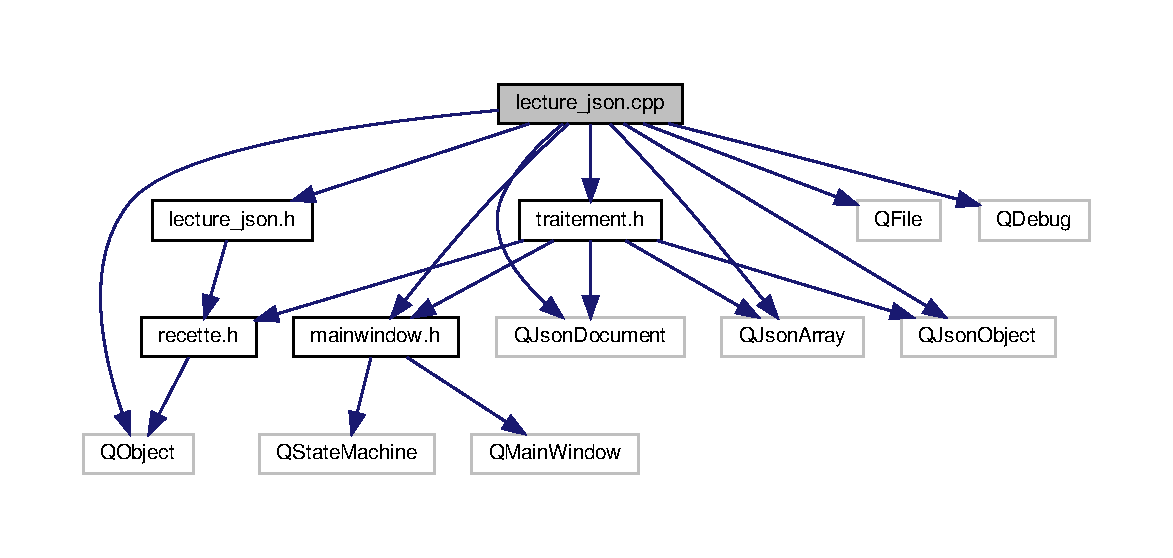
\includegraphics[width=350pt]{lecture__json_8cpp__incl}
\end{center}
\end{figure}


\subsection{Detailed Description}
Classe gérant la lecture du fichier json. 

\begin{DoxyAuthor}{Author}
Pollet Lucas -\/ Fougerouse Arsène 
\end{DoxyAuthor}

\hypertarget{lecture__json_8h}{}\doxysection{lecture\+\_\+json.\+h File Reference}
\label{lecture__json_8h}\index{lecture\_json.h@{lecture\_json.h}}


Classe gérant la lecture du fichier json.  


{\ttfamily \#include \char`\"{}recette.\+h\char`\"{}}\newline
Include dependency graph for lecture\+\_\+json.\+h\+:\nopagebreak
\begin{figure}[H]
\begin{center}
\leavevmode
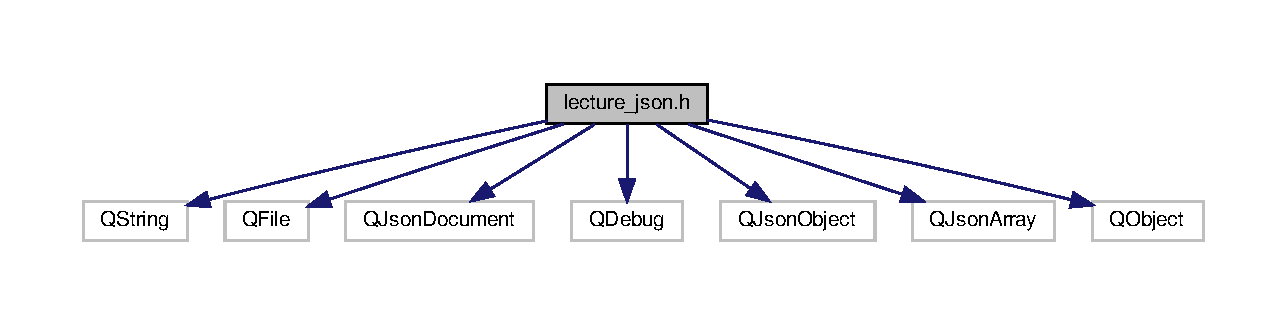
\includegraphics[width=165pt]{lecture__json_8h__incl}
\end{center}
\end{figure}
This graph shows which files directly or indirectly include this file\+:\nopagebreak
\begin{figure}[H]
\begin{center}
\leavevmode
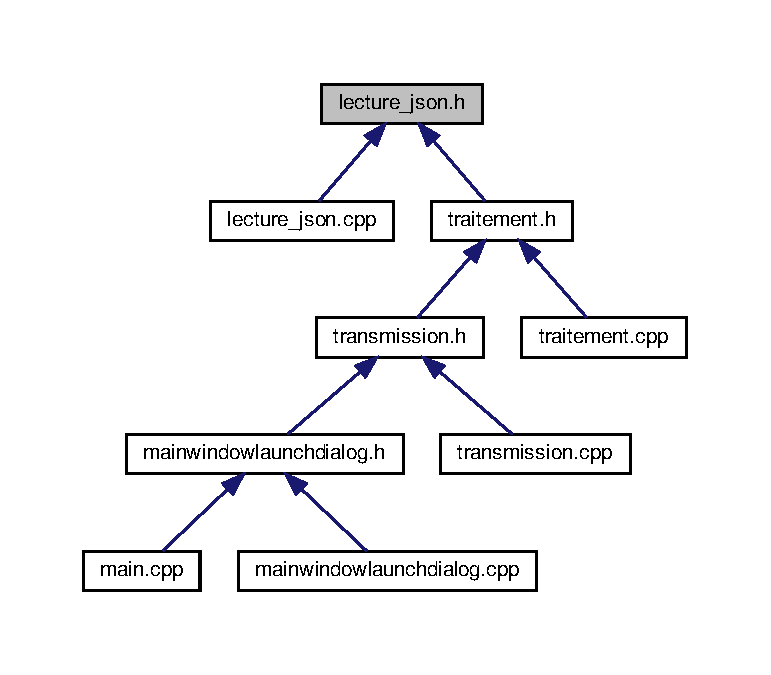
\includegraphics[width=350pt]{lecture__json_8h__dep__incl}
\end{center}
\end{figure}
\doxysubsection*{Classes}
\begin{DoxyCompactItemize}
\item 
class \mbox{\hyperlink{classlecture__json}{lecture\+\_\+json}}
\end{DoxyCompactItemize}


\doxysubsection{Detailed Description}
Classe gérant la lecture du fichier json. 

\begin{DoxyAuthor}{Author}
Pollet Lucas -\/ Fougerouse Arsène 
\end{DoxyAuthor}

\hypertarget{main_8cpp}{}\section{Référence du fichier main.\+cpp}
\label{main_8cpp}\index{main.\+cpp@{main.\+cpp}}


Classe principale qui permet de lancer la première fenetre.  


{\ttfamily \#include \char`\"{}mainwindow.\+h\char`\"{}}\newline
{\ttfamily \#include \char`\"{}mainwindowlaunchdialog.\+h\char`\"{}}\newline
{\ttfamily \#include \char`\"{}recette.\+h\char`\"{}}\newline
{\ttfamily \#include $<$Q\+Application$>$}\newline
{\ttfamily \#include $<$Q\+Object$>$}\newline
Graphe des dépendances par inclusion de main.\+cpp\+:\nopagebreak
\begin{figure}[H]
\begin{center}
\leavevmode
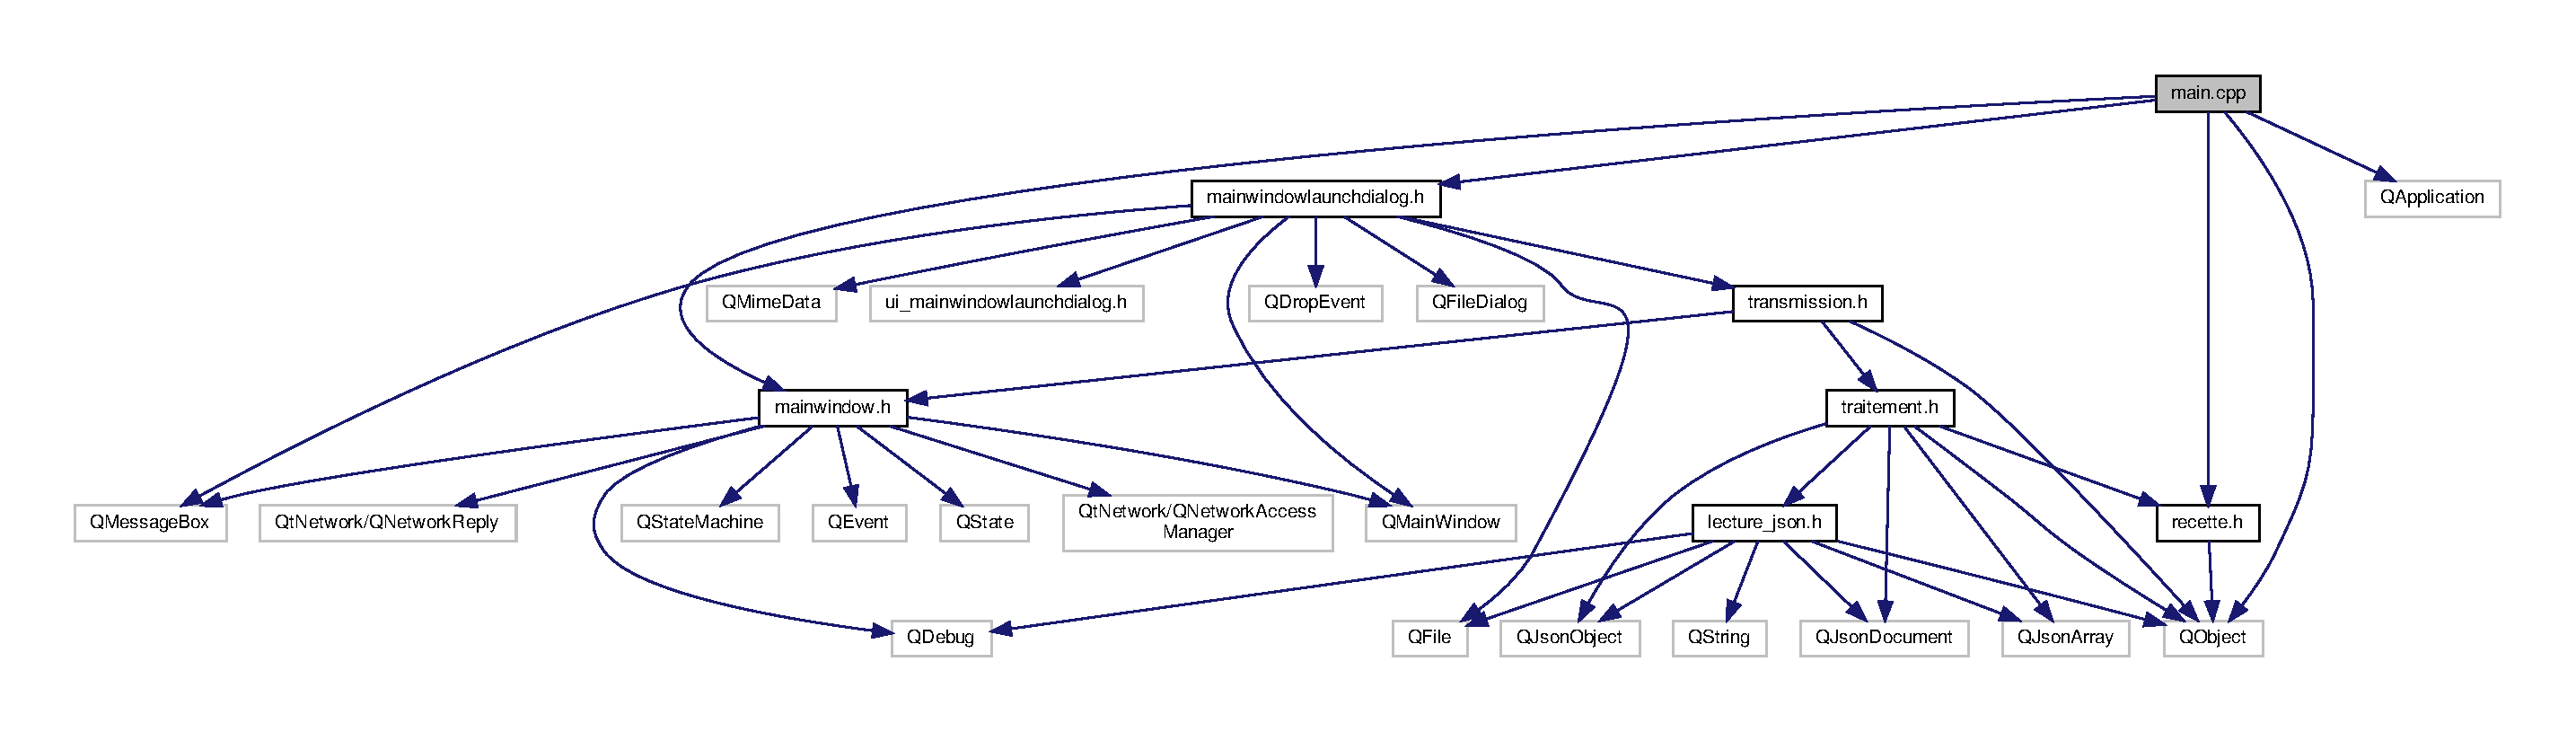
\includegraphics[width=350pt]{main_8cpp__incl}
\end{center}
\end{figure}
\subsection*{Fonctions}
\begin{DoxyCompactItemize}
\item 
int \hyperlink{main_8cpp_a0ddf1224851353fc92bfbff6f499fa97}{main} (int argc, char $\ast$argv\mbox{[}$\,$\mbox{]})
\end{DoxyCompactItemize}


\subsection{Description détaillée}
Classe principale qui permet de lancer la première fenetre. 

\begin{DoxyAuthor}{Auteur}
Pollet Lucas -\/ Fougerouse Arsène 
\end{DoxyAuthor}


\subsection{Documentation des fonctions}
\mbox{\Hypertarget{main_8cpp_a0ddf1224851353fc92bfbff6f499fa97}\label{main_8cpp_a0ddf1224851353fc92bfbff6f499fa97}} 
\index{main.\+cpp@{main.\+cpp}!main@{main}}
\index{main@{main}!main.\+cpp@{main.\+cpp}}
\subsubsection{\texorpdfstring{main()}{main()}}
{\footnotesize\ttfamily int main (\begin{DoxyParamCaption}\item[{int}]{argc,  }\item[{char $\ast$}]{argv\mbox{[}$\,$\mbox{]} }\end{DoxyParamCaption})}


\hypertarget{mainwindow_8cpp}{}\section{Référence du fichier mainwindow.\+cpp}
\label{mainwindow_8cpp}\index{mainwindow.\+cpp@{mainwindow.\+cpp}}


Classe de la fenêtre permettant l\textquotesingle{}affichage de la recette.  


{\ttfamily \#include \char`\"{}mainwindow.\+h\char`\"{}}\newline
{\ttfamily \#include \char`\"{}ui\+\_\+mainwindow.\+h\char`\"{}}\newline
Graphe des dépendances par inclusion de mainwindow.\+cpp\+:\nopagebreak
\begin{figure}[H]
\begin{center}
\leavevmode
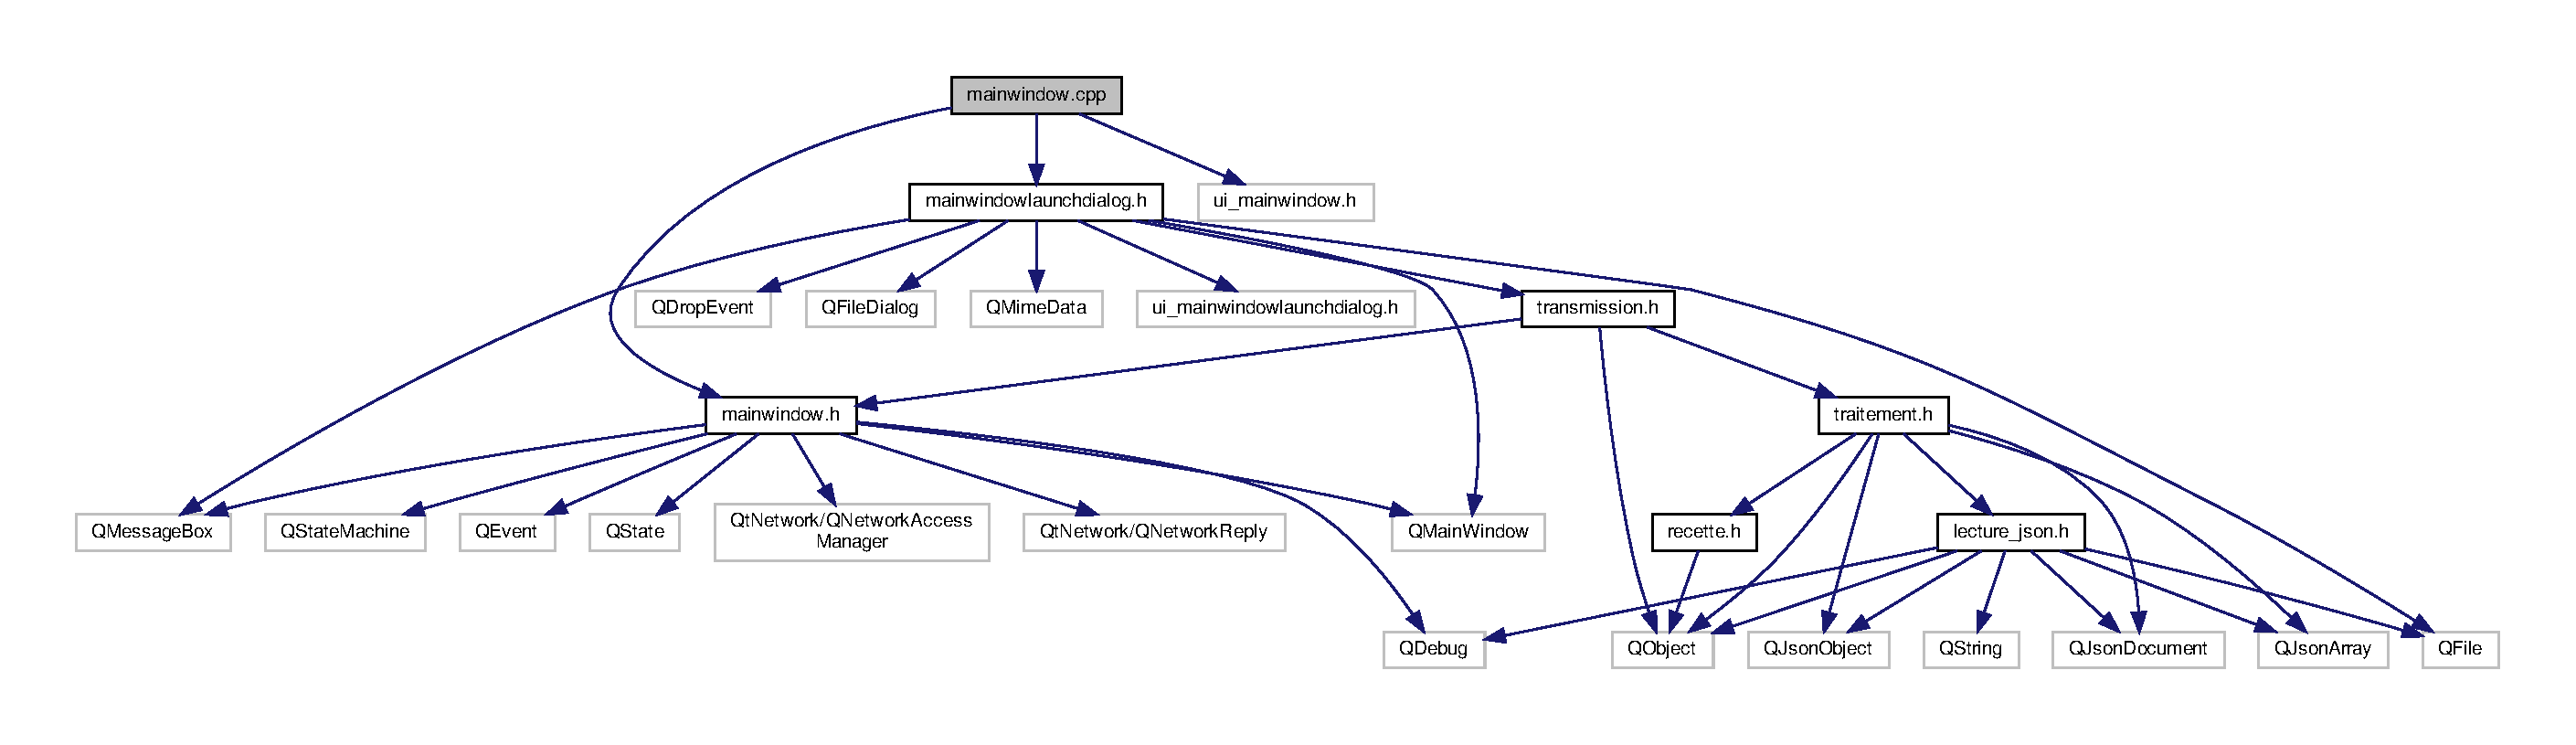
\includegraphics[width=350pt]{mainwindow_8cpp__incl}
\end{center}
\end{figure}


\subsection{Description détaillée}
Classe de la fenêtre permettant l\textquotesingle{}affichage de la recette. 

\begin{DoxyAuthor}{Auteur}
Pollet Lucas -\/ Fougerouse Arsène 
\end{DoxyAuthor}

\hypertarget{mainwindow_8h}{}\section{Référence du fichier mainwindow.\+h}
\label{mainwindow_8h}\index{mainwindow.\+h@{mainwindow.\+h}}


Classe qui affiche les informations nécessaires pour préparer la recette.  


{\ttfamily \#include $<$Q\+Main\+Window$>$}\newline
{\ttfamily \#include $<$Q\+State\+Machine$>$}\newline
{\ttfamily \#include $<$Q\+Debug$>$}\newline
{\ttfamily \#include $<$Q\+Event$>$}\newline
{\ttfamily \#include $<$Q\+Message\+Box$>$}\newline
{\ttfamily \#include $<$Q\+State$>$}\newline
{\ttfamily \#include $<$Qt\+Network/\+Q\+Network\+Access\+Manager$>$}\newline
{\ttfamily \#include $<$Qt\+Network/\+Q\+Network\+Reply$>$}\newline
Graphe des dépendances par inclusion de mainwindow.\+h\+:\nopagebreak
\begin{figure}[H]
\begin{center}
\leavevmode
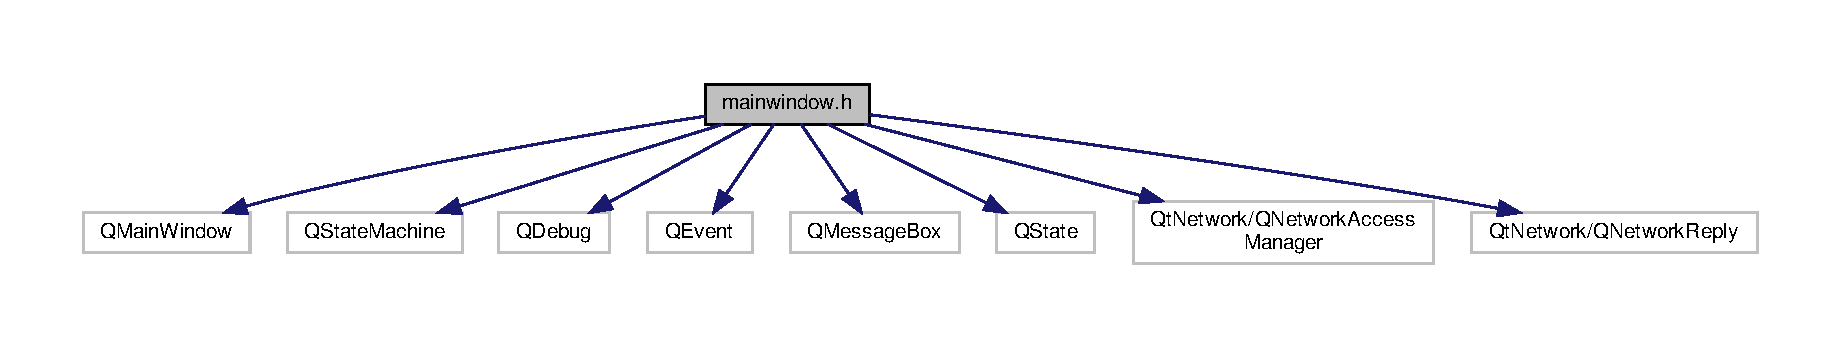
\includegraphics[width=350pt]{mainwindow_8h__incl}
\end{center}
\end{figure}
Ce graphe montre quels fichiers incluent directement ou indirectement ce fichier \+:\nopagebreak
\begin{figure}[H]
\begin{center}
\leavevmode
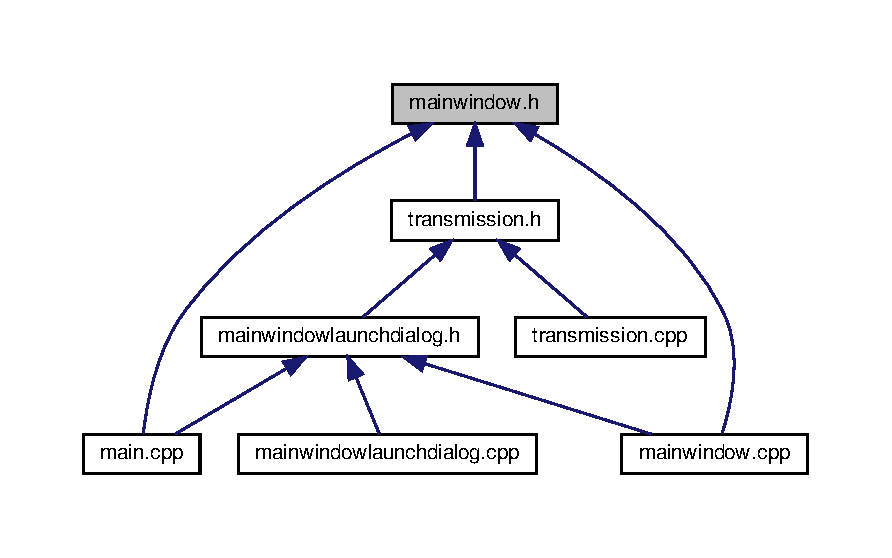
\includegraphics[width=350pt]{mainwindow_8h__dep__incl}
\end{center}
\end{figure}
\subsection*{Classes}
\begin{DoxyCompactItemize}
\item 
class \hyperlink{classMainWindow}{Main\+Window}
\end{DoxyCompactItemize}
\subsection*{Espaces de nommage}
\begin{DoxyCompactItemize}
\item 
 \hyperlink{namespaceUi}{Ui}
\end{DoxyCompactItemize}


\subsection{Description détaillée}
Classe qui affiche les informations nécessaires pour préparer la recette. 

\begin{DoxyAuthor}{Auteur}
Pollet Lucas -\/ Fougerouse Arsène 
\end{DoxyAuthor}
\begin{DoxyDate}{Date}
mai 2020 
\end{DoxyDate}

\hypertarget{mainwindowlaunchdialog_8cpp}{}\doxysection{mainwindowlaunchdialog.\+cpp File Reference}
\label{mainwindowlaunchdialog_8cpp}\index{mainwindowlaunchdialog.cpp@{mainwindowlaunchdialog.cpp}}


Classe de la fenêtre permettant le choix du fichier json de recette.  


{\ttfamily \#include \char`\"{}mainwindow.\+h\char`\"{}}\newline
{\ttfamily \#include \char`\"{}mainwindowlaunchdialog.\+h\char`\"{}}\newline
{\ttfamily \#include \char`\"{}ui\+\_\+mainwindowlaunchdialog.\+h\char`\"{}}\newline
{\ttfamily \#include $<$Q\+File$>$}\newline
{\ttfamily \#include $<$Q\+File\+Dialog$>$}\newline
{\ttfamily \#include $<$Q\+Message\+Box$>$}\newline
{\ttfamily \#include $<$Q\+Mime\+Data$>$}\newline
{\ttfamily \#include $<$lecture\+\_\+json.\+h$>$}\newline
Include dependency graph for mainwindowlaunchdialog.\+cpp\+:\nopagebreak
\begin{figure}[H]
\begin{center}
\leavevmode
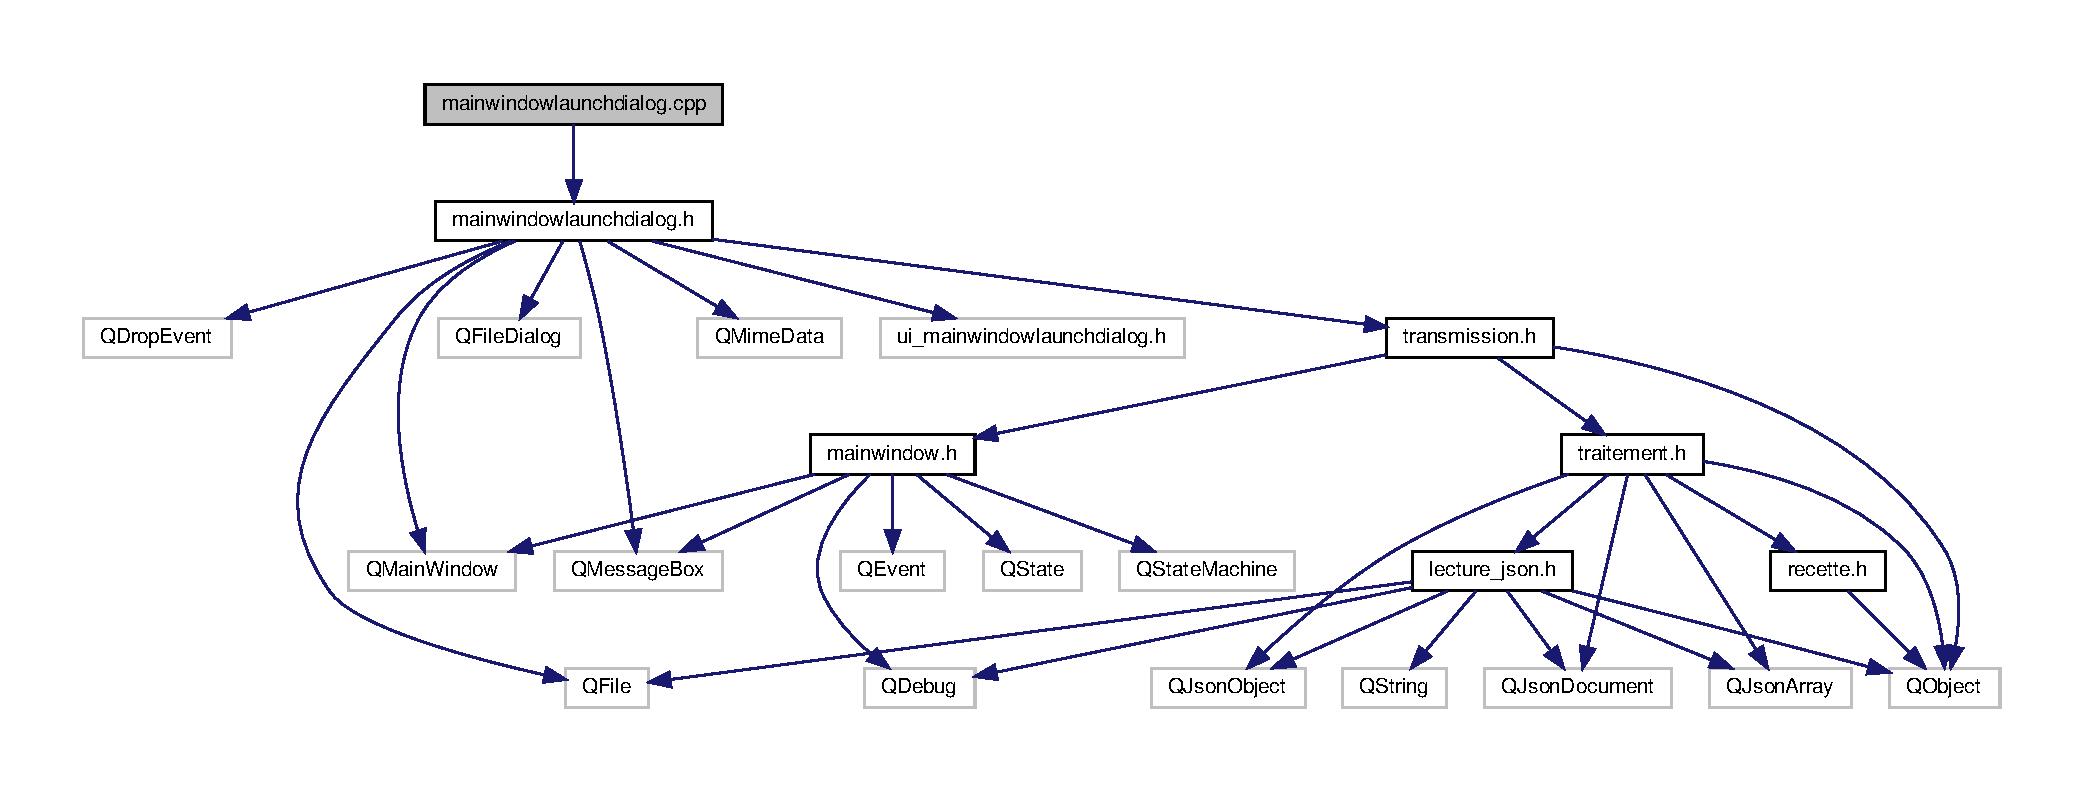
\includegraphics[width=350pt]{mainwindowlaunchdialog_8cpp__incl}
\end{center}
\end{figure}


\doxysubsection{Detailed Description}
Classe de la fenêtre permettant le choix du fichier json de recette. 

\begin{DoxyAuthor}{Author}
Pollet Lucas -\/ Fougerouse Arsène 
\end{DoxyAuthor}

\hypertarget{mainwindowlaunchdialog_8h}{}\section{Référence du fichier mainwindowlaunchdialog.\+h}
\label{mainwindowlaunchdialog_8h}\index{mainwindowlaunchdialog.\+h@{mainwindowlaunchdialog.\+h}}


Classe de la fenêtre permettant le choix du fichier json de recette.  


{\ttfamily \#include $<$Q\+Drop\+Event$>$}\newline
{\ttfamily \#include $<$Q\+Main\+Window$>$}\newline
{\ttfamily \#include $<$Q\+File$>$}\newline
{\ttfamily \#include $<$Q\+File\+Dialog$>$}\newline
{\ttfamily \#include $<$Q\+Message\+Box$>$}\newline
{\ttfamily \#include $<$Q\+Mime\+Data$>$}\newline
{\ttfamily \#include \char`\"{}ui\+\_\+mainwindowlaunchdialog.\+h\char`\"{}}\newline
{\ttfamily \#include \char`\"{}transmission.\+h\char`\"{}}\newline
Graphe des dépendances par inclusion de mainwindowlaunchdialog.\+h\+:\nopagebreak
\begin{figure}[H]
\begin{center}
\leavevmode
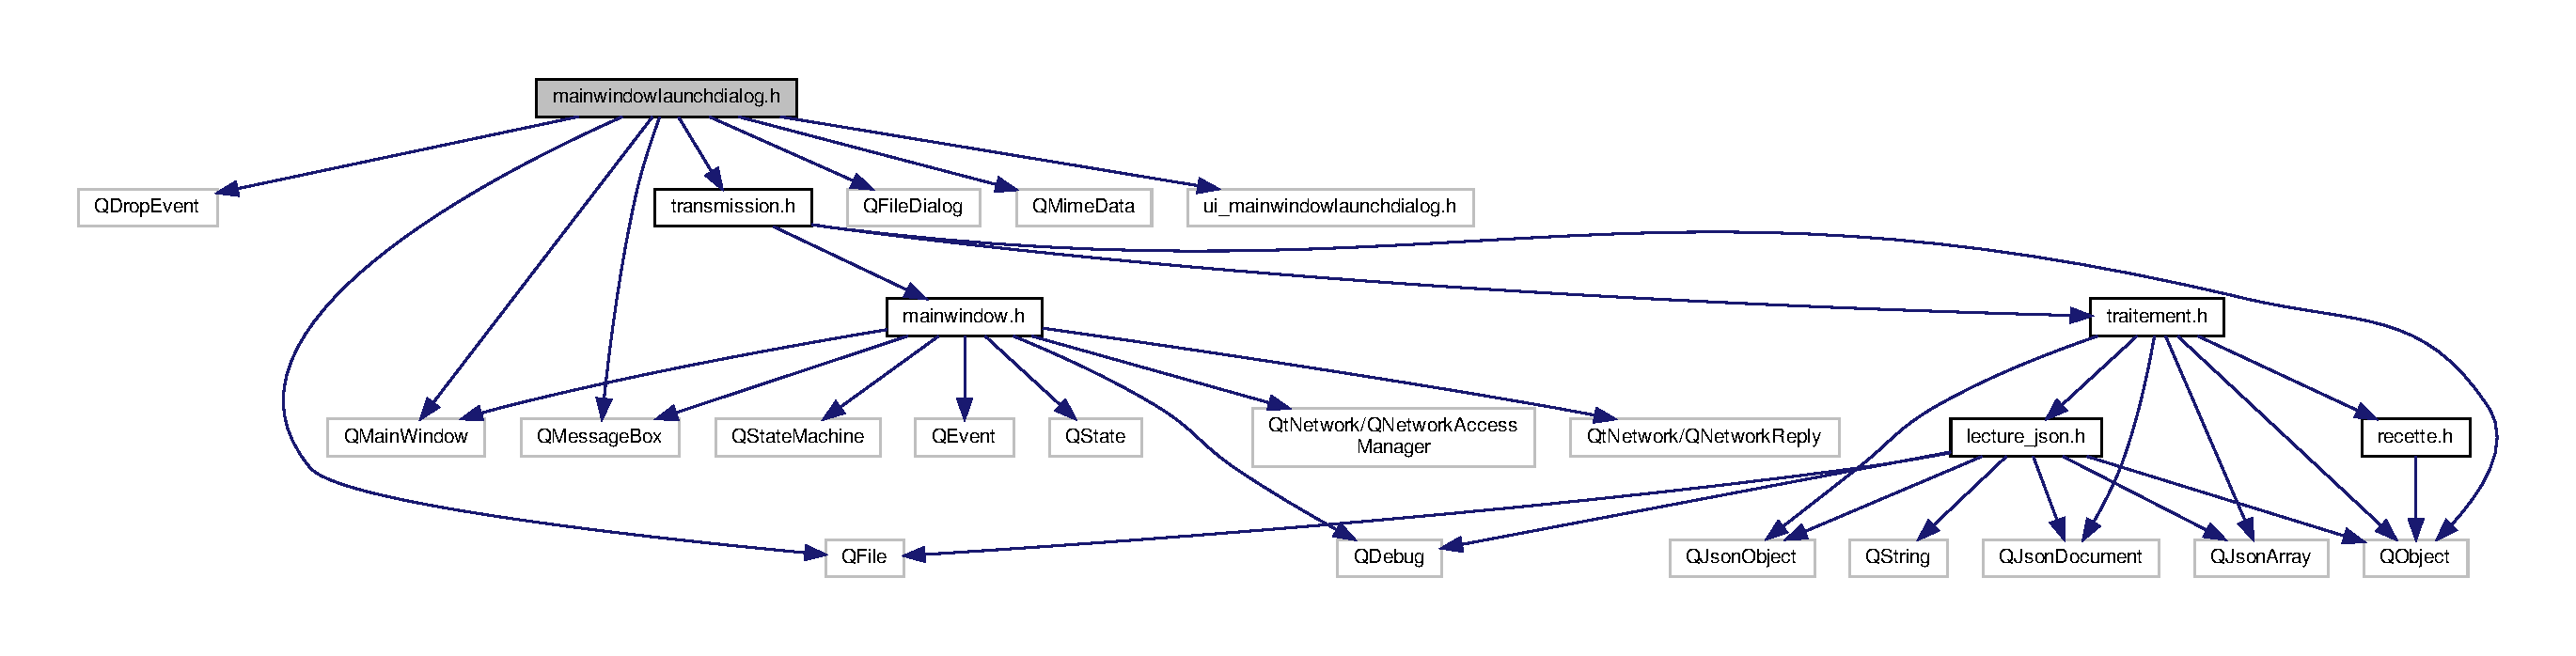
\includegraphics[width=350pt]{mainwindowlaunchdialog_8h__incl}
\end{center}
\end{figure}
Ce graphe montre quels fichiers incluent directement ou indirectement ce fichier \+:\nopagebreak
\begin{figure}[H]
\begin{center}
\leavevmode
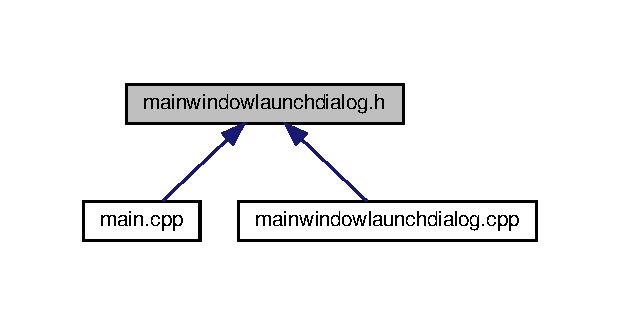
\includegraphics[width=298pt]{mainwindowlaunchdialog_8h__dep__incl}
\end{center}
\end{figure}
\subsection*{Classes}
\begin{DoxyCompactItemize}
\item 
class \hyperlink{classMainWindowLaunchDialog}{Main\+Window\+Launch\+Dialog}
\end{DoxyCompactItemize}
\subsection*{Espaces de nommage}
\begin{DoxyCompactItemize}
\item 
 \hyperlink{namespaceUi}{Ui}
\end{DoxyCompactItemize}


\subsection{Description détaillée}
Classe de la fenêtre permettant le choix du fichier json de recette. 

\begin{DoxyAuthor}{Auteur}
Pollet Lucas -\/ Fougerouse Arsène 
\end{DoxyAuthor}

\hypertarget{README_8md}{}\doxysection{R\+E\+A\+D\+M\+E.\+md File Reference}
\label{README_8md}\index{README.md@{README.md}}

\hypertarget{recette_8cpp}{}\section{Référence du fichier recette.\+cpp}
\label{recette_8cpp}\index{recette.\+cpp@{recette.\+cpp}}


Classe permettant la gestion et le stockage de la recette.  


{\ttfamily \#include \char`\"{}recette.\+h\char`\"{}}\newline
Graphe des dépendances par inclusion de recette.\+cpp\+:\nopagebreak
\begin{figure}[H]
\begin{center}
\leavevmode
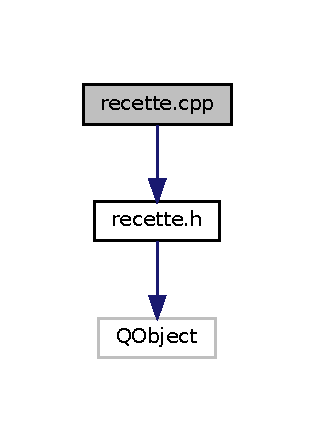
\includegraphics[width=145pt]{recette_8cpp__incl}
\end{center}
\end{figure}


\subsection{Description détaillée}
Classe permettant la gestion et le stockage de la recette. 

\begin{DoxyAuthor}{Auteur}
Pollet Lucas -\/ Fougerouse Arsène 
\end{DoxyAuthor}

\hypertarget{recette_8h}{}\section{Référence du fichier recette.\+h}
\label{recette_8h}\index{recette.\+h@{recette.\+h}}


Classe qui stocke sous forme d\textquotesingle{}attribut les informations d\textquotesingle{}une recette.  


{\ttfamily \#include $<$Q\+Object$>$}\newline
Graphe des dépendances par inclusion de recette.\+h\+:\nopagebreak
\begin{figure}[H]
\begin{center}
\leavevmode
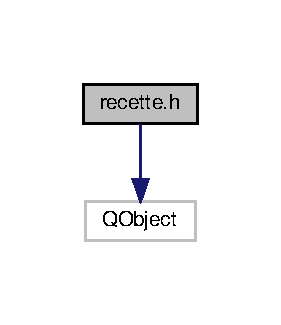
\includegraphics[width=135pt]{recette_8h__incl}
\end{center}
\end{figure}
Ce graphe montre quels fichiers incluent directement ou indirectement ce fichier \+:\nopagebreak
\begin{figure}[H]
\begin{center}
\leavevmode
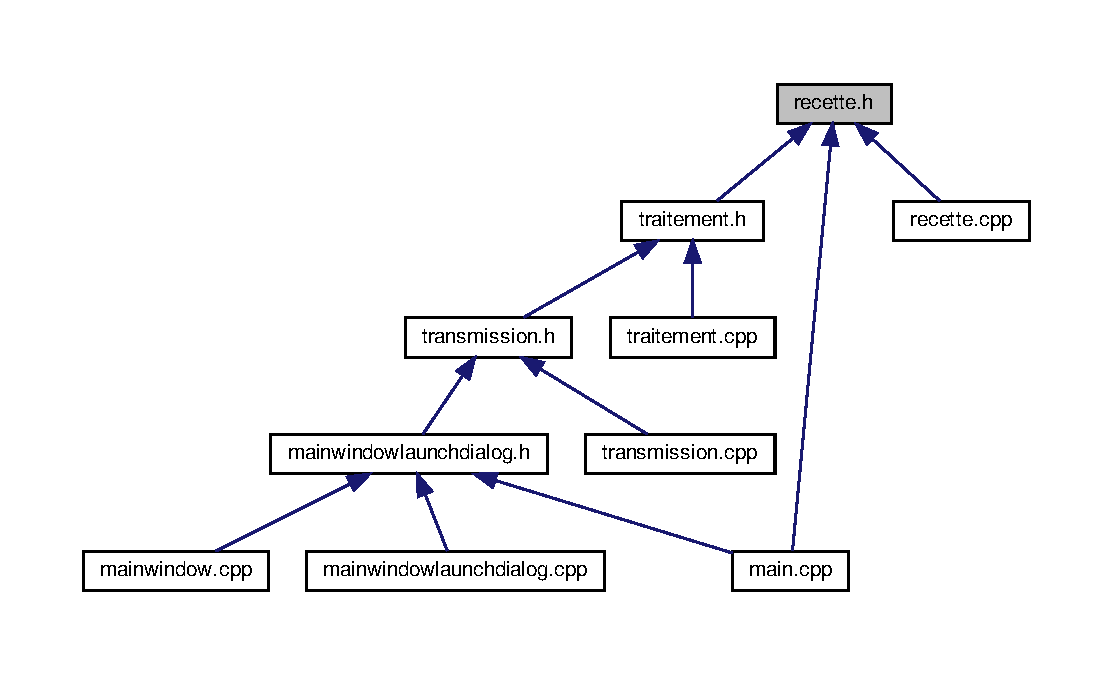
\includegraphics[width=350pt]{recette_8h__dep__incl}
\end{center}
\end{figure}
\subsection*{Classes}
\begin{DoxyCompactItemize}
\item 
class \hyperlink{classRecette}{Recette}
\end{DoxyCompactItemize}


\subsection{Description détaillée}
Classe qui stocke sous forme d\textquotesingle{}attribut les informations d\textquotesingle{}une recette. 

\begin{DoxyAuthor}{Auteur}
Pollet Lucas -\/ Fougerouse Arsène 
\end{DoxyAuthor}
\begin{DoxyDate}{Date}
mai 2020 
\end{DoxyDate}

\hypertarget{traitement_8cpp}{}\section{traitement.\+cpp File Reference}
\label{traitement_8cpp}\index{traitement.\+cpp@{traitement.\+cpp}}


Classe permettant le traitement json.  


{\ttfamily \#include \char`\"{}traitement.\+h\char`\"{}}\newline
Include dependency graph for traitement.\+cpp\+:\nopagebreak
\begin{figure}[H]
\begin{center}
\leavevmode
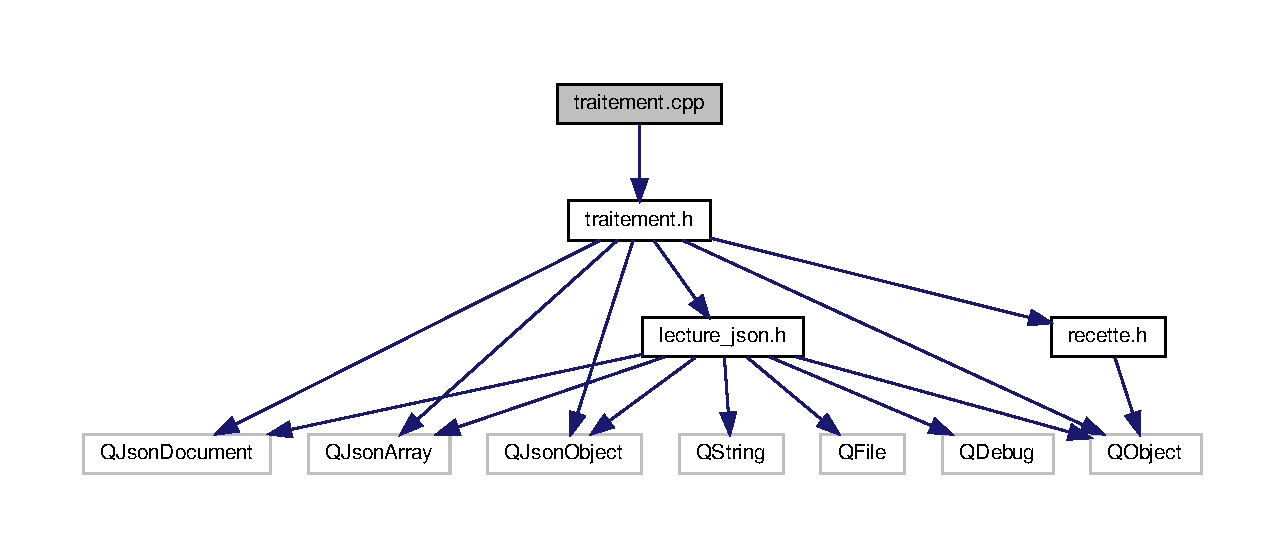
\includegraphics[width=350pt]{traitement_8cpp__incl}
\end{center}
\end{figure}


\subsection{Detailed Description}
Classe permettant le traitement json. 

\begin{DoxyAuthor}{Author}
Pollet Lucas -\/ Fougerouse Arsène 
\end{DoxyAuthor}

\hypertarget{traitement_8h}{}\doxysection{traitement.\+h File Reference}
\label{traitement_8h}\index{traitement.h@{traitement.h}}


Classe permettant le traitement json.  


{\ttfamily \#include $<$Q\+Json\+Document$>$}\newline
{\ttfamily \#include $<$Q\+Json\+Array$>$}\newline
{\ttfamily \#include $<$Q\+Json\+Object$>$}\newline
{\ttfamily \#include \char`\"{}recette.\+h\char`\"{}}\newline
{\ttfamily \#include \char`\"{}mainwindow.\+h\char`\"{}}\newline
Include dependency graph for traitement.\+h\+:\nopagebreak
\begin{figure}[H]
\begin{center}
\leavevmode
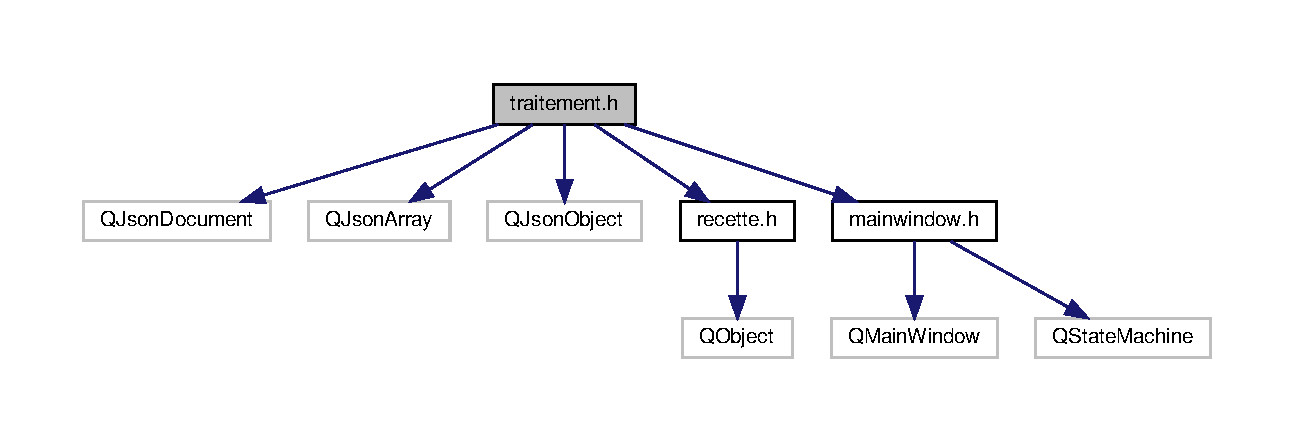
\includegraphics[width=350pt]{traitement_8h__incl}
\end{center}
\end{figure}
This graph shows which files directly or indirectly include this file\+:\nopagebreak
\begin{figure}[H]
\begin{center}
\leavevmode
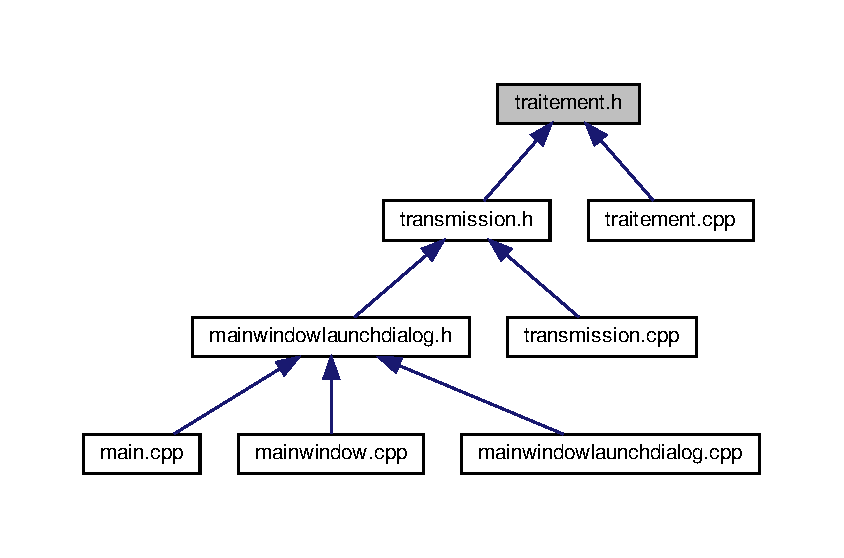
\includegraphics[width=284pt]{traitement_8h__dep__incl}
\end{center}
\end{figure}
\doxysubsection*{Classes}
\begin{DoxyCompactItemize}
\item 
class \mbox{\hyperlink{classtraitement}{traitement}}
\end{DoxyCompactItemize}


\doxysubsection{Detailed Description}
Classe permettant le traitement json. 

\begin{DoxyAuthor}{Author}
Pollet Lucas -\/ Fougerouse Arsène 
\end{DoxyAuthor}

\hypertarget{transmission_8cpp}{}\section{Référence du fichier transmission.\+cpp}
\label{transmission_8cpp}\index{transmission.\+cpp@{transmission.\+cpp}}
{\ttfamily \#include \char`\"{}transmission.\+h\char`\"{}}\newline
Graphe des dépendances par inclusion de transmission.\+cpp\+:\nopagebreak
\begin{figure}[H]
\begin{center}
\leavevmode
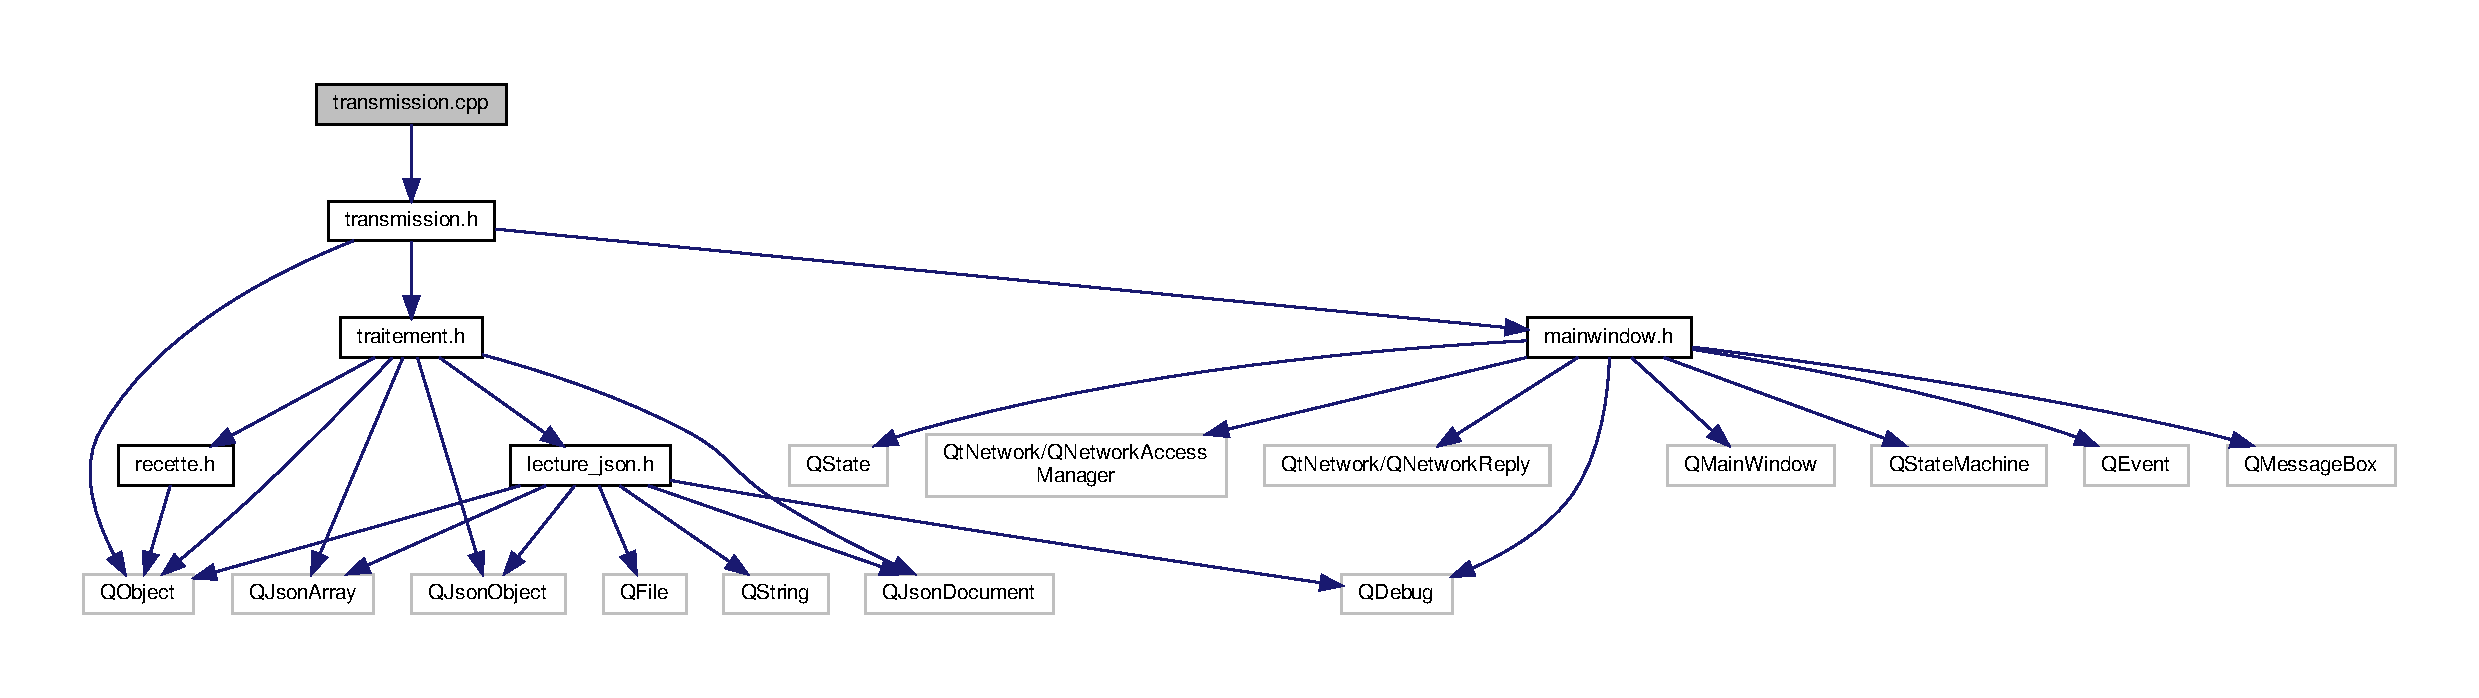
\includegraphics[width=350pt]{transmission_8cpp__incl}
\end{center}
\end{figure}

\hypertarget{transmission_8h}{}\section{Référence du fichier transmission.\+h}
\label{transmission_8h}\index{transmission.\+h@{transmission.\+h}}


Classe permettant le transmission des données.  


{\ttfamily \#include $<$Q\+Object$>$}\newline
{\ttfamily \#include \char`\"{}mainwindow.\+h\char`\"{}}\newline
{\ttfamily \#include \char`\"{}traitement.\+h\char`\"{}}\newline
Graphe des dépendances par inclusion de transmission.\+h\+:\nopagebreak
\begin{figure}[H]
\begin{center}
\leavevmode
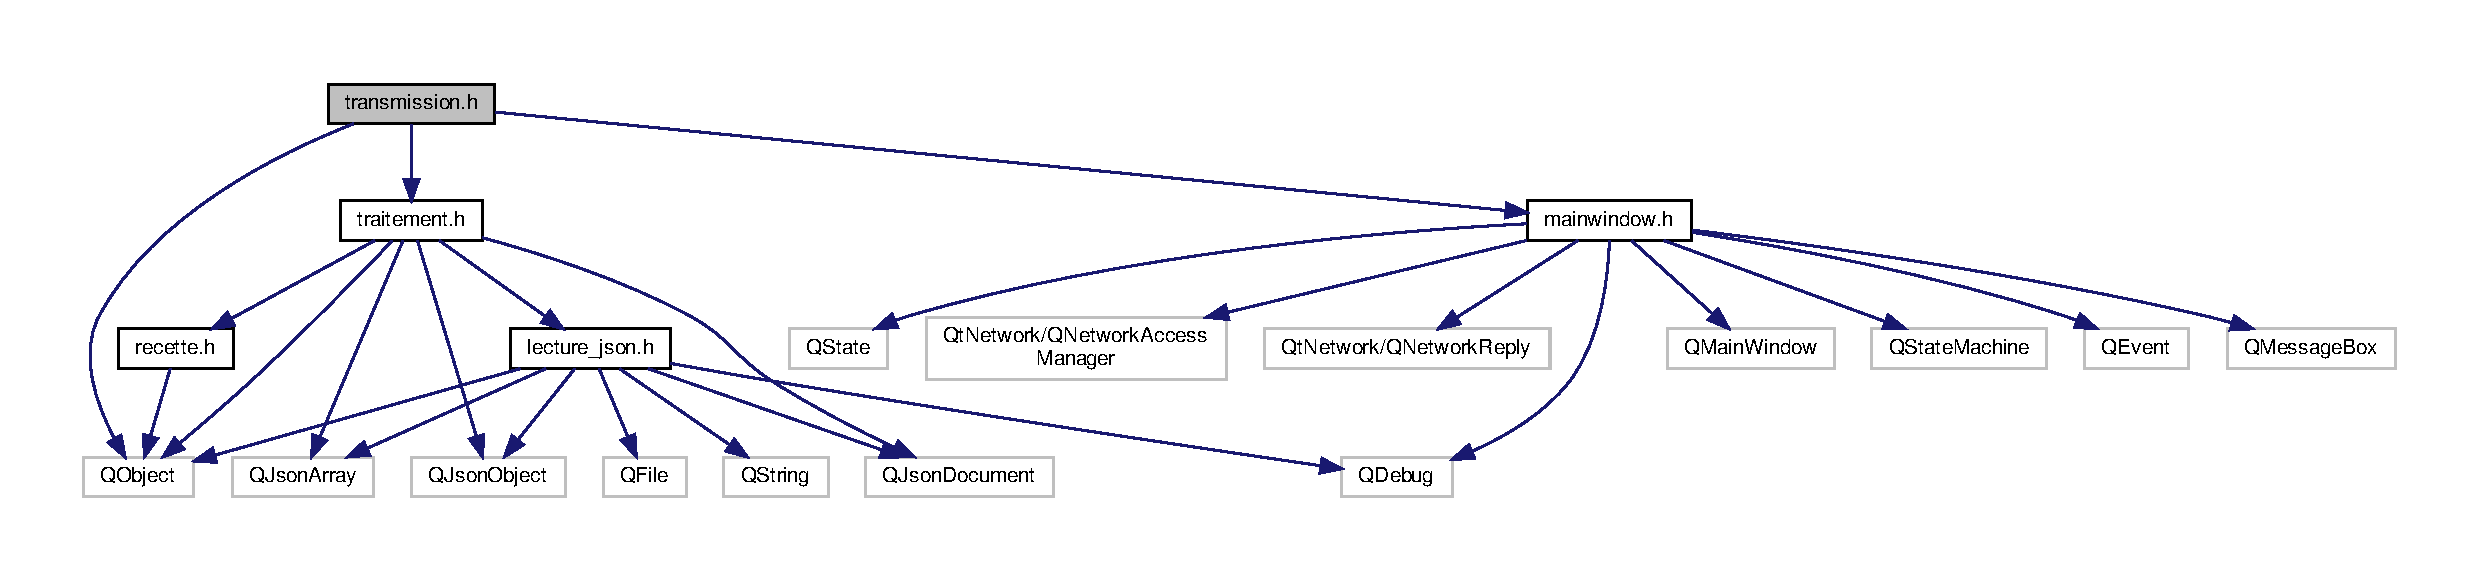
\includegraphics[width=350pt]{transmission_8h__incl}
\end{center}
\end{figure}
Ce graphe montre quels fichiers incluent directement ou indirectement ce fichier \+:\nopagebreak
\begin{figure}[H]
\begin{center}
\leavevmode
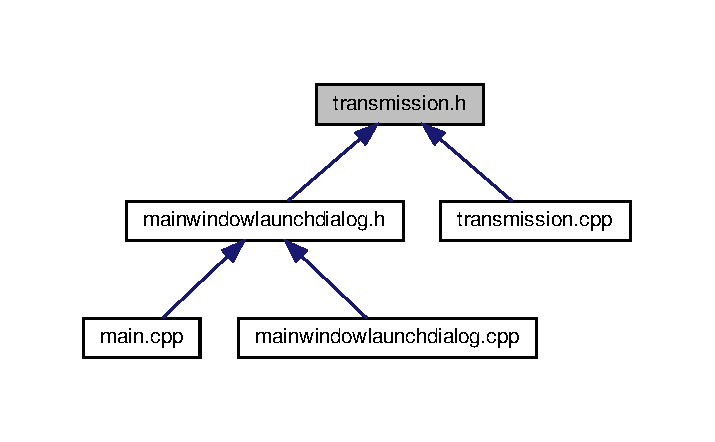
\includegraphics[width=350pt]{transmission_8h__dep__incl}
\end{center}
\end{figure}
\subsection*{Classes}
\begin{DoxyCompactItemize}
\item 
class \hyperlink{classTransmission}{Transmission}
\end{DoxyCompactItemize}


\subsection{Description détaillée}
Classe permettant le transmission des données. 

\begin{DoxyAuthor}{Auteur}
Pollet Lucas -\/ Fougerouse Arsène 
\end{DoxyAuthor}

\hypertarget{ui__mainwindow_8h}{}\section{Référence du fichier ui\+\_\+mainwindow.\+h}
\label{ui__mainwindow_8h}\index{ui\+\_\+mainwindow.\+h@{ui\+\_\+mainwindow.\+h}}
{\ttfamily \#include $<$Qt\+Core/\+Q\+Variant$>$}\newline
{\ttfamily \#include $<$Qt\+Widgets/\+Q\+Application$>$}\newline
{\ttfamily \#include $<$Qt\+Widgets/\+Q\+H\+Box\+Layout$>$}\newline
{\ttfamily \#include $<$Qt\+Widgets/\+Q\+Label$>$}\newline
{\ttfamily \#include $<$Qt\+Widgets/\+Q\+Main\+Window$>$}\newline
{\ttfamily \#include $<$Qt\+Widgets/\+Q\+Menu\+Bar$>$}\newline
{\ttfamily \#include $<$Qt\+Widgets/\+Q\+Push\+Button$>$}\newline
{\ttfamily \#include $<$Qt\+Widgets/\+Q\+Status\+Bar$>$}\newline
{\ttfamily \#include $<$Qt\+Widgets/\+Q\+Tab\+Widget$>$}\newline
{\ttfamily \#include $<$Qt\+Widgets/\+Q\+V\+Box\+Layout$>$}\newline
{\ttfamily \#include $<$Qt\+Widgets/\+Q\+Widget$>$}\newline
Graphe des dépendances par inclusion de ui\+\_\+mainwindow.\+h\+:\nopagebreak
\begin{figure}[H]
\begin{center}
\leavevmode
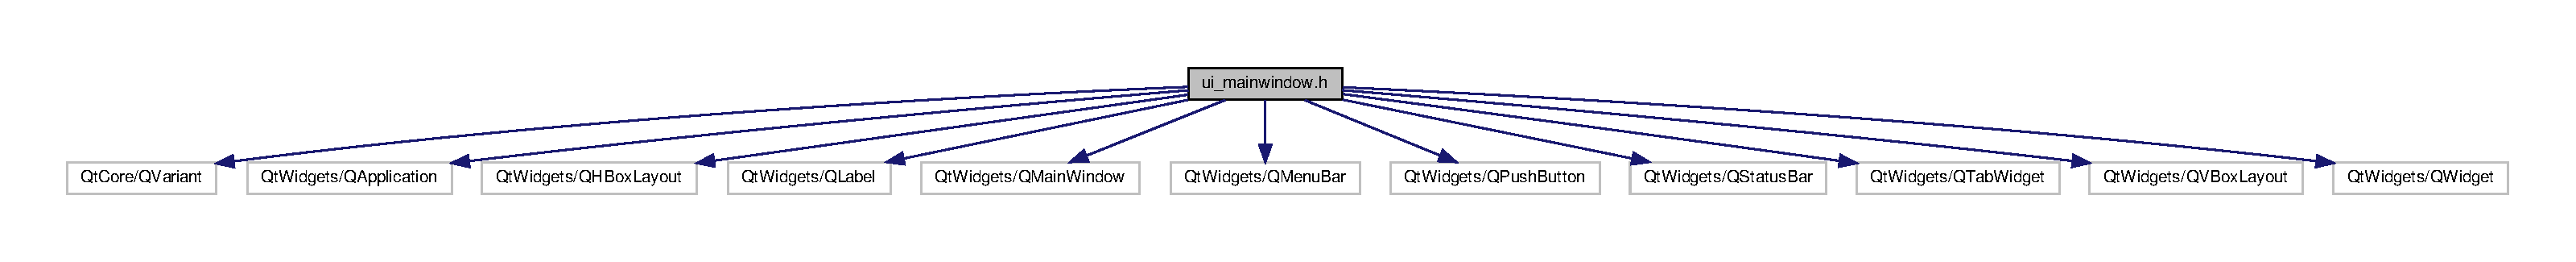
\includegraphics[width=350pt]{ui__mainwindow_8h__incl}
\end{center}
\end{figure}
Ce graphe montre quels fichiers incluent directement ou indirectement ce fichier \+:\nopagebreak
\begin{figure}[H]
\begin{center}
\leavevmode
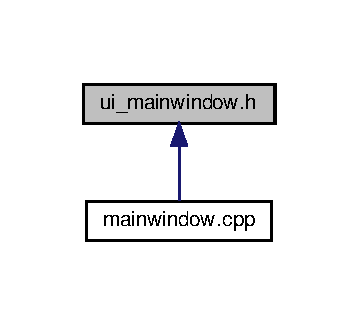
\includegraphics[width=172pt]{ui__mainwindow_8h__dep__incl}
\end{center}
\end{figure}
\subsection*{Classes}
\begin{DoxyCompactItemize}
\item 
class \hyperlink{classUi__MainWindow}{Ui\+\_\+\+Main\+Window}
\item 
class \hyperlink{classUi_1_1MainWindow}{Ui\+::\+Main\+Window}
\end{DoxyCompactItemize}
\subsection*{Espaces de nommage}
\begin{DoxyCompactItemize}
\item 
 \hyperlink{namespaceUi}{Ui}
\end{DoxyCompactItemize}

\hypertarget{ui__mainwindowlaunchdialog_8h}{}\section{Référence du fichier ui\+\_\+mainwindowlaunchdialog.\+h}
\label{ui__mainwindowlaunchdialog_8h}\index{ui\+\_\+mainwindowlaunchdialog.\+h@{ui\+\_\+mainwindowlaunchdialog.\+h}}
{\ttfamily \#include $<$Qt\+Core/\+Q\+Variant$>$}\newline
{\ttfamily \#include $<$Qt\+Widgets/\+Q\+Action$>$}\newline
{\ttfamily \#include $<$Qt\+Widgets/\+Q\+Application$>$}\newline
{\ttfamily \#include $<$Qt\+Widgets/\+Q\+Label$>$}\newline
{\ttfamily \#include $<$Qt\+Widgets/\+Q\+Main\+Window$>$}\newline
{\ttfamily \#include $<$Qt\+Widgets/\+Q\+Menu$>$}\newline
{\ttfamily \#include $<$Qt\+Widgets/\+Q\+Menu\+Bar$>$}\newline
{\ttfamily \#include $<$Qt\+Widgets/\+Q\+Push\+Button$>$}\newline
{\ttfamily \#include $<$Qt\+Widgets/\+Q\+Status\+Bar$>$}\newline
{\ttfamily \#include $<$Qt\+Widgets/\+Q\+V\+Box\+Layout$>$}\newline
{\ttfamily \#include $<$Qt\+Widgets/\+Q\+Widget$>$}\newline
Graphe des dépendances par inclusion de ui\+\_\+mainwindowlaunchdialog.\+h\+:\nopagebreak
\begin{figure}[H]
\begin{center}
\leavevmode
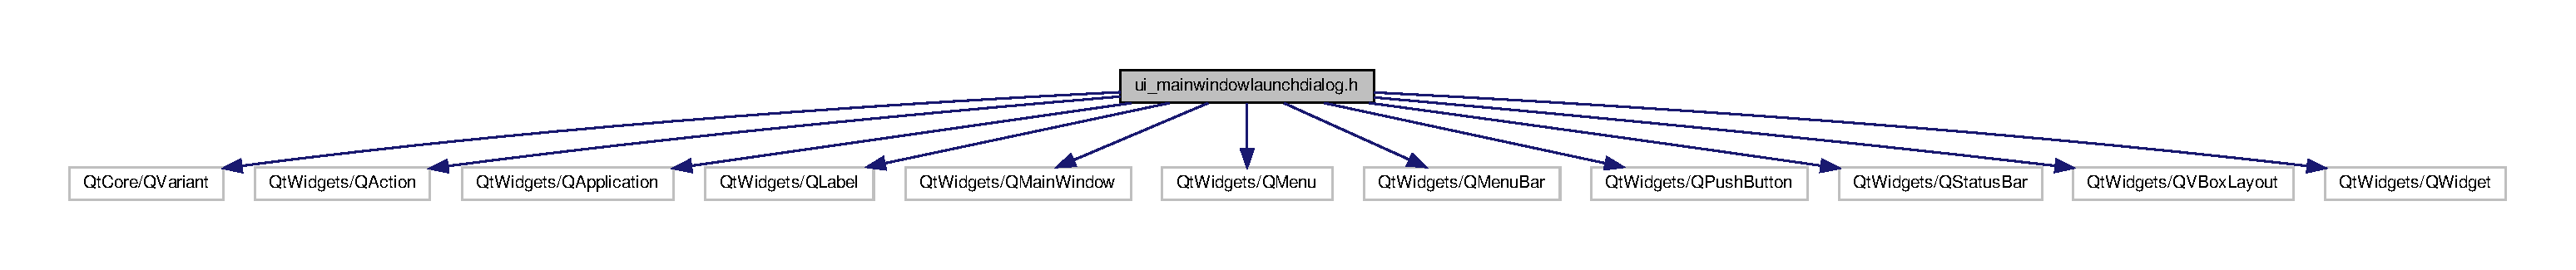
\includegraphics[width=350pt]{ui__mainwindowlaunchdialog_8h__incl}
\end{center}
\end{figure}
Ce graphe montre quels fichiers incluent directement ou indirectement ce fichier \+:\nopagebreak
\begin{figure}[H]
\begin{center}
\leavevmode
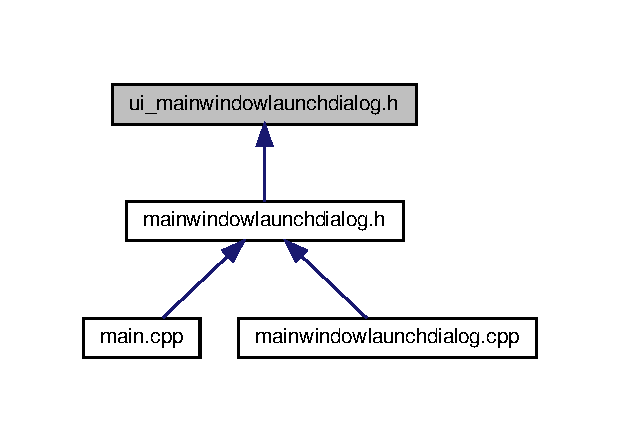
\includegraphics[width=298pt]{ui__mainwindowlaunchdialog_8h__dep__incl}
\end{center}
\end{figure}
\subsection*{Classes}
\begin{DoxyCompactItemize}
\item 
class \hyperlink{classUi__MainWindowLaunchDialog}{Ui\+\_\+\+Main\+Window\+Launch\+Dialog}
\item 
class \hyperlink{classUi_1_1MainWindowLaunchDialog}{Ui\+::\+Main\+Window\+Launch\+Dialog}
\end{DoxyCompactItemize}
\subsection*{Espaces de nommage}
\begin{DoxyCompactItemize}
\item 
 \hyperlink{namespaceUi}{Ui}
\end{DoxyCompactItemize}

%--- End generated contents ---

% Index
\backmatter
\newpage
\phantomsection
\clearemptydoublepage
\addcontentsline{toc}{chapter}{Index}
\printindex

\end{document}
